% !TEX TS-program = xelatex
% !TEX ecoding = UTF-8

\documentclass[10pt]{beamer}

\usepackage{xeCJK}
\setCJKmainfont{Noto Sans CJK SC}
\xeCJKsetup{PunctStyle=kaiming,CJKspace=true,CheckSingle=true} 

\usepackage{subfigure}
\usepackage{amssymb, amsmath, amsfonts,verbatim}
\usepackage{tikz}
\graphicspath{ {./} }
\usetikzlibrary{matrix,arrows,fit,backgrounds,mindmap,plotmarks,decorations.pathreplacing}
%\usepackage{tkz-euclide}
\usepackage{pgfplots}
\pgfplotsset{compat=1.12}
\pgfdeclarelayer{background}
\pgfsetlayers{background,main}

\usepackage{esvect}
\usepackage[citestyle=authortitle,backend=bibtex]{biblatex}
\addbibresource{references.bib}
\tikzset{decoration={name=none},}

\newlength\figureheight
\newlength\figurewidth

\newcommand{\tikzdir}[1]{#1.tikz}
\newcommand{\inputtikz}[1]{\input{\tikzdir{#1}}}

\newcommand{\tI}{\tilde {\mathcal I}}
\newcommand{\tA}{\tilde A}
\newcommand{\ty}{\tilde y}
\newcommand{\tx}{\tilde x}
\newcommand{\tw}{\tilde w}
\newcommand{\tv}{\tilde v}
\newcommand{\tC}{\tilde C}
\newcommand{\tP}{\tilde P}
\newcommand{\Ic}{{\mathcal I^c}}
\newcommand{\J}{{\mathcal J}}
\newcommand{\K}{{\mathcal K}}

\DeclareMathOperator{\Smin}{Smin}
\DeclareMathOperator{\Smid}{Smid}
\DeclareMathOperator{\Smax}{Smax}
\DeclareMathOperator{\MSE}{MSE}
\DeclareMathOperator{\rank}{rank}
\DeclareMathOperator{\Med}{Med}
\DeclareMathOperator{\Max}{Max}
\DeclareMathOperator{\Min}{Min}
\DeclareMathOperator{\tr}{tr}
\DeclareMathOperator{\Cov}{Cov}
\DeclareMathOperator{\logdet}{log\;det}
\DeclareMathOperator{\argmin}{arg\;min}
\DeclareMathOperator{\argmax}{arg\;max}
\let\Tiny\tiny

\title[Secure CPS]{信息物理系统中的安全控制算法设计}
\author[Yilin Mo]{Yilin Mo}
\institute[Tsinghua]{Department of Automation, Tsinghua University}
\date[June 21, 2021]{June 21, 2021}

\usetheme[subsectionpage=none,block=fill]{metropolis}
\definecolor{thupurple}{RGB}{102,8,116}
\definecolor{caltechcolor}{RGB}{102,8,116}
\setbeamercolor{title separator}{fg=black!50}
\setbeamercolor{frametitle}{bg=thupurple!70!black}


\begin{document}

\maketitle 

\section{Introduction}

\begin{frame}{Cyber-Physical System}
  \begin{itemize}
    \item Cyber-Physical Systems (CPSs) refer to the embedding of computation, communication and control into physical spaces.
      \begin{center}
	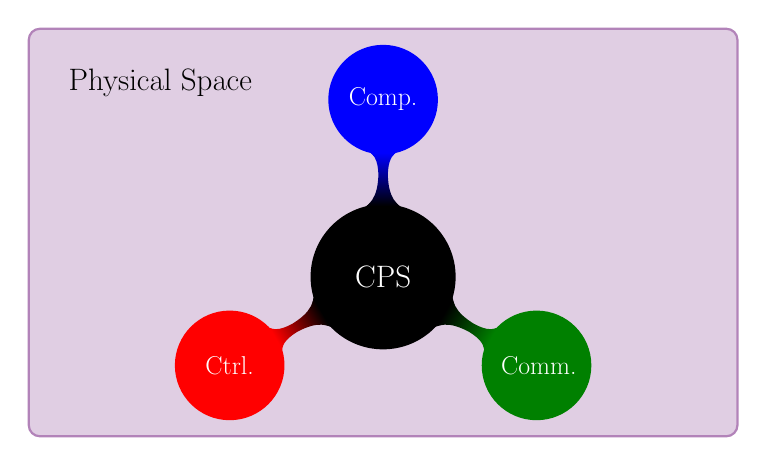
\begin{tikzpicture}[scale=0.45,transform shape,level distance=0cm,
	  level 1 concept/.append style={sibling angle=120,minimum size = 3cm},
	  ]
	  \path [draw=thupurple!50,fill=thupurple!20,thick,rounded corners] (-10,-4.5) rectangle (10,7);
	  \node at (-9,6) [anchor=north west] {\Huge Physical Space};
	  \path[mindmap,concept color=black,text=white]
	    node[concept] {\Huge CPS}
	    [clockwise from=330]
	    child[concept color=green!50!black] { node[concept](communication) {\huge Comm.} }
	    child[concept color=red] { node[concept](control) {\huge Ctrl.} }
	    child[concept color=blue] { node[concept](computation) {\huge Comp.} };
	\end{tikzpicture}
      \end{center}
    \item Applications: aerospace, chemical processes, civil infrastructure, energy, manufacturing and transportation. 
  \end{itemize}
\end{frame}

\begin{frame}{Security Threats for the CPS}
  \begin{itemize}
    \item The next generation CPS: Smart Grids, Smart Buildings, Smart Home, Internet of Things, will make extensive use of widespread sensing and networking.
    \item As the CPSs become ``smarter'', they are also more vulnerable to malicious attacks.
  \end{itemize}
  \begin{figure}[ht]
    \centering
    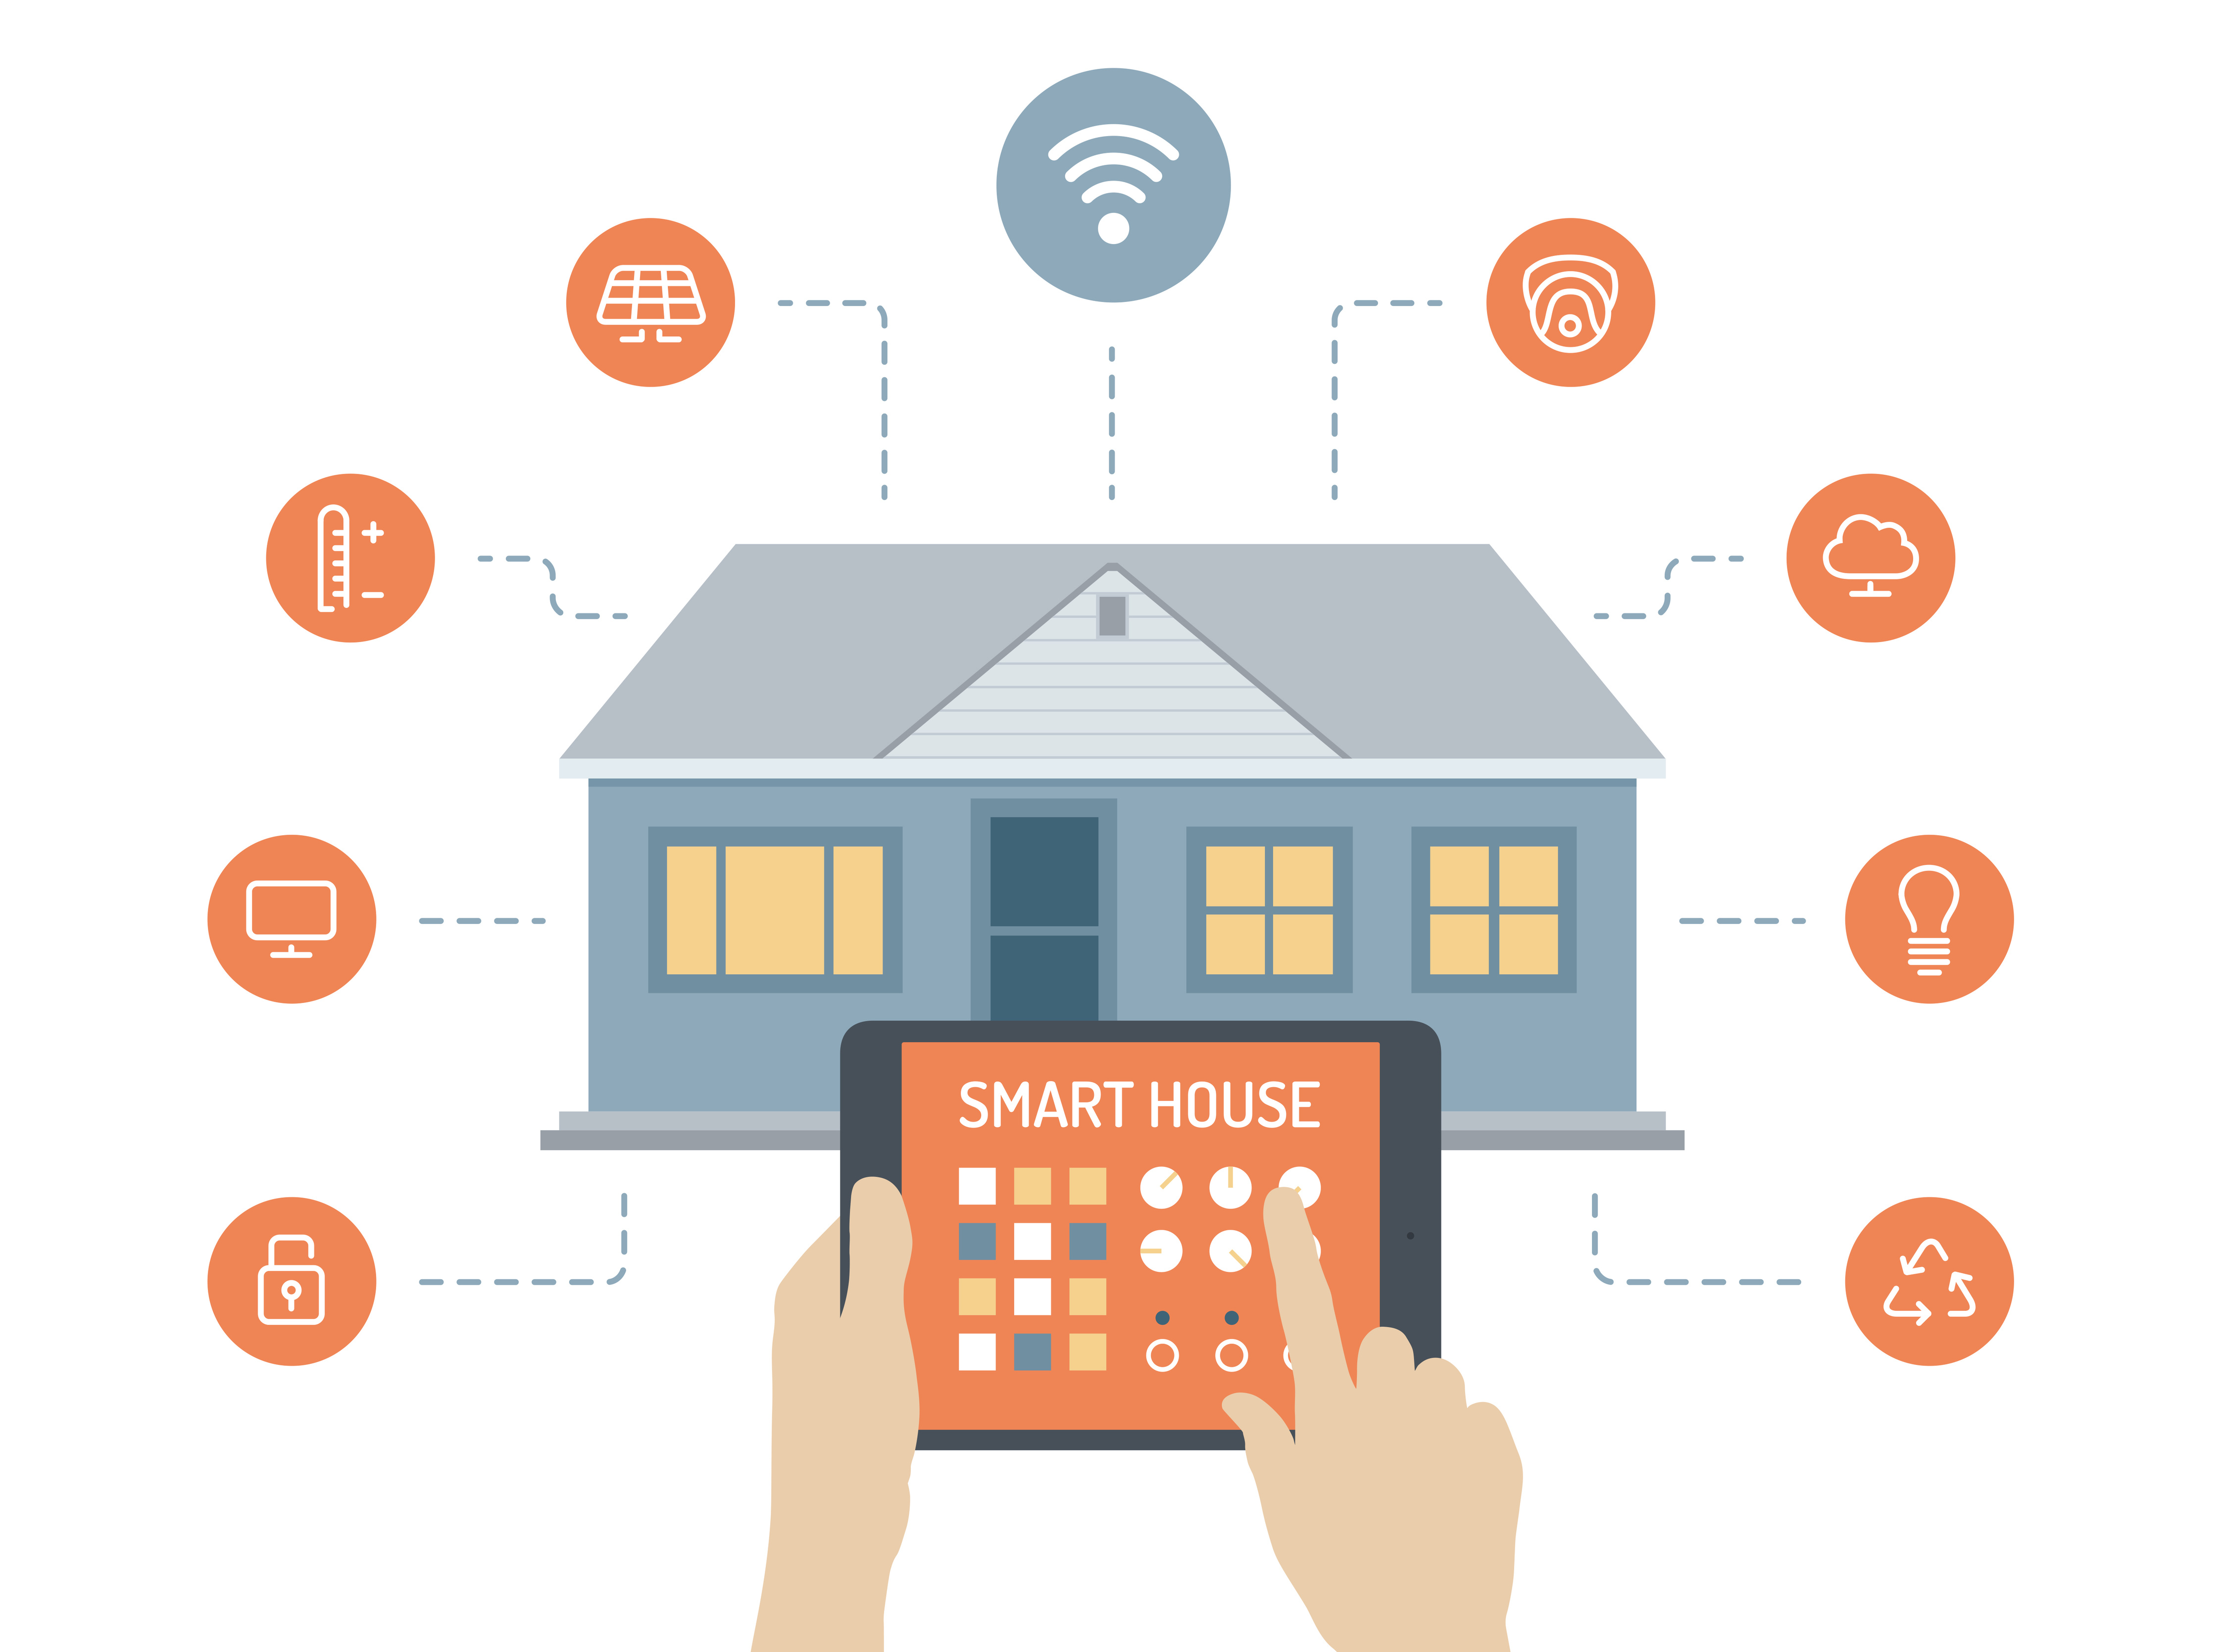
\includegraphics[width=0.6\textwidth]{SmartHome.jpg}
  \end{figure}
\end{frame}

\begin{frame}{Stuxnet}
  \begin{figure}[ht]
    \centering
    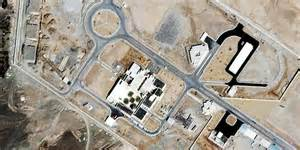
\includegraphics[width=0.8\textwidth]{stuxnet.jpg}
  \end{figure}
  Stuxnet is the first discovered malware that spies on and subverts industrial control systems. It was discovered in June 2010. 
\end{frame}

\begin{frame}{2015 Ukraine Power Outage}
  \begin{figure}[<+htpb+>]
    \begin{center}
      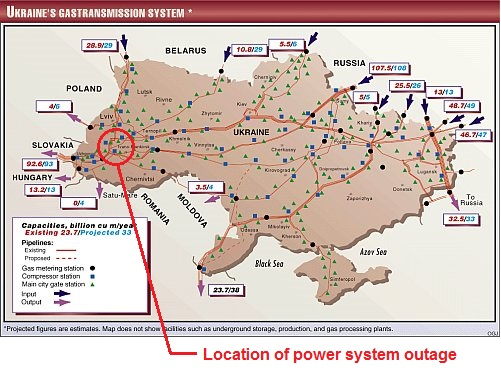
\includegraphics[width=0.60\textwidth]{ukraine.jpg}
      \caption{A successful attack on CPS can have devastating effects.}
    \end{center}
  \end{figure}
\end{frame}

\begin{frame}{Industrial Control Systems}
  \begin{figure}[ht]
    \centering
    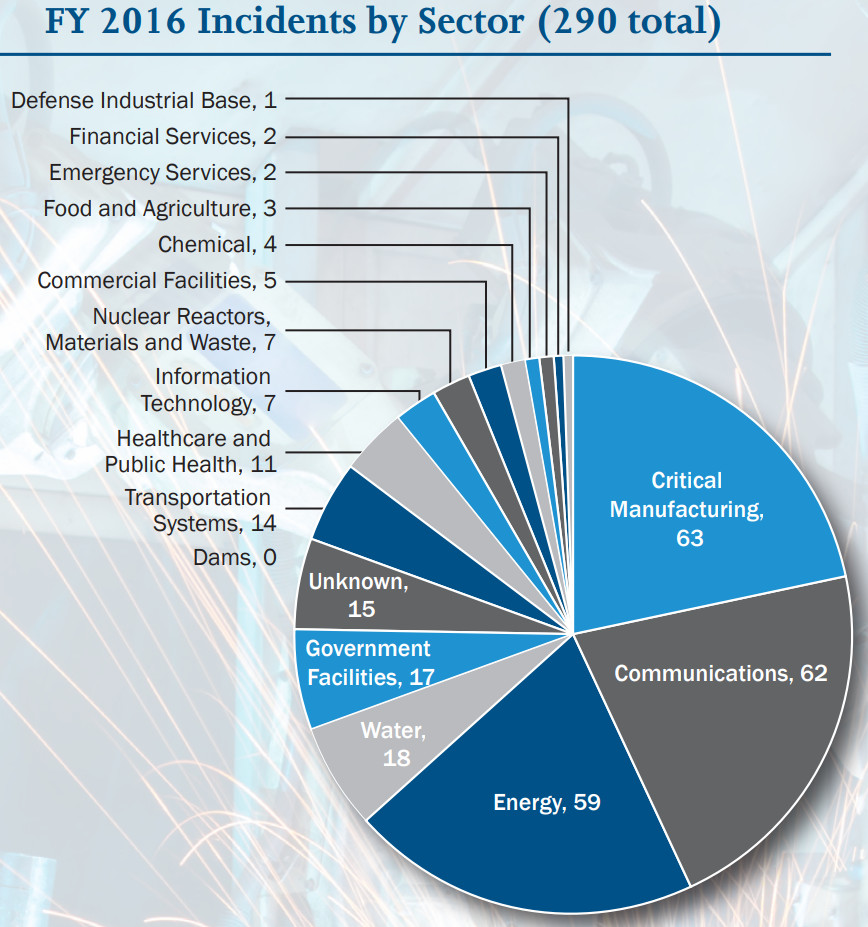
\includegraphics[width=0.55\textwidth]{cert.jpg}
  \end{figure}
  In FY 2016, ICS-CERT (Industrial Control Systems Cyber Emergency Response Team) received and responded to 290 incidents as reported by asset owners and industry partners.
\end{frame}

\begin{frame}{Industrial Control Systems}
  The scope of incidents encompassed a vast range of threats and observed methods for attempting to gain access to both business and control systems infrastructure, including but not limited to the following:
  \begin{enumerate}
    \item  Unauthorized access and exploitation of Internet facing ICS/Supervisory Control and Data Acquisition (SCADA) devices,
    \item  Exploitation of zero-day vulnerabilities in control system devices and software, 
    \item  Malware infections within air-gapped control system networks,
    \item \dots
  \end{enumerate}
\end{frame}

\begin{frame}{Attack Through Compromised Supply Chain}
  \begin{figure}[ht]
    \centering
    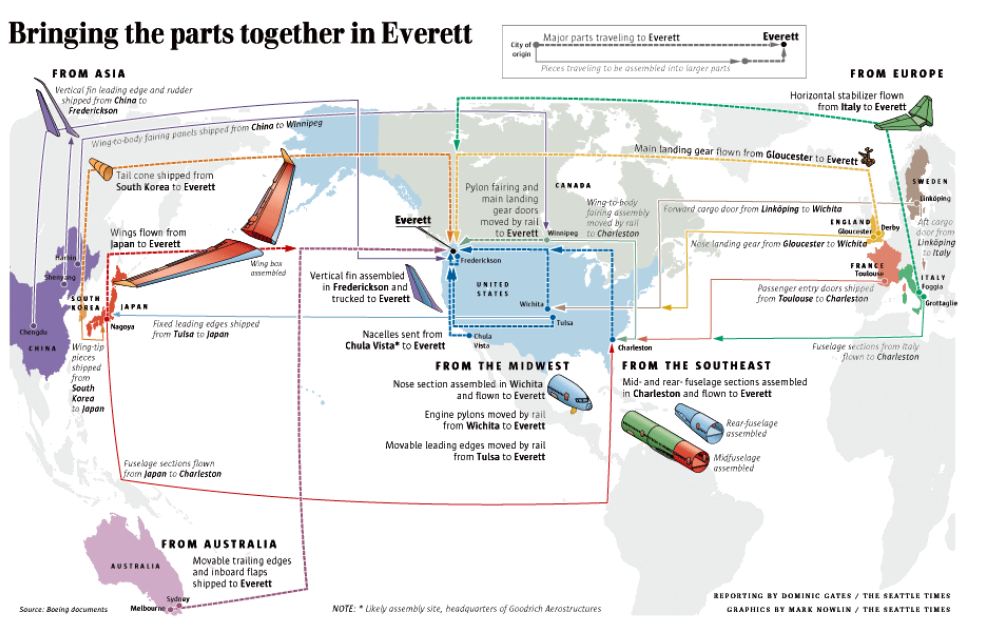
\includegraphics[width=0.8\textwidth]{boeing.jpg}
    \caption{Boeing 787 outsourced 70\% of its parts.}
  \end{figure}
\end{frame}

\begin{frame}{Hacker Taking Control of a Chrysler Jeep}
  \begin{figure}[<+htpb+>]
    \begin{center}
      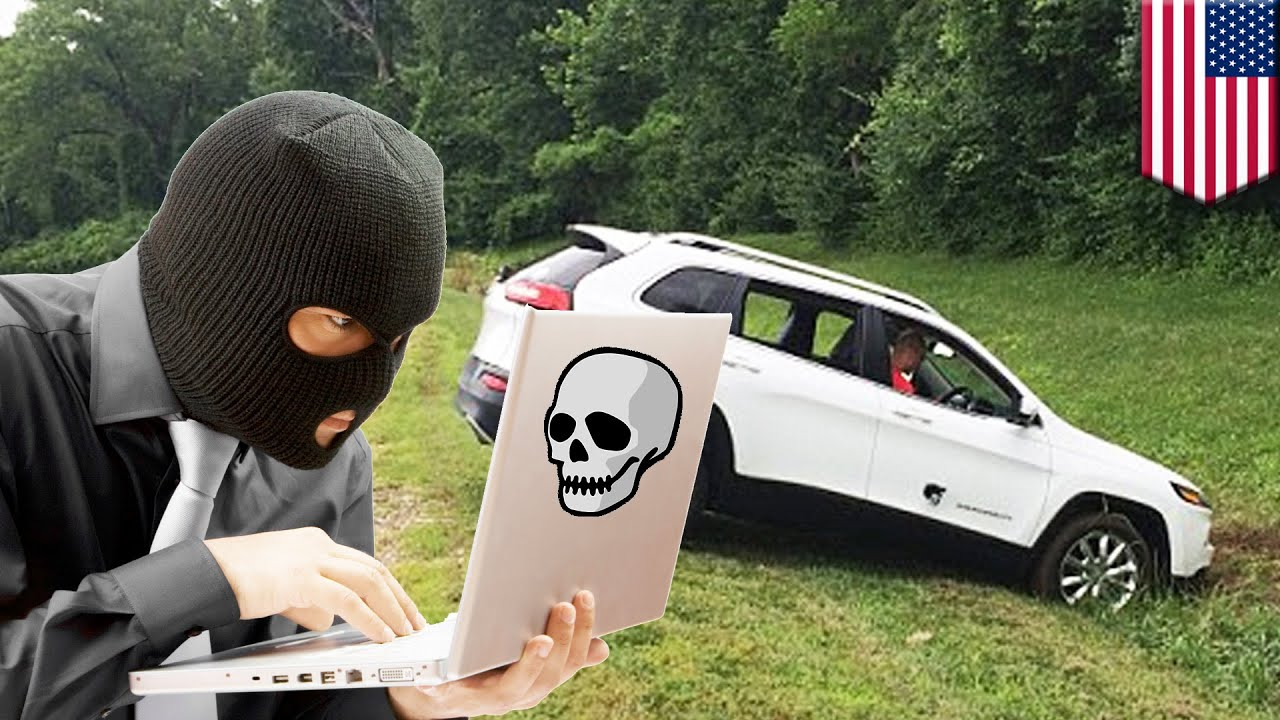
\includegraphics[width=0.80\textwidth]{jeep.jpg}
      \caption{Hacker take control of the steering and brake of a Jeep car in 2015}
    \end{center}
  \end{figure}
\end{frame}

\begin{frame}{What is New in CPS Security?}
  \begin{itemize}
    \item Physics
    \item Inertia: The system cannot be stopped at will
    \item Complicated interaction between cyber and physical world
    \item High reliability requirement: $10^{-9}$ for air plane
    \item Continuous operation, Graceful degradation.
  \end{itemize}
\end{frame}

\begin{frame}{Defense in Depth for CPS Security}
  \begin{figure}[ht]
    \centering
    \begin{tikzpicture}
      \node at (0,0) {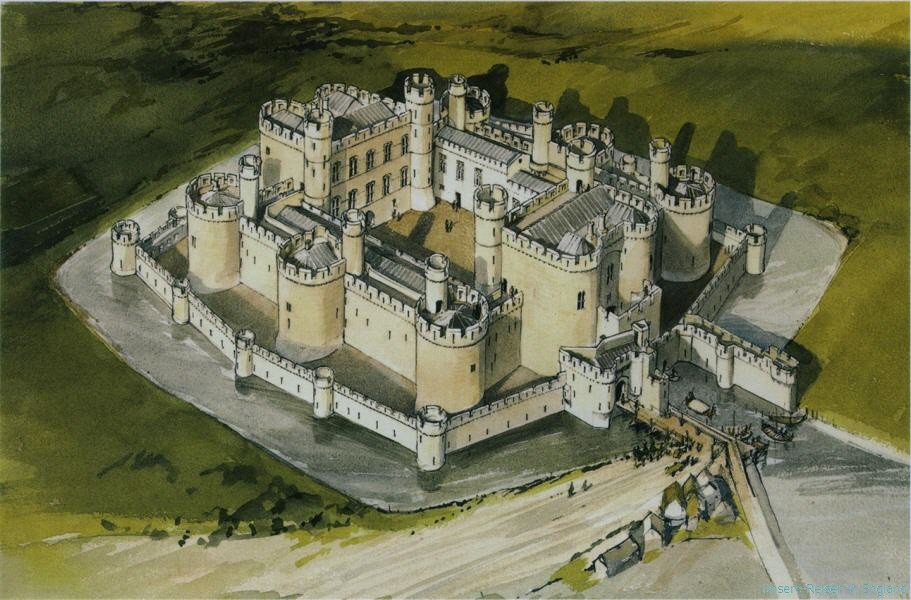
\includegraphics[width=6cm]{defense.png}};
      \node[anchor=south west] (1) at (4,1.8) {Prevention};
      \node[anchor=south west] (2) at (4,.6) {Detection};
      \node[anchor=south west] (3) at (4,-.6) {Resiliency};
      \node[anchor=south west] (4) at (4,-1.8) {Recovery};
      \draw[semithick] (2.2,0.5)--(4,1.8)--++(1.8,0);
      \draw[semithick] (2,0.4)--(4,0.6)--++(1.8,0);
      \draw[semithick] (1.2,0.6)--(4,-.6)--++(1.8,0);
      \draw[semithick] (0.2,0.7)--(4,-1.8)--++(1.8,0);
    \end{tikzpicture}
    \caption{Protecting CPS with Multi-layer Defense}
  \end{figure}
\end{frame}

\begin{frame}{What Control/System Theory Can Provide?}
  \begin{itemize}
    \item Robustness/Resiliency in off-line Design
    \item Intrusion Detection \& Isolation
    \item Secure Information Fusion/Control
    \item Security Investment
  \end{itemize}
\end{frame}

\section{Active Intrusion Detection}

\begin{frame}{Stuxnet}
  \begin{itemize}
    \item NY times:``The worm itself now appears to have included two major components. One was designed to send Iran's nuclear centrifuges spinning wildly out of control. Another seems right out of the movies: The computer program also \alert{secretly recorded what normal operations at the nuclear plant looked like, then played those readings back to plant operators}, like a pre-recorded security tape in a bank heist, so that it would appear that everything was operating normally while the centrifuges were actually tearing themselves apart.''
  \end{itemize}
\end{frame}

\begin{frame}{System Model}
  \begin{block}{System Description}
    \begin{displaymath}
      \begin{split}
	x(k+1) &= Ax(k)  + Bu(k)+w(k),\\
	y(k) &= C x(k) + v(k).
      \end{split}
    \end{displaymath}
  \end{block}
  \begin{itemize}
    \item $x(k) \in \mathbb R^n$ is the state vector.
    \item  $y(k) \in \mathbb R^m$ is the measurements from the sensors.
    \item  $u(k) \in \mathbb R^p$ is the control input.
    \item $w(k),v(k),x(0)$ are independent Gaussian random vectors, and $x(0) \sim \mathcal N(0,\;\Sigma)$, $w(k) \sim \mathcal N(0,\;Q)$ and $v(k) \sim \mathcal N(0,\;R)$ with $Q,R>0$.
    \item The system is assumed to be controllable and observable.
  \end{itemize}
\end{frame}

\begin{frame}{LQG Controller and Kalman filter}
  \begin{itemize}
    \item We assume that the system operator wants to minimize the following cost function:
      \begin{displaymath}
	J = \lim_{T\rightarrow \infty}\min_{u(0),\ldots,u(T)}E\frac{1}{T}\left[\sum_{k=0}^{T-1} x(k)'Wx(k)+u(k)'Uu(k)\right],
      \end{displaymath}
      where $W, U$ are positive semidefinite matrices. 
    \item The optimal controller is a fixed gain controller, which takes the following form:
      \begin{displaymath}
	u(k) =  L^*\hat x(k),
      \end{displaymath}
    \item The optimal estimator (Kalman filter) follows the following update equations:
      \begin{align*}
	\hat x(k+1|k) &= A\hat x(k)+Bu(k),\\
	\hat x(k+1) &= \hat x(k+1|k) + K^*\left[y(k+1) - C\hat x(k+1|k)\right],
      \end{align*}
  \end{itemize}
\end{frame}

\begin{frame}{$\chi^2$ Failure Detector}
  \begin{itemize}
    \item The residue $z(k)$ of the Kalman filter is defined as
      \begin{displaymath}
	z(k) \triangleq y(k) - C\hat x(k|k-1),
      \end{displaymath} 
      which is i.i.d. Gaussian distributed with zero mean. 
    \item $\chi^2$ detector triggers an alarm based on the following event:
      \begin{displaymath}
	g(k)=  z(k)^T\mathcal P^{-1}z(k)> threshold,
      \end{displaymath}
      where $\mathcal P$ is the covariance matrix of $z(j)$ and $\mathcal T$ is the window size.
    \item The alarm rate at time $k$ is 
      \begin{displaymath}
	\beta(k) = P(g(k) > threshold).
      \end{displaymath}
      If the system is operating normally, then the alarm rate is a constant, which we denote as the false alarm rate $\alpha$.
  \end{itemize}
\end{frame}

\begin{frame}{System Diagram}
  \begin{figure}[htpb]
    \begin{center}
      \inputtikz{systemdiagram}
    \end{center}
  \end{figure}
  Assumptions: Linear System, Kalman Filter, LQG controller and $\chi^2$ detector.
\end{frame}

\begin{frame}{Replay Attack Model}
  \begin{enumerate}
    \item The attacker can read and modify all the measurements $y(k)$ arbitrarily.
    \item It can inject an external control input $u^a(k)$ into the system. 
  \end{enumerate}
  The strategy of the attacker can be divided into two stages:
  \begin{enumerate}
    \item The attacker records a sufficient number of $y(k)$s without injecting any control input $u^a(k)$. 
    \item The attacker injects a sequence of desired control input $u^a(k)$ while replaying the previous recorded $y(k)$s starting from time $0$.
  \end{enumerate}
  When the system is under attack, the controller will be unable to perform closed-loop control. Hence the only way to counter this attack is to detect its presence. 
\end{frame}

\begin{frame}{Replay Attack: First Stage}
  \begin{figure}[htpb]
    \begin{center}
      \inputtikz{replaydiagramone}
    \end{center}
  \end{figure}
\end{frame}

\begin{frame}{Replay Attack: Second Stage}
  \begin{figure}[htpb]
    \begin{center}
      \inputtikz{replaydiagramtwo}
    \end{center}
  \end{figure}
\end{frame}

\begin{frame}{Feasibility of Replay Attacks}
  \begin{figure}[htpb]
    \setlength\figureheight{4.5cm}
    \setlength\figurewidth{10cm}
    \begin{center}
      \inputtikz{replayunstableA2}
    \end{center}
  \end{figure}
  Replay attack is not always feasible!
\end{frame}

\begin{frame}{Feasibility of Replay Attacks}
  \begin{figure}[htpb]
    \begin{center}
      \inputtikz{replaydiagramthree}
    \end{center}
  \end{figure}
\end{frame}

\begin{frame}{Feasibility of Replay Attacks}
  The update equation of Kalman filter follows:
  \begin{align*}
    \hat{x}(k+1|k)&=A\hat{x}(k)+Bu(k)=\left(A+BL^*\right)\hat{x}(k)\\
		  &=\left(A+BL^*\right)\left(I-K^*C\right)\hat{x}(k|k-1)+\left(A+BL^*\right)K^*y(k).
  \end{align*}

  \begin{theorem}
    If $\mathcal A = (A+BL^*)(I-K^*C)$ is stable, then the detection rate of $\chi^2$ detector $\beta^c(k)$ converges to the false alarm rate $\alpha$ during the attack, i.e.,
    \begin{displaymath}
      \lim_{k\rightarrow\infty}\beta^c(k) = \alpha.  
    \end{displaymath}
    On the other hand, if $\mathcal A$ is strictly unstable, then the detection rate $\beta^c(k)$ converges to $1$, i.e.,
    \begin{displaymath}
      \lim_{k\rightarrow\infty}\beta^c(k) = 1.  
    \end{displaymath}
  \end{theorem}
\end{frame}

\begin{frame}{Countermeasures: Authentication via Watermarking}
  \begin{itemize}
    \item We could change the control law by adding a random watermarking signal:
      \begin{displaymath}
%	u(k) = \text{Optimal LQG Control}+ \zeta(k).
	u(k) = \text{Optimal Control}+ \zeta(k).
      \end{displaymath}
    \item The watermarking signal $\zeta(k)$ acts as a ``challenge'' and the sensor measurement is the ``response''. 
    \item During normal operation, the ``challenge'' and ``response'' are correlated through the system dynamics, while the correlation cease to exist when the replay begins.
%    \item The CPS will remain stable. However, we sacrifice LQG performance since the control is not optimal.
    \item Optimize detection and minimize disturbance
  \end{itemize}
\end{frame}

\begin{frame}{System with Physical Watermarks}
  \begin{figure}[htpb]
    \begin{center}
      \inputtikz{replaywithphywatermark}
    \end{center}
  \end{figure}
\end{frame}

\begin{frame}{Active Detection of Replay Attack}
  \setlength{\figureheight}{6cm}
  \setlength{\figurewidth}{7cm}
  \begin{figure}[htpb]
    \begin{center}
      \inputtikz{replay1}
    \end{center}
  \end{figure}
\end{frame}

\begin{frame}{Detection Performance v.s. Control Performance}
  \begin{itemize}
    \item Assuming the watermarking signal is i.i.d. zero mean Gaussian with covariance $U$.
    \item The optimal watermarking signal design problem can be written as
      \begin{align*}
      &\mathop{\textrm{maximize}}\limits_{U\geq 0}&
      & Detection\;Performance\\
      &\textrm{subject to}&
      & Additional\;LQG\;Cost \leq \delta.
      \end{align*}
    \item The above problem can be relaxed into an Semi-Definite Programming problem. The optimal solution can be derived analytically using generalized eigenvectors.
  \end{itemize}
\end{frame}
%
%\begin{frame}{Stationary Watermarking}
%  \begin{itemize}
%    \item We can consider a zero mean stationary Gaussian signal, with autocovariance function:
%      \begin{align*}
%	\Gamma(d) = \mathbb E \zeta(k)\zeta(k+d)^T.
%      \end{align*}
%    \item All autocovariance functions form a convex cone.
%    \item The optimal trade-off is attained at the boundary of the cone, consisting of signals of the following form: 
%      \begin{align*}
%        \zeta(k) = H \xi(k),
%      \end{align*}
%      where $\xi(k)\in \mathbb R^2$ is a hidden state satisfies:
%      \begin{align*}
%      \xi(k+1) = \begin{bmatrix}
%	  \cos 2\pi\omega & -\sin 2\pi\omega \\
%	  \sin 2\pi\omega & \cos 2\pi\omega \\
%	\end{bmatrix} \xi(k).
%      \end{align*}
%  \end{itemize} 
%\end{frame}

\subsection{An Online Approach to Replay Attack Detection}

\begin{frame}{Data-Driven Approach}
  \begin{figure}[htpb]
    \inputtikz{systemdiagram2}
  \end{figure}
\end{frame}

\begin{frame}{Modified System Model}
  \begin{figure}
    \centering
    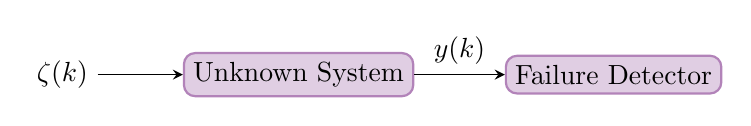
\begin{tikzpicture}
      \node (p1) at (0,0) {$\zeta(k)$};
      \node [draw=thupurple!50,fill=thupurple!20,thick,rounded corners] (p2) at (3,0) {Unknown System};
      \node [draw=thupurple!50,fill=thupurple!20,thick,rounded corners] (p3) at (7,0) {Failure Detector};
      \draw [semithick,-stealth] (p1)--(p2);
      \draw [semithick,-stealth] (p2)--node[above]{$y(k)$} (p3);
    \end{tikzpicture}
  \end{figure}
  \begin{enumerate}
    \item System Dynamics:
      \begin{align*}
	x(k+1) = A x(k) + B\zeta(k)+w(k), \;y(k)  &= C x(k) + v(k) . 
      \end{align*}
    \item LQG cost:
      \begin{align*}
	J = \lim_{T \to +\infty} \mathbb E\left [\frac{1}{T}\sum_{k=0}^{T-1} \begin{bmatrix}
	    y(k)\\
	    \zeta(k)
	    \end{bmatrix}^TX \begin{bmatrix}
	    y(k)\\
	    \zeta(k)
	\end{bmatrix} \right ],
      \end{align*}
  \end{enumerate}
\end{frame}

\begin{frame}{Assumptions}
  \begin{itemize}
    \item The system is stable (or has been stabilized by some inner-loop controller), controllable and observable.
    \item $A$ is diagonalizable.
    \item We can observe $y(k)$, and we know the dimension of the $x(k)$.
    \item The LQG weight matrix $X$ is known.
    \item The noise are all zero mean i.i.d. Gaussian.
  \end{itemize}
  \textbf{No additional knowledge} on the $A,B,C$ matrices or the covariance of the noise is assumed.
\end{frame}
%
\begin{frame}{Impact on the Control Performance}
  The additional LQG cost incurred by the watermarking signal is a linear function of $U$.
  \begin{displaymath}
    \text{Additional LQG cost} = \tr(U\mathcal X).
  \end{displaymath}
  where $\mathcal X$ is given by:
  \begin{align*}
    \mathcal X &\triangleq \sum_{k=0}^\infty\textcolor{thupurple}{\left(CA^kB\right)^T} X_{yy}\textcolor{thupurple}{\left(CA^kB\right)}+ \textcolor{thupurple}{\left(CB\right)^T}X_{y\phi} + X_{\phi y}\textcolor{thupurple}{CB}+ X_{\phi \phi}\\
	       &= \sum_{k=0}^\infty \textcolor{thupurple}{H_k^T} X_{yy}\textcolor{thupurple}{H_k}+ \textcolor{thupurple}{H_0^T}X_{y\phi} + X_{\phi y}\textcolor{thupurple}{H_0}+ X_{\phi \phi}.
  \end{align*}
\end{frame}
%
%
\begin{frame}{Detecting Replay Attacks}
  \begin{itemize}
    \item In the absence of the attack:  
      \begin{align*} 
	y(k) &=\textcolor{red}{\boxed{\sum_{t=0}^{k-1} CA^{t}B  \zeta(k-1-t)}} + \textcolor{blue}{\boxed{\sum_{t=0}^{k-1}  CA^{t} w(k-1-t)+v(k) }}\\ 
	     &=\textcolor{red}{\gamma(k-1)} +\textcolor{blue} {\vartheta(k-1)},
      \end{align*}
    \item  In the presence of the attack:
      \begin{align*}
	y^c(k) = y(k-\Delta k) = \textcolor{red}{\gamma(k-1-\Delta k)} + \textcolor{blue}{\vartheta(k-1-\Delta k)}.
      \end{align*}
    \item The KL divergence between ``compromised'' measurement $y^c(k)$ and ``normal'' measurement $y(k)$ is a convex function $U$:
      \begin{displaymath}
	\tr\left( U \mathcal P  \right) - \frac{1}{2}\logdet\left( I+ U \mathcal P \right),
      \end{displaymath}
      where
      \begin{align*}
	\mathcal P \triangleq\sum_{k=0}^\infty \textcolor{thupurple}{H_k^T\mathcal W^{-1}H_k},\\
      \end{align*}
      where $\mathcal W$ is the covariance of $\vartheta_{k-1}$.
  \end{itemize}
\end{frame}

\begin{frame}{Optimal Watermark}
  \begin{block}{Problem 1}
    \begin{align*}
      &\mathop{\textrm{maximize}}\limits_{U}&
      & \tr\left( U \mathcal P  \right) - \frac{1}{2}\logdet\left( I+ U \mathcal P \right), \\
      &\textrm{subject to}&
      & \tr (U\textcolor{thupurple}{\mathcal X}) \leq \delta \\
      &&& U \text{ is positive semidefinite.}
    \end{align*}
  \end{block}
  \centering
  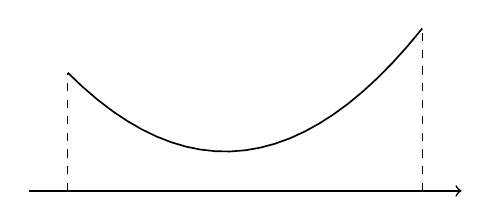
\begin{tikzpicture}[domain=-2:2.5]
    \draw[semithick] plot (\x,{\x*\x/4});
    \draw[semithick,->] (-2.5,-0.5)--(3,-0.5);
    \draw[dashed] (-2,-0.5)--(-2,1);
    \draw[dashed] (2.5,-0.5)--(2.5,1.5625);
  \end{tikzpicture}

  The solution lies on the boundary of the feasible set!
\end{frame}

\begin{frame}{Optimal Watermark}
  \begin{enumerate}
    \item The boundary of the set of positive semi-definite matrices are rank $1$ matrix:
      \[U = \alpha vv^T.\] 
    \item $v$ is the generalized eigenvector s.t. $\mathcal Pv = \lambda\mathcal Xv$, where $\lambda$ is the largest generalized eigenvalue.
    \item $\alpha$ is chosen such that $\tr(U\mathcal X)=\delta$.
  \end{enumerate}
\end{frame}

\begin{frame}{Online-Watermark Design}
  \begin{figure}[t]
    \centering
    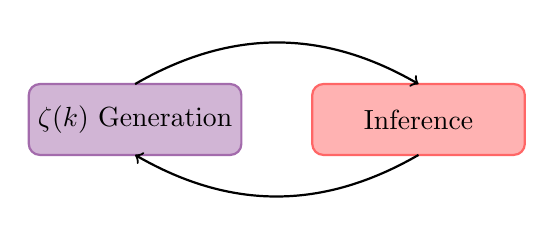
\begin{tikzpicture}[scale=0.9]
      \draw[thick,rounded corners,fill=thupurple!30,draw=thupurple!60] (0,1) rectangle (3,2);
      \node at (1.5,1.5) {$\zeta(k)$ Generation};
      \draw[thick,rounded corners,fill=red!30,draw=red!60] (4,1) rectangle (7,2);
      \node at (5.5,1.5) {Inference};
      \draw[thick,->] (1.5,2) to [bend left] (5.5,2);
      \draw[thick,->] (5.5,1) to [bend left] (1.5,1);
    \end{tikzpicture}
  \end{figure}
  \begin{itemize}
    \item Generate the ``optimal'' $U$ (based on our current knowledge):
      \begin{align*}
	\hat U_k=&\mathop{\textrm{argmax}}\limits_{U\geq 0}&
		 & \tr (U\textcolor{thupurple}{\hat  P_k})\\
		 &\textrm{subject to}&
		 & \tr (U\textcolor{thupurple}{\hat  X_k}) \leq \delta.
      \end{align*}
    \item Generate the watermark signal:
      \begin{align*}
	\zeta(k) = \left(\hat U_k+k^{-\beta}I\right)^{1/2}\phi(k),\,where\; \phi(k)\sim\mathcal N(0,I).
      \end{align*}
    \item Update the estimated system parameters using the cross correlation between $y$ and $u$.
  \end{itemize}
\end{frame}
%
%\begin{frame}{Online-Watermark Design: Inference}
%  \begin{figure}[t]
%    \centering
%    \begin{tikzpicture}[scale=0.9]
%      \draw[thick,rounded corners,fill=thupurple!30,draw=thupurple!60] (0,1) rectangle (3,2);
%      \node at (1.5,1.5) {$\zeta(k)$ Generation};
%      \draw[thick,rounded corners,fill=red!30,draw=red!60] (4,1) rectangle (7,2);
%      \node at (5.5,1.5) {Inference};
%      \draw[thick,->] (1.5,2) to [bend left] (5.5,2);
%      \draw[thick,->] (5.5,1) to [bend left] (1.5,1);
%    \end{tikzpicture}
%  \end{figure}
%  \begin{itemize}
%  \item If we compute $y(k)\phi(k)^T$, we get
%    \begin{align*}
%      y(k+1)\phi(k)^T &= \textcolor{thupurple}{CBU_k^{1/2}\phi(k)\phi(k)^T}+ \sum_{t=1}^{k}H_t U_{k-t}^{1/2} \phi(k-t) \phi(k)^T \\
%                      &+\sum_{t=0}^{k}  CA^{t} w(k-t)\phi(k)^T +v(k+1)\phi(k)^T.
%    \end{align*}
%  \item One tentative way to infer $H_0$: 
%    \begin{align*}
%      H_0 \approx \text{the average of }y(k+1)\phi(k)^TU_{k}^{-1/2} . 
%    \end{align*}
%  \item Similarly we can estimate all $H_t$, and further infer $\mathcal P$ and $\mathcal X$.
%  \end{itemize} 
%\end{frame}
%
%\begin{frame}{Key Problems with the Naive Approach}
%  \begin{itemize}
%  \item There are infinitely $H_t$s we need to infer
%  \item The ``optimal'' $U_k$ is rank 1 and not invertible
%  \end{itemize}
%\end{frame}
%\begin{frame}{Infer all $H_t$ using finitely many $H_t$s}
%  \begin{itemize}
%  \item We can only store \textbf{finitely many} $H_t=CA^tB$s, but we need \textbf{all} $H_t$ to compute $\mathcal P$ and $\mathcal X$.
%  \item Solution: Cayley-Hamilton Theorem: 
%    \begin{align*}
%      p(A) = A^n + \alpha_{n-1}A^{n-1}+\ldots+\alpha_1 A + \alpha_0 I = 0     
%    \end{align*}
%    where $p(x)$ is the characteristic polynomial of $A$. 
%  \item As a result, we know that
%    \begin{align*}
%      H_{n+i} &+ \alpha_{n-1}H_{n-1+i}+\ldots+\alpha_0 H_i\\
%              &= CA^{i}A^nB + \alpha_{n-1}CA^{i}A^{n-1}B+\ldots+\alpha_0 CA^iB\\
%      &=CA^i p(A)B = 0.
%    \end{align*}
%    \item All $H_\tau$ can be deduced from $H_0,\ldots, H_{n-1}$, if we know $p(A)$.
%    \item Actually as long as we know some non-trivial polynomial $\tilde p(x)$, such that $\tilde p(A) = 0$, we can deduce all $H_\tau$ from finitely many $H_\tau$s.
%  \end{itemize} 
%\end{frame}
%
%\begin{frame}{Infer the Characteristic Polynomial $p(A)$}
%  \begin{itemize}
%  \item Suppose that we find some coefficients $\tilde \alpha_i$, such that
%    \begin{align*}
%      H_{n+i} &+ \tilde \alpha_{n-1}H_{n-1+i}+\ldots+\tilde \alpha_0 H_i = 0.
%    \end{align*}
%  \item Let $\tilde p(x) = x^n + \alpha_{n-1}x^{n-1}+\ldots+\alpha_1 x + \alpha_0 $.
%  \item Question: Under what condition, will $\tilde p(x) = 0$?
%  \item $CA^i\tilde p(A)B = 0$ for $i=0$ to $2n-2$, then
%    \begin{align*}
%      \begin{bmatrix}
%        C\\
%        CA\\
%        \cdots\\
%        CA^{n-1}
%      \end{bmatrix}\tilde p(A)\begin{bmatrix}
%        B&AB&\cdots&A^{n-1}B
%      \end{bmatrix}=0.
%    \end{align*}
%  \item If the system is controllable and observable, then $\tilde p(A)=0$. 
%    
%  \end{itemize} 
%\end{frame}
%
\begin{frame}{Exploration and Exploitation}
  \begin{figure}[ht]
    \centering
    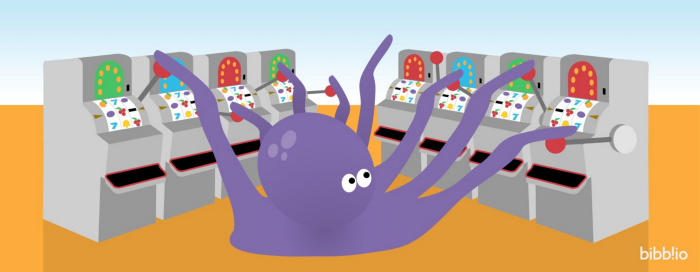
\includegraphics[width=0.8\textwidth]{bandit.png}
    \caption{Multi-Armed Bandit}
  \end{figure}
\end{frame}

\begin{frame}{Balance Exploration and Exploitation}
  \begin{itemize}
    \item The solution of the optimization problem is a rank one matrix: Pure \textcolor{red}{Exploitation}.
    \item We could also consider classical system identification techniques, which use $\hat U_k=I$: Pure \textcolor{blue}{Exploration}.
    \item To achieve a balance, choose
      \begin{align*}
	\hat U_k = \text{``optimal'' } U + k^{-\beta} I.
      \end{align*}
    \item More \textcolor{blue}{exploration} at the beginning and more \textcolor{red}{exploitation} towards the end.
  \end{itemize}
\end{frame}

\begin{frame}{Convergence of the Watermarking Signal}
  \begin{theorem}
    If $0 \leq \beta < 1$, then $\hat U_k$ converges to the optimal $U$ a.s. Furthermore, for any $\epsilon > 0$, we have
    \begin{align*}
      \frac{\hat U_k - U}{k^{-1/2+\beta/2+\epsilon}} \rightarrow 0,\,a.s.
    \end{align*}
  \end{theorem}
\end{frame}

\begin{frame}{Tennessee Eastman Process}
  The TEP is created to provide a realistic industrial process for developing studying and evaluating process control technology. 
  \begin{columns}
    \begin{column}{0.45\textwidth}
      \begin{figure}
	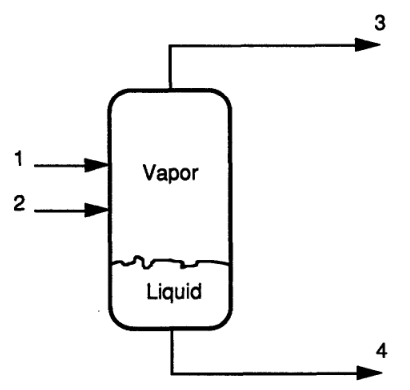
\includegraphics[width=0.9\textwidth]{simplifiedmodel.png}
	\caption{The simplified process}
      \end{figure}
    \end{column}
    \begin{column}{0.55\textwidth} 		
      \begin{itemize}
	\item The vessel: a combination of the reactor and separation system in the original TE Process;
	\item Feed 1: A, C and trace amounts of an inert B;
	\item Feed 2: pure A;
	\item Stream 3: purge rate;
	\item Stream 4: product rate;
	\item Vapor: A, B, C;\\
	  Liquid: D.
      \end{itemize}
    \end{column}
  \end{columns}
  4 inputs, 4 outputs and 7 internal states.
\end{frame}

\begin{frame}
  \frametitle{The Watermark Signal Design}
  \begin{columns}
    \begin{column}{0.6\textwidth}
      \begin{figure}[h!]
	\inputtikz{errU1_te}
      \end{figure}
    \end{column}
    \begin{column}{0.4\textwidth}
      \begin{itemize}
	\item $U$: the optimal covariance of the watermark signal;
	\item $U_k$: the estimation of $U$.
      \end{itemize}
    \end{column}
  \end{columns}
  ~\\
  As time $k$ goes to infinity, $U_k$ converges to the optimal covariance of the watermark signal, $U$.
\end{frame}

\begin{frame}{The detection performance}
  \begin{itemize}
    \item $g$: the output of the failure detector designed with know parameters
    \item $\hat g$: the output of the failure detector when the parameters of the system are inferred through the learning technique. 
  \end{itemize}
  \begin{figure}[h!]
    \centering
    \inputtikz{gng_te}
  \end{figure}
\end{frame}

\section{Secure State Estimation}
\subsection{Static State Estimation}

\begin{frame}{Problem Formulation}
  \begin{enumerate}
    \item We assume the following sensor model:
      \begin{align*}
	\begin{bmatrix}z_1\\\vdots\\z_m\end{bmatrix} =  z = Hx + w.
      \end{align*}
    \item The optimal state estimator is of the form
      \begin{align*}
	\hat x = Kz, \text{ where }K = (H^TH)^{-1}H^T.
      \end{align*}
  \end{enumerate}
\end{frame}

\begin{frame}{Least Square Estimator}
  Suppose the following sensory model:
  \begin{align*}
    z = \begin{bmatrix}
      1\\
      1\\
      1
    \end{bmatrix}x + w.
  \end{align*}
  The optimal estimator is given by
  \begin{align*}
    \hat x = \frac{1}{3}\left(z_1+z_2+z_3\right).
  \end{align*}
  This estimator is not resilient to a single malicious sensor.
\end{frame}

\begin{frame}{Problem Formulation}
  \begin{enumerate}
    \item Assume that at most $c$ sensors are compromised.
    \item The sensory model is given by
      \begin{align*}
	y = z + a = Hx + w +a,
      \end{align*}
      where $a$ is a $c$-sparse vector indicating the attacker's action.
    \item We will call an estimator $\hat x = g(y)$ to be resilient if
      \begin{align*}
	\|g(y) - g(z)\|\text{ is bounded for all $c$-sparse $a$}.
      \end{align*}
  \end{enumerate}
\end{frame}

\begin{frame}{Some Related Research}
  \begin{enumerate}
  \item The following estimator is resilient under $2c$ observable condition:
    \begin{align*}
      & \mathop{\textit{minimize}}\limits_{\hat x,a,w}&
      & \|w\|^2 \\
      &\text{subject to}&
      &y = H \hat x + w + a,\,\|a\|_0\leq p.
    \end{align*}
  \item Difficult to verify $2c$ observable condition and difficult to solve
\item The secure estimation problem for general system is proved to be NP hard\footcite{Hendrickx2014}\footcite{Mao2019}.
  \item Can we design a secure and computationally efficient estimators for {\bf some} system?
  \end{enumerate}
\end{frame}

\begin{frame}{Example}
  Suppose the following sensory model:
  \begin{align*}
    y = \begin{bmatrix}
      1\\
      1\\
      1
    \end{bmatrix}x + w+a,\,\|a\|_0\leq 1.
  \end{align*}
  \begin{itemize}
   \item The mean is not resilient: 
  \begin{align*}
    g(y) = \argmin_{\hat x}  (y_1-\hat x)^2+(y_2-\hat x)^2+(y_3-\hat x)^2.
  \end{align*}
    \item The median is resilient to one malicious sensor.
    \item Moreover, the median can be viewed as the solution for the following optimization problem. 
  \begin{align*}
    g(y) = \argmin_{\hat x}  |y_1-\hat x|+|y_2-\hat x|+|y_3-\hat x|.
  \end{align*}
  \end{itemize}
\end{frame}

\begin{frame}{Example}
  \begin{figure}[ht]
    \centering
    \begin{tikzpicture}[yscale=0.4]
      \draw[thick,->] (0,0)--(9,0);
      \node [anchor=west] at (9,0) {$\hat x$};
      \draw[thin,gray] (2,0)--(2,0.1);
      \draw[thin,gray] (5,0)--(5,0.1);
      \draw[thin,gray] (7,0)--(7,0.1);
      \draw[thick](1,11)--(2,8)--(5,5)--(7,7)--(8,10);
      \node [anchor=north] at (2,0) {\color{red}{$y_1$}};
      \node [anchor=north] at (5,0) {\color{blue}{$y_2$}};
      \node [anchor=north] at (7,0) {\color{brown}{$y_3$}};
    \end{tikzpicture}
  \end{figure}
\end{frame}

\begin{frame}{A General Convex Optimization Based Estimator}
  We consider the following estimator
  \begin{align*}
    \hat x = g(y) \triangleq \argmin_{\hat x} \sum_{i=1}^m f_i(y_i-H_i \hat x),
  \end{align*}
  where the following properties of function $f_i:\mathbb R\mapsto \mathbb R$ are assumed:
  \begin{enumerate}
    \item $f_i$ is convex.
    \item $f_i$ is symmetric, i.e., $f_i(u) = f_i(-u)$.
    \item $f_i$ is non-negative and $f_i(0) = 0$.
  \end{enumerate} 

  Many estimators, such as least square estimator, L1 estimator and LASSO estimation can be included in this framework, by choosing a suitable $f_i$.

  The estimator can be computed efficiently via convex optimization. 
\end{frame}

\begin{frame}{A General Convex Optimization Based Estimator}
  Our proposed estimator is very general since we can choose the right $f_i$ to get the following estimator:
  \begin{enumerate}
  \item Least Square Estimator:
    \begin{align*}
      g(y) = \argmin_{\hat x} \|y-H\hat x\|_2^2= \argmin_{\hat x}  \sum_{i=1}^m (y_i-H_i\hat x)^2.
    \end{align*}
  \item $L_1$ Estimator:
    \begin{align*}
      g(y) = \argmin_{\hat x} \|y-H\hat x\|_1=\argmin_{\hat x} \sum_{i=1}^m |y_i-H_i\hat x|.
    \end{align*}
  \end{enumerate}
\end{frame}

\begin{frame}{A General Convex Optimization Based Estimator}
  \begin{enumerate}  \setcounter{enumi}{2}
  \item LASSO:
    \begin{align*}
      g(y) = \argmin_{\hat x} \|w\|^2+\gamma \|a\|_1, \text{ s.t. }y=H\hat x+w+a.
    \end{align*}
    After some manipulations, we can rewrite the optimization problem as
    \begin{align*}
      g(y) = \argmin_{\hat x} \sum_{i=1}^m f(y_i-H_i\hat x)
    \end{align*}
    where $f$ is the Huber loss function:
    \begin{align*}
      f(r) = \min_{w} w^2 + \gamma |r-w| = \begin{cases}
        r^2 & \text{if } r \leq \gamma/2\\
        \gamma |r|-\gamma^2/4 & \text{if } r\geq \gamma/2\\
      \end{cases}.
    \end{align*}
    \begin{itemize}
    \item Quadratic when the residue is small
    \item Linear when the residue is large
    \item The quadratic region is controlled by $\gamma$.
    \item We will leverage it to design an estimator that is both secure and efficient.
    \end{itemize}
  \end{enumerate}
\end{frame}

\begin{frame}{Huber Loss Function}
  \begin{figure}[ht]
    \begin{center}
      \definecolor{color0}{rgb}{0.886274509803922,0.290196078431373,0.2}
      \definecolor{color1}{rgb}{0.203921568627451,0.541176470588235,0.741176470588235}
      \setlength{\figureheight}{6cm}
      \setlength{\figurewidth}{10cm}
      % 
      \begin{tikzpicture}
	\begin{axis}[
	  width=\figurewidth,
	  height=\figureheight,
	  axis background/.style={fill=white!89.8039215686275!black},
	  axis line style={white},
	  tick align=outside,
	  tick pos=left,
	  x grid style={white},
	  xlabel={residue $r$},
	  ylabel={$f(r)$},
	  xmajorgrids,
	  xmin=-2.2, xmax=2.2,
	  xtick style={color=white!33.3333333333333!black},
	  y grid style={white},
	  ymajorgrids,
	  ymin=-0.15, ymax=3.15,
	  ytick style={color=white!33.3333333333333!black}
	  ]
	  \addplot [ultra thick, color0]
	    table[row sep=crcr]{%
	      -1 1\\
	      -0.98 0.9604\\
	      -0.96 0.9216\\
	      -0.94 0.8836\\
	      -0.92 0.8464\\
	      -0.9 0.81\\
	      -0.88 0.7744\\
	      -0.86 0.7396\\
	      -0.84 0.7056\\
	      -0.82 0.6724\\
	      -0.8 0.64\\
	      -0.78 0.6084\\
	      -0.76 0.5776\\
	      -0.74 0.5476\\
	      -0.72 0.5184\\
	      -0.7 0.49\\
	      -0.68 0.4624\\
	      -0.66 0.4356\\
	      -0.64 0.4096\\
	      -0.62 0.3844\\
	      -0.6 0.36\\
	      -0.58 0.3364\\
	      -0.56 0.3136\\
	      -0.54 0.2916\\
	      -0.52 0.2704\\
	      -0.5 0.25\\
	      -0.48 0.2304\\
	      -0.46 0.2116\\
	      -0.44 0.1936\\
	      -0.419999999999999 0.1764\\
	      -0.399999999999999 0.16\\
	      -0.379999999999999 0.1444\\
	      -0.359999999999999 0.1296\\
	      -0.339999999999999 0.1156\\
	      -0.319999999999999 0.1024\\
	      -0.299999999999999 0.0899999999999996\\
	      -0.279999999999999 0.0783999999999996\\
	      -0.259999999999999 0.0675999999999997\\
	      -0.239999999999999 0.0575999999999997\\
	      -0.219999999999999 0.0483999999999997\\
	      -0.199999999999999 0.0399999999999997\\
	      -0.179999999999999 0.0323999999999997\\
	      -0.159999999999999 0.0255999999999998\\
	      -0.139999999999999 0.0195999999999998\\
	      -0.119999999999999 0.0143999999999998\\
	      -0.0999999999999992 0.00999999999999984\\
	      -0.0799999999999992 0.00639999999999987\\
	      -0.0599999999999992 0.0035999999999999\\
	      -0.0399999999999991 0.00159999999999993\\
	      -0.0199999999999991 0.000399999999999965\\
	      8.88178419700125e-16 7.88860905221012e-31\\
	      0.0200000000000009 0.000400000000000036\\
	      0.0400000000000009 0.00160000000000007\\
	      0.0600000000000009 0.00360000000000011\\
	      0.080000000000001 0.00640000000000015\\
	      0.100000000000001 0.0100000000000002\\
	      0.120000000000001 0.0144000000000002\\
	      0.140000000000001 0.0196000000000003\\
	      0.160000000000001 0.0256000000000003\\
	      0.180000000000001 0.0324000000000004\\
	      0.200000000000001 0.0400000000000004\\
	      0.220000000000001 0.0484000000000005\\
	      0.240000000000001 0.0576000000000005\\
	      0.260000000000001 0.0676000000000006\\
	      0.280000000000001 0.0784000000000006\\
	      0.300000000000001 0.0900000000000007\\
	      0.320000000000001 0.102400000000001\\
	      0.340000000000001 0.115600000000001\\
	      0.360000000000001 0.129600000000001\\
	      0.380000000000001 0.144400000000001\\
	      0.400000000000001 0.160000000000001\\
	      0.420000000000001 0.176400000000001\\
	      0.440000000000001 0.193600000000001\\
	      0.460000000000001 0.211600000000001\\
	      0.480000000000001 0.230400000000001\\
	      0.500000000000001 0.250000000000001\\
	      0.520000000000001 0.270400000000001\\
	      0.540000000000001 0.291600000000001\\
	      0.560000000000001 0.313600000000002\\
	      0.580000000000001 0.336400000000002\\
	      0.600000000000001 0.360000000000002\\
	      0.620000000000001 0.384400000000002\\
	      0.640000000000001 0.409600000000002\\
	      0.660000000000001 0.435600000000002\\
	      0.680000000000001 0.462400000000002\\
	      0.700000000000002 0.490000000000002\\
	      0.720000000000002 0.518400000000002\\
	      0.740000000000002 0.547600000000002\\
	      0.760000000000002 0.577600000000002\\
	      0.780000000000002 0.608400000000002\\
	      0.800000000000002 0.640000000000003\\
	      0.820000000000002 0.672400000000003\\
	      0.840000000000002 0.705600000000003\\
	      0.860000000000002 0.739600000000003\\
	      0.880000000000002 0.774400000000003\\
	      0.900000000000002 0.810000000000003\\
	      0.920000000000002 0.846400000000003\\
	      0.940000000000002 0.883600000000003\\
	      0.960000000000002 0.921600000000003\\
	      0.980000000000002 0.960400000000003\\
	      1 1\\
	    };
	    \addplot [ultra thick, color1]
	    table[row sep=crcr] {%
	      1 1\\
	      1.5 2\\
	      2 3\\
	    };
	    \addplot [ultra thick, color1]
	    table[row sep=crcr] {%
	      -1 1\\
	      -1.5 2\\
	      -2 3\\
	    };
	  \end{axis}
	\end{tikzpicture}%
      \end{center}
    \end{figure}


\end{frame}


\begin{frame}{Example}
  Going back to the previous example:
  \begin{align*}
    y = \begin{bmatrix}
      1\\
      1\\
      1
    \end{bmatrix}x + w+a,\,\|a\|_0\leq 1.
  \end{align*}
  The median is the solution of:
  \begin{align*}
    g(y) = \argmin_{\hat x}  |y_1-\hat x|+|y_2-\hat x|+|y_3-\hat x|.
  \end{align*}

  \begin{figure}[ht]
    \centering
    \begin{tikzpicture}[yscale=0.4]
      \draw[thick,->] (0,2)--(9,2);
      \node [anchor=west] at (9,2) {$\hat x$};
      \draw[thin,gray] (2,0)--(2,0.1);
      \draw[thin,gray] (5,0)--(5,0.1);
      \draw[thin,gray] (7,0)--(7,0.1);
      \draw[thick](1,11)--(2,8)--(5,5)--(7,7)--(8,10);
      \node [anchor=north] at (2,2) {\color{red}{$y_1$}};
      \node [anchor=north] at (5,2) {\color{blue}{$y_2$}};
      \node [anchor=north] at (7,2) {\color{brown}{$y_3$}};
    \end{tikzpicture}
  \end{figure}
\end{frame}

\begin{frame}{Interpretation}
  \begin{figure}[ht]
    \centering
    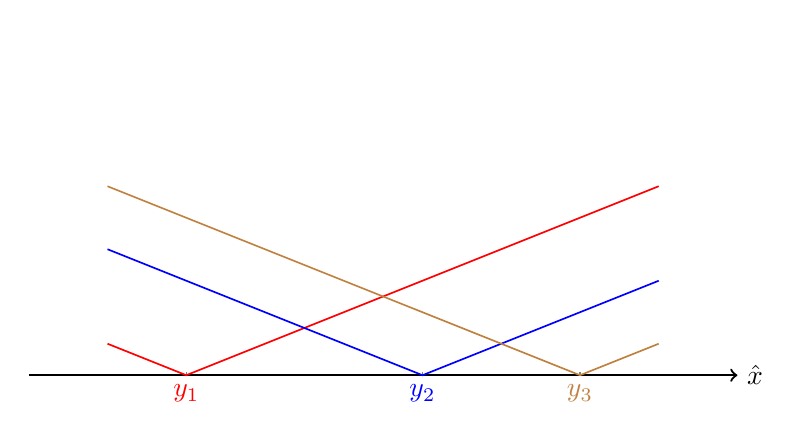
\begin{tikzpicture}[yscale=0.4]
      \draw[thick,->] (0,0)--(9,0);
      \node [anchor=west] at (9,0) {$\hat x$};
      \draw[thin,gray] (2,0)--(2,0.1);
      \draw[thin,gray] (5,0)--(5,0.1);
      \draw[thin,gray] (7,0)--(7,0.1);
      \draw[thick,white](1,11)--(2,8)--(5,5)--(7,7)--(8,10);
      \node [anchor=north] at (2,0) {\color{red}{$y_1$}};
      \draw[semithick,red](1,1)--(2,0)--(8,6);
      \node [anchor=north] at (5,0) {\color{blue}{$y_2$}};
      \draw[semithick,blue](1,4)--(5,0)--(8,3);
      \node [anchor=north] at (7,0) {\color{brown}{$y_3$}};
      \draw[semithick,brown](1,6)--(7,0)--(8,1);
    \end{tikzpicture}
  \end{figure}
  If we interpret the function $|y_i-\hat x|$ as a potential function generate by sensor $i$, then we can see that sensor $i$ is dragging $\hat x$ towards $y_i$ with $1$ unit of force. The equilibrium point will be at the middle $y_i$.
\end{frame}

\begin{frame}{Another Example}
  Suppose the following sensory model:
  \begin{align*}
    y = \begin{bmatrix}
      1\\
      1\\
      3
    \end{bmatrix}x + w+a ,\,\|a\|_0\leq 1.
  \end{align*}
  Then the following estimator is not resilient:
  \begin{align*}
    g(y) = \argmin_{\hat x}  |y_1-\hat x|+|y_2-\hat x|+|y_3-3\hat x|.
  \end{align*}
  In fact, we can rewrite it as
  \begin{align*}
    g(y) = \argmin_{\hat x}  |y_1-\hat x|+|y_2-\hat x|+3\left|\frac{y_3}{3}-\hat x\right| = \frac{y_3}{3}
  \end{align*}
  Sensor $3$ generates $3$ unit of force comparing to $1$ unit of force from sensor $1$ and $2$.
\end{frame}

\begin{frame}{Sufficient Condition For Resiliency}
  \begin{theorem}
    If the following conditions hold, then the estimation is resilient:
    \begin{enumerate}
      \item For all $i$, the following limit is well-defined:
	\begin{align*}
	  \lim_{t\rightarrow\infty}\frac{f_i(tH_iu)}{t} = C_i(u) < \infty.
	\end{align*}
      \item For any $u\neq 0$ and any index set $\mathcal I$ of cardinality $c$, the following inequality hold:
	\begin{align*}
	  \sum_{i\in \mathcal I} C_i(u) < \sum_{i\in \mathcal I^c} C_i(u). 
	\end{align*}
    \end{enumerate}
  \end{theorem}
  Roughly speaking $C_i(u)$ characterize how powerful a single sensor $i$ is along direction $u$. The condition can be interpreted as the no $c$ sensors combined can be more powerful than the remaining $m-c$ sensors.
\end{frame}

\begin{frame}{Necessary Condition For Resiliency}
  \begin{theorem}
    If the one of the following conditions is violated, then the estimation is not resilient:
    \begin{enumerate}
      \item There exists an $i$ and $u$, such that
	\begin{align*}
 \lim_{t\rightarrow\infty}\frac{f_i(tH_iu)}{t} = \infty.
	\end{align*}
      \item There exists a $u\neq 0$ and an index set $\mathcal I$ of cardinality $c$, such that
	\begin{align*}
	  \sum_{i\in \mathcal I} C_i(u) > \sum_{i\in \mathcal I^c} C_i(u). 
	\end{align*}
    \end{enumerate}
  \end{theorem}
  Notice that we only have a trivial gap for the case:
\begin{align*}
  \sum_{i\in \mathcal I} C_i(u) = \sum_{i\in \mathcal I^c} C_i(u).
\end{align*}	  
\end{frame}

\begin{frame}{In Summary\footcite{Han2019}}
  \begin{itemize}
    \item We design a convex optimization based estimator
  \begin{align*}
    \hat x = g(y) \triangleq \argmin_{\hat x} \sum_{i=1}^m f_i(y_i-H_i \hat x).
  \end{align*}
    \item Difficult to verify the resiliency condition
      \begin{align*}
	\sum_{i\in \mathcal I} C_i(u) < \sum_{i\in \mathcal I^c} C_i(u). 
      \end{align*}
    \item Easy to compute via convex optimization
    \item If $f_i$ is the Huber loss function, then we could recover the least square estimate if:
      \begin{itemize}
	\item there is no attack
	\item the noise is "small"
      \end{itemize}
  \end{itemize}
\end{frame}

\begin{frame}{Simulation IEEE 14-bus System}
  \begin{figure}[ht]
    \centering
    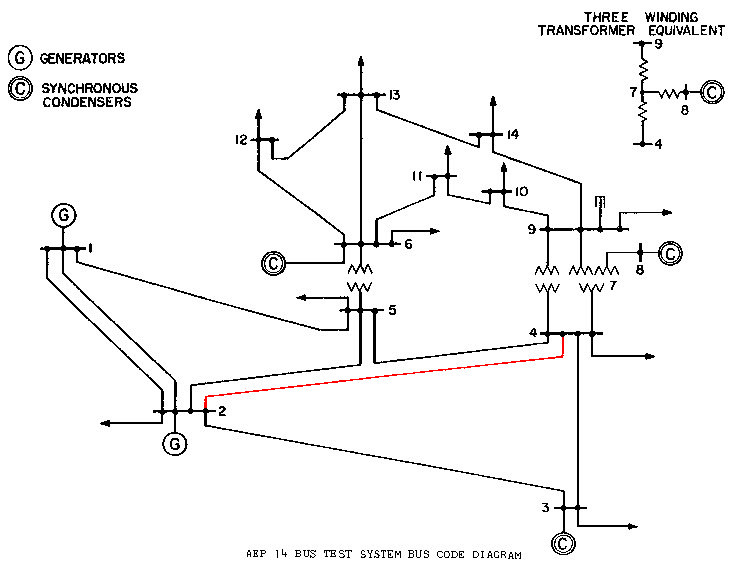
\includegraphics[width=0.60\textwidth]{ieee14.jpg}
  \end{figure}
  We assume $c=1$ and the flow sensor on the red line is being attacked.
\end{frame}

\begin{frame}{Simulation IEEE 14-bus System}
  \begin{figure}[ht]
    \begin{center}

      \setlength{\figureheight}{6cm}
      \setlength{\figurewidth}{10cm}
      \definecolor{mycolor1}{rgb}{1.00000,0.00000,1.00000}%
      % 
      \begin{tikzpicture}

	\begin{axis}[%
	  width=\figurewidth,
	  height=\figureheight,
	  at={(1.527in,1.083in)},
	  scale only axis,
	  xmin=0.95,
	  xmax=2.4,
	  xlabel={Normalized MSE of the estimators without attack},
	  xmajorgrids,
	  ymin=0.95,
	  ymax=2.5,
	  ylabel={Normalized MSE when under attack},
	  ymajorgrids,
	  axis background/.style={fill=white},
	  legend style={at={(0.597,0.528)},anchor=south west,legend cell align=left,align=left,draw=white!15!black}
	  ]
	  \addplot [color=blue,dashed,line width=1.5pt,mark=triangle,mark options={solid},forget plot]
	    table[row sep=crcr]{%
	      2.16434829886514	2.41673714136766\\
	      1.49824142620916	1.6273922047888\\
	      1.46836558726546	1.61304395019434\\
	      1.42878218405531	1.58080265845186\\
	      1.33509034059386	1.48317348510781\\
	      1.24979953097586	1.4011442907391\\
	      1.20190884155895	1.36475282176979\\
	      1.14816845697376	1.32743887772808\\
	      1.104692902235	1.30458587111275\\
	      1.0727554366346	1.2930587844785\\
	      1.04837293442887	1.29286647088633\\
	      1.03276380632143	1.30464750437787\\
	      1.02491383863213	1.32636243694814\\
	      1.0209295289153	1.35606289076979\\
	      1.01470702949196	1.40680155569416\\
	      1.00686189169388	1.48274325705327\\
	      1.00166658882151	1.69020329692052\\
	      1.00012894457222	2.29806950301701\\
	    };

	  \addplot [color=mycolor1,dashed,forget plot]
	    table[row sep=crcr]{%
	      1	1\\
	      2.2	1\\
	    };
	  \addplot [color=mycolor1,dashed,forget plot]
	    table[row sep=crcr]{%
	      1	1\\
	      1	2.5\\
	    };
	  \node[right, align=left, text=blue]
	  at (axis cs:2.164,2.417) {$\text{   }\leftarrow\text{ }\gamma\rightarrow 0$};
	  \node[right, align=left, text=blue]
	  at (axis cs:1.335,1.483) {$\text{   }\leftarrow\text{ }\gamma\text{=0.5}$};
	  \node[right, align=left, text=blue]
	  at (axis cs:1.202,1.365) {$\text{   }\leftarrow\text{ }\gamma\text{=1}$};
	  \node[right, align=left, text=blue]
	  at (axis cs:1.073,1.293) {$\text{   }\leftarrow\text{ }\gamma\text{=1.9}$};
	  \node[right, align=left, text=blue]
	  at (axis cs:1.02,1.356) {$\leftarrow\gamma\text{=3}$};
	  \node[right, align=left, text=blue]
	  at (axis cs:1,2.298) {$\text{   }\leftarrow\text{ }\gamma\text{=7}$};
	  \node[right, align=left, text=mycolor1]
	  at (axis cs:1,2.4) {$\text{   }\leftarrow\text{ LSE}$};
	  \node[right, align=left, text=mycolor1]
	  at (axis cs:1.9,1.14) {Oracle LSE};
	  \node[right, align=left, text=mycolor1]
	  at (axis cs:1.9,1.07) {$\text{     ~~~~~}\downarrow$};
	\end{axis}
      \end{tikzpicture}%
    \end{center}
  \end{figure}
\end{frame}

\subsection{Dynamic State Estimation}
\begin{frame}{Dynamic State Estimation}
  \begin{enumerate}
    \item Consider the following dynamic system
      \begin{align}
	x(k+1) = A x(k) + w(k),\, y(k) = C x(k) + v(k) + a(k).
      \end{align}
    \item A linear fixed-gain estimator:
      \begin{align}
	\hat x(k+1) = A \hat x(k) + K(y(k+1)-CA\hat x(k)),
      \end{align}
      where $K$ is the estimation gain, and $A-KCA$ is stable.
      \begin{center}
	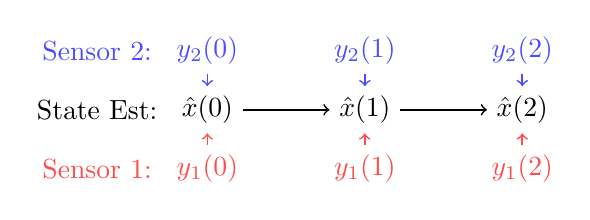
\begin{tikzpicture}[x=2cm, y=0.75cm]
	  \node at (-0.7,0) {State Est:};
	  \node [blue!70] at (-0.7,1) {Sensor 2:};
	  \node [red!70] at (-0.7,-1) {Sensor 1:};

	  \node            (x0)  at (0,0) {$\hat x(0)$};
	  \node [blue!70] (y20)  at (0,1)    {$y_2(0)$};
	  \node [red!70]  (y10)  at (0,-1)   {$y_1(0)$};
	  \draw [->,semithick,blue!70] (y20) to (x0);
	  \draw [->,semithick,red!70]  (y10) to (x0);

	  \node            (x1)  at (1,0) {$\hat x(1)$};
	  \node [blue!70] (y21)  at (1,1)    {$y_2(1)$};
	  \node [red!70]  (y11)  at (1,-1)   {$y_1(1)$};
	  \draw [->,semithick,blue!70] (y21) to (x1);
	  \draw [->,semithick,red!70]  (y11) to (x1);

	  \node            (x2)  at (2,0) {$\hat x(2)$};
	  \node [blue!70] (y22)  at (2,1)    {$y_2(2)$};
	  \node [red!70]  (y12)  at (2,-1)   {$y_1(2)$};
	  \draw [->,semithick,blue!70] (y22) to (x2);
	  \draw [->,semithick,red!70]  (y12) to (x2);

	  \draw [->,semithick] (x0) to (x1);
	  \draw [->,semithick] (x1) to (x2);
	\end{tikzpicture}
      \end{center}
    \item Captures most of the estimators: steady-state Kalman filter, $H_2$/$H_\infty$ estimator
    \item The error introduced by the attack may accumulate over time.
  \end{enumerate}
\end{frame}

\begin{frame}{Fundamental Limit}
  If the system becomes undetectable after removing $2c$ sensors, then there exists an attack on $c$ sensors, such that NO estimator can have bounded estimation error \footcite{Nakahira2018}.
\end{frame}

\begin{frame}{Dynamic State Estimate: A Moving Horizon Approach}
In order to convert the dynamic estimation problem into a static one, we can use a moving horizon approach\footcite{Fawzi2014}\footcite{Shoukry2017}:
  \begin{center}
    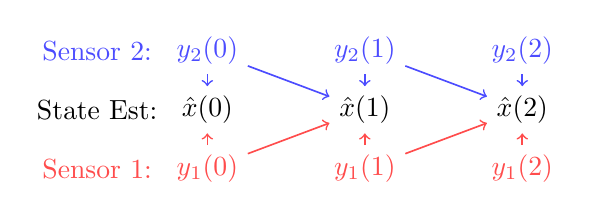
\begin{tikzpicture}[x=2cm, y=0.75cm]
      \node at (-0.7,0) {State Est:};
      \node [blue!70] at (-0.7,1) {Sensor 2:};
      \node [red!70] at (-0.7,-1) {Sensor 1:};

      \node            (x0)  at (0,0) {$\hat x(0)$};
      \node [blue!70] (y20)  at (0,1)    {$y_2(0)$};
      \node [red!70]  (y10)  at (0,-1)   {$y_1(0)$};
      \draw [->,semithick,blue!70] (y20) to (x0);
      \draw [->,semithick,red!70]  (y10) to (x0);

      \node            (x1)  at (1,0) {$\hat x(1)$};
      \node [blue!70] (y21)  at (1,1)    {$y_2(1)$};
      \node [red!70]  (y11)  at (1,-1)   {$y_1(1)$};
      \draw [->,semithick,blue!70] (y21) to (x1);
      \draw [->,semithick,red!70]  (y11) to (x1);
      \draw [->,semithick,blue!70] (y20) to (x1);
      \draw [->,semithick,red!70]  (y10) to (x1);

      \node            (x2)  at (2,0) {$\hat x(2)$};
      \node [blue!70] (y22)  at (2,1)    {$y_2(2)$};
      \node [red!70]  (y12)  at (2,-1)   {$y_1(2)$};
      \draw [->,semithick,blue!70] (y22) to (x2);
      \draw [->,semithick,red!70]  (y12) to (x2);
      \draw [->,semithick,blue!70] (y21) to (x2);
      \draw [->,semithick,red!70]  (y11) to (x2);
    \end{tikzpicture}
  \end{center}

  However, the historical data are discarded and the estimation performance may be poor when the system is operating normally.
\end{frame}

\begin{frame}{Dynamic State Estimate: A Local Estimator Approach}
  We propose to store historical data in the local estimations:
  \begin{center}
    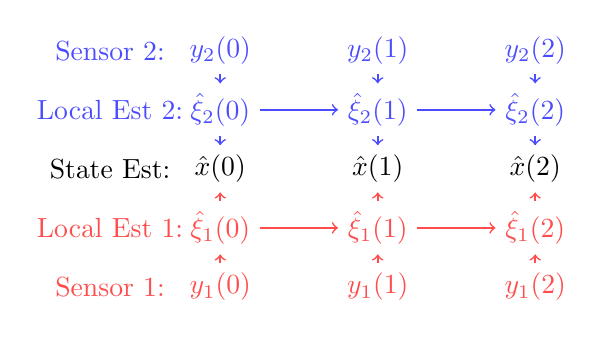
\begin{tikzpicture}[x=2cm, y=0.75cm]
      \node at (-0.7,0) {State Est:};
      \node [blue!70] at (-0.7,2) {Sensor 2:};
      \node [blue!70] at (-0.7,1) {Local Est 2:};
      \node [red!70] at (-0.7,-2) {Sensor 1:};
      \node [red!70] at (-0.7,-1) {Local Est 1:};

      \node            (x0)  at (0,0)    {$\hat x(0)$};
      \node [blue!70] (y20)  at (0,2)       {$y_2(0)$};
      \node [blue!70] (x20)  at (0,1)  {$\hat \xi_2(0)$};
      \node [red!70]  (y10)  at (0,-2)      {$y_1(0)$};
      \node [red!70]  (x10)  at (0,-1) {$\hat \xi_1(0)$};
      \draw [->,semithick,blue!70] (y20) to (x20);
      \draw [->,semithick,red!70]  (y10) to (x10);
      \draw [->,semithick,blue!70] (x20) to  (x0);
      \draw [->,semithick,red!70]  (x10) to  (x0);

      \node            (x1)  at (1,0)    {$\hat x(1)$};
      \node [blue!70] (y21)  at (1,2)       {$y_2(1)$};
      \node [blue!70] (x21)  at (1,1)  {$\hat \xi_2(1)$};
      \node [red!70]  (y11)  at (1,-2)      {$y_1(1)$};
      \node [red!70]  (x11)  at (1,-1) {$\hat \xi_1(1)$};
      \draw [->,semithick,blue!70] (y21) to (x21);
      \draw [->,semithick,red!70]  (y11) to (x11);
      \draw [->,semithick,blue!70] (x21) to  (x1);
      \draw [->,semithick,red!70]  (x11) to  (x1);

      \node            (x2)  at (2,0)    {$\hat x(2)$};
      \node [blue!70] (y22)  at (2,2)       {$y_2(2)$};
      \node [blue!70] (x22)  at (2,1)  {$\hat \xi_2(2)$};
      \node [red!70]  (y12)  at (2,-2)      {$y_1(2)$};
      \node [red!70]  (x12)  at (2,-1) {$\hat \xi_1(2)$};
      \draw [->,semithick,blue!70] (y22) to (x22);
      \draw [->,semithick,red!70]  (y12) to (x12);
      \draw [->,semithick,blue!70] (x22) to  (x2);
      \draw [->,semithick,red!70]  (x12) to  (x2);

      \draw [->,semithick,blue!70] (x20) to (x21);
      \draw [->,semithick,blue!70] (x21) to (x22);
      \draw [->,semithick,red!70] (x10) to (x11);
      \draw [->,semithick,red!70] (x11) to (x12);
    \end{tikzpicture}
  \end{center}
  \begin{enumerate}
    \item Construct local estimators for each sensor (which uses only the local measurements)
    \item Reconstruct the global estimator 
  \end{enumerate}
\end{frame}

%\begin{frame}{Local Estimator Design}
%  \begin{enumerate}
%    \item  Choose $L_i$ such that $A-L_iCA$ shares the same eigenvalues as $A-KCA$ (requires observability)
%      \begin{align*}
%	\hat x_i(k) = A \hat x_i(k) + L_i (y_i(k)-CA\hat x_i(k)).
%      \end{align*}  
%    \item The global estimate can be recovered as
%      \begin{align*}
%	\hat x(k) = F_1\hat x_1(k)+\dots+F_m\hat x_m(k).
%      \end{align*}
%    \item More importantly, it can be written as the solution of a quadratic programming problem:
%      \begin{align*}
%      &\mathop{\textrm{minimize}}\limits_{\hat x(k),\hat e(k)}&
%      & \frac{1}{2}\hat e(k)^T \tilde W^{-1} \hat e(k)\\
%      &\textrm{subject to} &
%      &\hat x_i(k)  =  \hat x(k) + \hat e_i(k),&
%      \end{align*}
%  \end{enumerate}
%\end{frame}

\begin{frame}{Local Estimator Design}
  We make the following assumptions:
  \begin{enumerate}
    \item The system $(A,C)$ is observable. However the whole state space may not be observable for individual sensors.  
    \item The eigenvalues of $A-KCA$ are distinct.   
    \item $A-KCA$ do not share eigenvalues with $A$.
  \end{enumerate}
  As a result, we could design the estimator as:
  \begin{align*}
    \hat \xi_i(k) = \Lambda \hat \xi_i(k) + \mathbf 1 y_i(k+1), 
  \end{align*}  
  where
  \begin{enumerate}
    \item $\Lambda = diag (\lambda_1, \ldots, \lambda_n)$ is a diagonal matrix, such that $A-KCA = V\Lambda V^{-1}.$
      \item $\mathbf 1$ is an all-one vector of dimension $n$.
  \end{enumerate}
\end{frame}

\begin{frame}{Properties of the Local Estimator in the Absence of Attack}
  \begin{enumerate}
    \item $\hat \xi_i$ is a stable estimate of $G_ix$, where
      \begin{align*}
	G_{i} \triangleq
	\begin{bmatrix}
	  C_{i} A\left(A-\lambda_{1} I\right)^{-1} \\
	  \vdots \\
	  C_{i} A\left(A-\lambda_{n} I\right)^{-1}
	\end{bmatrix}.
      \end{align*}
    \item The null space of $G_i$ matrix is exactly the unobservable state space for sensor $i$.
    \item  The estimation error $\epsilon_i(k)\triangleq G_i x(k)-\xi_i(k)$ follows:
      \begin{align*}
	\epsilon_{i}(k+1)= \Lambda \epsilon_{i}(k)+\left(G_{i}-\mathbf{1} C_{i}\right) w(k) -\mathbf{1} v_{i}(k+1).
      \end{align*}
    \item The Kalman estimate can be recovered as the solution of a least square problem:
      \begin{align*}
      &\mathop{\textrm{minimize}}\limits_{\hat x(k),\hat \epsilon(k)}&
      & \frac{1}{2}\hat \epsilon(k)^T \tilde W^{-1} \hat \epsilon(k)\\
      &\textrm{subject to} &
      &\hat \xi_i(k)  =  G_i\hat x(k) + \hat \epsilon_i(k),&
      \end{align*}
      where the matrix $\tilde W$ is the asymptotic covariance of $[\epsilon_1^T,\ldots ,\epsilon_n^T]$.
  \end{enumerate}
\end{frame}

\begin{frame}{Securing the Global Estimate with LASSO}
  \begin{itemize}
    \item  In the presence of attack, the estimation error follows:
      \begin{align*}
	\epsilon_{i}(k+1)= \Lambda \epsilon_{i}(k)+\left(G_{i}-\mathbf{1} C_{i}\right) w(k) -\mathbf{1} v_{i}(k+1) - \mathbf{1} a_{i}(k+1) .
      \end{align*}
    \item We can secure the global estimator using LASSO:
      \begin{align*}
    &\mathop{\textrm{minimize}}\limits_{\hat x(k),\hat \epsilon(k), \hat \nu(k)}&
    & \frac{1}{2}\hat \epsilon(k)^T \tilde W^{-1} \hat \epsilon(k) + \gamma \sum_{i=1}^m \|\hat \nu_i(k)\|_1\\
    &\textrm{subject to} &
    &\hat \xi_i(k)  =  G_i\hat x(k) + \hat \epsilon_i(k)+\hat \nu_i(k).&
      \end{align*}
  \end{itemize}
\end{frame}

\begin{frame}{Efficiency and Security\footcite{Liu2017}}
  \begin{block}{Efficiency}
    \begin{itemize}
      \item In the absence of attack, we recover the Kalman estimate if the noise is "small".
      \item Given a probability $p<1$, we can tune $\gamma$ such that we recover KF with probability $p$.
    \end{itemize}
  \end{block}
  \begin{block}{Security}
    In the presence of attack, the estimator is stable if for any $u\neq 0$ and any index set $\mathcal I$ of cardinality $c$, the following inequality hold:
    \begin{align*}
      \sum_{i\in \mathcal I} \|G_iu\|_1 < \sum_{i\in \mathcal I^c} \|G_iu\|_1. 
    \end{align*}
  \end{block}
\end{frame}

\begin{frame}{The Last Piece of the Puzzle\footcite{Mao2019}}
  \begin{itemize}
    \item Consider a $2$-dimensional system with $A = diag(1,2)$ 
    \item The observable space for a sensor can only be $\{x_1\},\,\{x_2\}$ or $\{x_1,\,x_2\}$
    \item It is not possible for the observable space to be $\{ax_1+bx_2\}$ with non-zero $a,b$!
    \item As such, we could always transform $G_i$ into
      \begin{align*}
	G_i = \begin{bmatrix}
	  1&0\\
	  0&0
	  \end{bmatrix} ,\,\begin{bmatrix}
	  0&1\\
	  0&0
	  \end{bmatrix} ,\,or\,\begin{bmatrix}
	  1&0\\
	  0&1
	\end{bmatrix} .
      \end{align*}
  \end{itemize}
\end{frame}

\begin{frame}{In Summary}
  Given a probability $p<1$, if all unstable eigenvalues of the system matrix $A$ has geometric multiplicity of $1$, then we can design an estimator, such that
  \begin{enumerate}
    \item Close to optimal {\bf efficiency}: In the absence of attack, the estimator coincides with the optimal Kalman estimator with probability $p$.
    \item Optimal {\bf security}: The estimator is resilient against $c$ malicious sensors, assuming that every unstable state can be observed by at least $2c+1$ sensors.
  \end{enumerate}
  It is easy to certify the security of the estimator and compute the state estimate in real time. 
\end{frame}

\begin{frame}{Numerical Example: Inverted pendulum}
  \centering
  \begin{columns}
    \begin{column}{0.5\textwidth}
      \scalebox{0.7}{


%\tikzsetnextfilename{PIDBode}
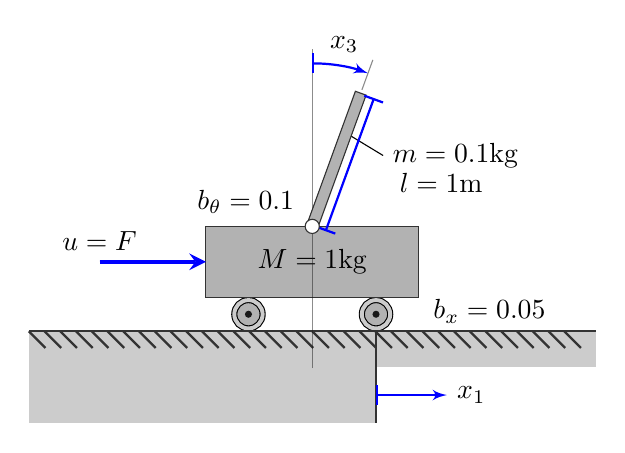
\begin{tikzpicture}[> = latex',%
	scale = 0.9]
	\tikzset{%
		interface/.style={
			% The border decoration is a path replacing decorator. 
			% For the interface style we want to draw the original path.
			% The postaction option is therefore used to ensure that the
			% border decoration is drawn *after* the original path.
			postaction={draw, decorate, decoration={border, angle=-45,
					amplitude=0.3cm, segment length=2mm}}},
		helparrow/.style={>=latex', blue, thick},
		% helparrow/.style={>=latex', draw=blue, fill=blue, very thick},
		helpline/.style={thin, black!90, opacity=0.5},
		force/.style={>=stealth, draw=blue, fill=blue, ultra thick},
	}
	\def\ground{%
		\fill [black!20] (0, 0) rectangle (49mm, -13mm);
		\fill [black!20] (49mm, 0) rectangle (80mm, -5mm);
		\draw [thick, black!80, interface] (0, 0) -- (80mm, 0);
		\draw [thick, black!80] (49mm, 0) -- +(0, -13mm);
		\draw [|->, helparrow] (49mm, -9mm) -- ++(10mm, 0) node [right] {\color{black} $x_1$ };
	}
	
	\def\cart{
		\filldraw [%thick,%
		draw = black!80,%
		fill = black!40,%
		top color = black!30,%
		bottom color = black!30,%
		% pattern=horizontal lines gray,%
		] (0,0) rectangle (30mm, 10mm);
		\node at (15mm, 5mm) {$M=1$kg};
		\draw[->, force] (-15mm, 5mm) node [above] {$u=\ensuremath{\vv{F}}$} -- (0, 5mm);
		\node at (40mm, -2mm) {$b_x = 0.05$};
	}
	
	\def\pendulum{%
		\filldraw [%thick,%
		draw = black!80,%
		% fill = black!25,%
		left color=black!30,%
		bottom color=black!30,%
		% pattern=horizontal lines gray,%
		] (-0.8mm, 0) rectangle (0.8mm, 20mm);
		\draw [|-|, helparrow] (2mm, 0mm) -- ++(0mm, 20mm);
		\node at (15mm, 12mm) {$l=1$m};
		\node at (-10mm, 0mm) {$b_\theta=0.1$}; 
	}
	
	\def\joint{%
		\filldraw [%thick,%
		draw = black!80,%
		fill = white,%
		% pattern=horizontal lines gray,%
		] (0, 0) circle (1mm);
	}
	
	\def\wheel{%
%		\fill [thin,%
%		fill = black!70,%	path fading = south
%	] (0, 0) circle (1.75mm);
%		\begin{scope}
%			\clip (0, 0) circle (1.75mm);
%			\fill [fill=black!30,] (0, -1mm) circle (2mm);
%		\end{scope}
		\fill [fill=black!30,] (0, 0mm) circle (2mm);
		\fill [fill=black!90] (0, 0) circle (0.5mm);
		\draw [thin,%
		double = black!20,%
		double distance = 0.5mm] (0, 0) circle (2mm);
	}

	\begin{scope}
		\wheel
	\end{scope}
	\begin{scope}[xshift=18mm]
		\wheel
	\end{scope}
	\begin{scope}[xshift=-31mm, yshift=-2.4mm]
		\ground
	\end{scope}
	\begin{scope}[shift = {(-6mm, 2.4mm)}]
		\cart
	\end{scope}
	\begin{scope}[shift = {(9mm, 12.4mm)}]
		\draw [helpline] (0, -20mm) -- (0, 25mm);
		\draw [helpline] (70:20.5mm) -- (70:25mm);
		\draw [|->, helparrow] (0, 23mm) 
		arc [radius=23mm, start angle=90, delta angle=-20] ;
		\node at (80:26mm) {$x_3$};
%		\draw [|->, helparrow] (0, -9mm) 
%		arc [radius=9mm, start angle=-90, delta angle=195] ;
%		\node [above right] at (50:8.5mm) {$\theta$};
		\draw [thin] (70:14mm) -- (10mm, 10mm) 
		node [right] {$m=0.1$kg};
	\end{scope}
	\begin{scope}[shift = {(9mm, 12.4mm)}, rotate=-20]
		\pendulum
	\end{scope}
	\begin{scope}[shift = {(9mm, 12.4mm)}]
		\joint
	\end{scope}
\end{tikzpicture}


%\begin{tikzpicture}[> = latex',%
%	scale = 1,%
%	text = blue]
%	\begin{scope}
%		\wheel
%	\end{scope}
%	\begin{scope}[xshift=18mm]
%		\wheel
%	\end{scope}
%	\begin{scope}[xshift=-31mm, yshift=-2.4mm]
%		\ground
%	\end{scope}
%	\begin{scope}[shift = {(-6mm, 2.4mm)}]
%		\cart
%	\end{scope}
%	\begin{scope}[shift = {(9mm, 12.4mm)}]
%		\draw [helpline] (0, -20mm) -- (0, 25mm);
%		\draw [helpline] (110:20.5mm) -- (110:25mm);
%		\draw [|->, helparrow] (0, 23mm) 
%		arc [radius=23mm, start angle=90, delta angle=20] ;
%		\node at (97:25mm) {$\theta'$};
%		\draw [|->, helparrow] (0, -9mm) 
%		arc [radius=9mm, start angle=-90, delta angle=195] ;
%		\node [above right] at (50:8.5mm) {$\theta$};
%		\draw [thin] (110:14mm) -- (-10mm, 10mm) 
%		node [left] {$m$, $I$};
%	\end{scope}
%	\begin{scope}[shift = {(9mm, 12.4mm)}, rotate=20]
%		\pendulum
%	\end{scope}
%	\begin{scope}[shift = {(9mm, 12.4mm)}]
%		\joint
%	\end{scope}
%\end{tikzpicture}}
    \end{column}
    \begin{column}{0.5\textwidth}
      $x_1$: cart position

      $x_2$: cart velocity

      $x_3$: pendulum angle

      $x_4$: pendulum angle velocity

      Linearize at $x_3=x_4=0$, 

      Sample with interval $T_s=0.02$.
    \end{column}
  \end{columns}

  \vspace{-1pt}
  {\footnotesize
    \begin{align*}
      x(k+1)=\begin{bmatrix}
	1  \hspace{-2pt}&\hspace{-2pt}   2.0\hspace{-2pt}\cdot\hspace{-2pt} 10^{-2}  \hspace{-2pt}&\hspace{-2pt}  -2.0\hspace{-2pt}\cdot\hspace{-2pt} 10^{-4}  \hspace{-2pt}&\hspace{-2pt}  1.9\hspace{-2pt}\cdot\hspace{-2pt} 10^{-5}\\
	0  \hspace{-2pt}&\hspace{-2pt}   1.0\hspace{-2pt}\cdot\hspace{-2pt} 10^{0}   \hspace{-2pt}&\hspace{-2pt} -2.0\hspace{-2pt}\cdot\hspace{-2pt} 10^{-2}  \hspace{-2pt}&\hspace{-2pt}   1.8\hspace{-2pt}\cdot\hspace{-2pt} 10^{-3}\\
	0  \hspace{-2pt}&\hspace{-2pt}   1.0\hspace{-2pt}\cdot\hspace{-2pt} 10^{-5} \hspace{-2pt}&\hspace{-2pt}   1.0\hspace{-2pt}\cdot\hspace{-2pt} 10^{0} \hspace{-2pt}&\hspace{-2pt}   2.0\hspace{-2pt}\cdot\hspace{-2pt} 10^{-2}\\
	0  \hspace{-2pt}&\hspace{-2pt}   1.0\hspace{-2pt}\cdot\hspace{-2pt} 10^{-3}\hspace{-2pt}&\hspace{-2pt}  2.1\hspace{-2pt}\cdot\hspace{-2pt} 10^{-1}  \hspace{-2pt}&\hspace{-2pt}  9.8\hspace{-2pt}\cdot\hspace{-2pt} 10^{-1}
	\end{bmatrix}x(k)+\begin{bmatrix}
	2.0\hspace{-2pt}\cdot\hspace{-2pt} 10^{-4}\\
	2.0\hspace{-2pt}\cdot\hspace{-2pt} 10^{-2}\\
	-2.0\hspace{-2pt}\cdot\hspace{-2pt} 10^{-4}\\
	-2.0\hspace{-2pt}\cdot\hspace{-2pt} 10^{-2}
      \end{bmatrix}
      u(k)+w(k).
    \end{align*}
    \begin{align*}
      y(k)=
      \begin{bmatrix}
	1\hspace{-2pt}&\hspace{-2pt} 0 \hspace{-2pt}&\hspace{-2pt}0 \hspace{-2pt}&\hspace{-2pt}0\\
	1\hspace{-2pt}&\hspace{-2pt} 0 \hspace{-2pt}&\hspace{-2pt}0 \hspace{-2pt}&\hspace{-2pt}0\\
	1\hspace{-2pt}&\hspace{-2pt} 0 \hspace{-2pt}&\hspace{-2pt}0 \hspace{-2pt}&\hspace{-2pt}0\\
	0\hspace{-2pt}&\hspace{-2pt} 0 \hspace{-2pt}&\hspace{-2pt}1 \hspace{-2pt}&\hspace{-2pt}0
      \end{bmatrix}x(k)+v(k)+a(k).
  \end{align*} }
\end{frame}
\begin{frame}{Performance without attack}
  \begin{figure}[htpb!]
    \centering
    \scalebox{0.65}{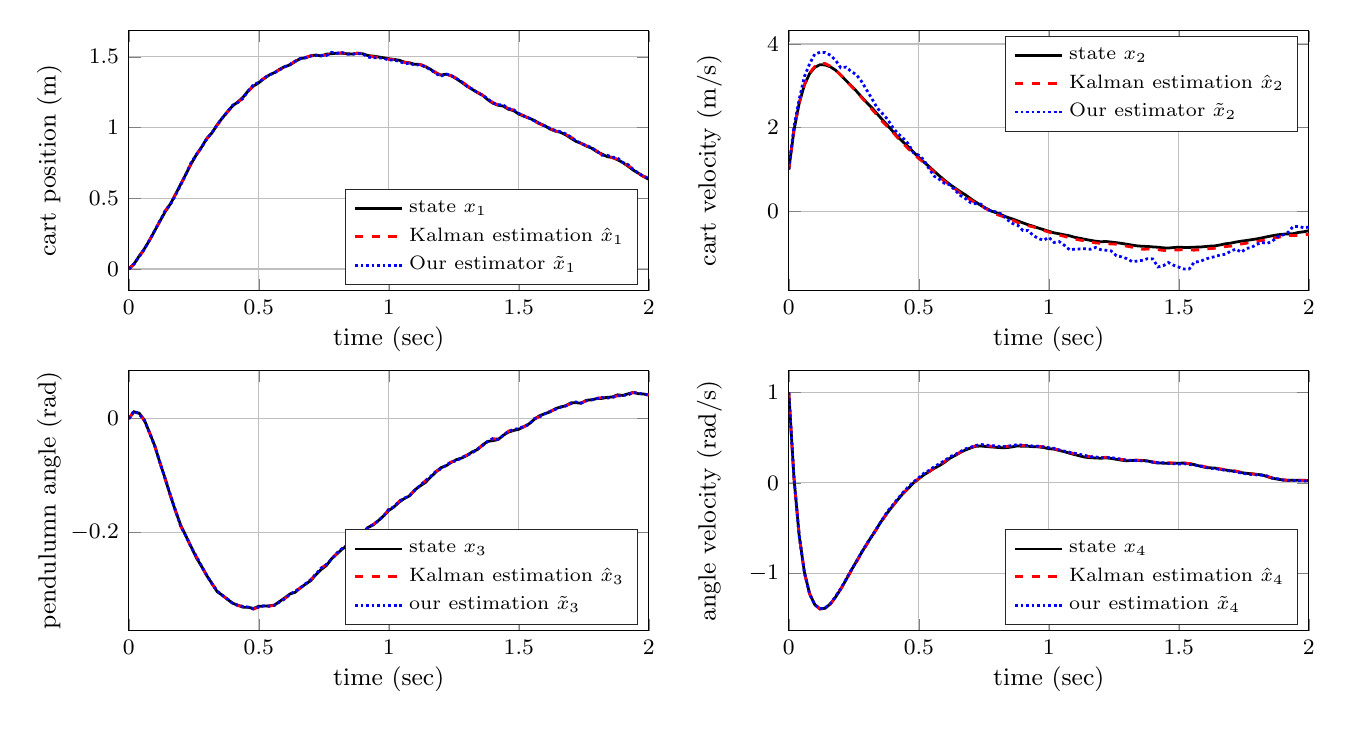
\begin{tikzpicture}
\begin{axis}
[	width=2.6in,
	height=1.3in,
	at={(0in,1.7in)},
	scale only axis,
	xmin=0,
	xmax=2.0,
	xlabel={\small time (sec)},
	ylabel={\small cart position (m)},
	x label style={at={(axis description cs:0.5,-0.1)},anchor=north},
	y label style={at={(axis description cs:-0.11,.5)},anchor=south},
	xticklabel style = {font=\footnotesize},
	yticklabel style = {font=\footnotesize},
	axis background/.style={fill=white},
	xmajorgrids,
	ymajorgrids,
	legend style={at={(0.98,0.02)}, anchor=south east, legend cell align=left, align=left, draw=white!15!black, font=\scriptsize }]
	 \addplot [color={black}, line width=1pt]
	table[row sep={\\}]
	{
 0.0  0.0  \\
0.02  0.03513048308256195  \\
0.04  0.0914419059773598  \\
0.06  0.1427778787943515  \\
0.08  0.20340397252067047  \\
0.1  0.27125016952880654  \\
0.12  0.33866874289613796  \\
0.14  0.40444843392896823  \\
0.16  0.46015949841787734  \\
0.18  0.5289069560917001  \\
0.2  0.6012564469268484  \\
0.22  0.671516604288933  \\
0.24  0.7439326698612437  \\
0.26  0.8082019623524164  \\
0.28  0.8613988630585795  \\
0.3  0.9229014124726718  \\
0.32  0.9627944492478866  \\
0.34  1.0198488236259264  \\
0.36  1.0678031171226763  \\
0.38  1.1139131874770454  \\
0.4  1.1540061381552729  \\
0.42  1.1817601868900285  \\
0.44  1.2153756793882182  \\
0.46  1.2610010644181515  \\
0.48  1.293667654117393  \\
0.5  1.3165928728936251  \\
0.52  1.3456607164297567  \\
0.54  1.3711705993370278  \\
0.56  1.3880813521098108  \\
0.58  1.4119643858187543  \\
0.6  1.4306314658383006  \\
0.62  1.4425883212114448  \\
0.64  1.4662379310448435  \\
0.66  1.4886979846322503  \\
0.68  1.4923086118898035  \\
0.7  1.5069041141339614  \\
0.72  1.5128680594921478  \\
0.74  1.505743231730095  \\
0.76  1.5189247374151202  \\
0.78  1.5218381993746002  \\
0.8  1.5255446307745213  \\
0.82  1.5253720117652096  \\
0.84  1.5217505378866258  \\
0.86  1.519753386225738  \\
0.88  1.5257526690458258  \\
0.9  1.521386537923482  \\
0.92  1.5089559694196168  \\
0.94  1.5049195077352266  \\
0.96  1.4993578292639884  \\
0.98  1.493191880058802  \\
1.0  1.4864024420058506  \\
1.02  1.4818259580594746  \\
1.04  1.475808315831528  \\
1.06  1.462990519709879  \\
1.08  1.4570631794200655  \\
1.1  1.4471759284474504  \\
1.12  1.446272982684707  \\
1.14  1.4313922548235627  \\
1.16  1.4124330091086377  \\
1.18  1.3872010233567227  \\
1.2  1.3711358431710576  \\
1.22  1.3771278026366942  \\
1.24  1.3667791681890535  \\
1.26  1.3445038037339296  \\
1.28  1.3202679649240783  \\
1.3  1.2930882108314934  \\
1.32  1.2708701152599298  \\
1.34  1.248239872310746  \\
1.36  1.2293771367777346  \\
1.38  1.1977995399651467  \\
1.4  1.172303904975972  \\
1.42  1.1579161820351642  \\
1.44  1.1518067463014627  \\
1.46  1.12924061744534  \\
1.48  1.1195894705658813  \\
1.5  1.0955432603592228  \\
1.52  1.0797265742904583  \\
1.54  1.066608150282723  \\
1.56  1.0502266993513543  \\
1.58  1.0281772752372773  \\
1.6  1.0130822665150812  \\
1.62  0.9895403519101377  \\
1.64  0.9750991121836318  \\
1.66  0.9665183092659061  \\
1.68  0.9491107003879848  \\
1.7  0.9250252075044484  \\
1.72  0.9023279997906815  \\
1.74  0.8883577172905913  \\
1.76  0.868997041684394  \\
1.78  0.8542728121099745  \\
1.8  0.8295422463647049  \\
1.82  0.812162366888937  \\
1.84  0.7943357438050268  \\
1.86  0.7883783454959857  \\
1.88  0.7721739750301243  \\
1.9  0.7527806629178648  \\
1.92  0.7271547015768657  \\
1.94  0.699425481543776  \\
1.96  0.6770173029804786  \\
1.98  0.6539652107821747  \\
2.0  0.6339162103868775  \\
	}
	;\addlegendentry{state $x_1$}
	
	\addplot [color={red},dashed, line width=1pt]
	table[row sep={\\}]
	{
 0.0  0.0  \\
0.02  0.03459224381061867  \\
0.04  0.08529450384877155  \\
0.06  0.14037092177605182  \\
0.08  0.20553954051240308  \\
0.1  0.27194944336447746  \\
0.12  0.3421140054880376  \\
0.14  0.41203750940323125  \\
0.16  0.4622193750988459  \\
0.18  0.5275770920396385  \\
0.2  0.5965866800336724  \\
0.22  0.6697110178836443  \\
0.24  0.7482230113686512  \\
0.26  0.8092656626309191  \\
0.28  0.8603169832513828  \\
0.3  0.9190552078813129  \\
0.32  0.9650153184004646  \\
0.34  1.017537438416803  \\
0.36  1.0652639550276204  \\
0.38  1.110203819001036  \\
0.4  1.1547227063481849  \\
0.42  1.1795489385299753  \\
0.44  1.2081962408148317  \\
0.46  1.2550663978277128  \\
0.48  1.29773491819716  \\
0.5  1.3202634853421826  \\
0.52  1.3485493090138312  \\
0.54  1.3730537082664092  \\
0.56  1.3887333644343987  \\
0.58  1.4096399363306875  \\
0.6  1.4291719543335981  \\
0.62  1.4458626407157713  \\
0.64  1.4681322460180737  \\
0.66  1.4857860140746912  \\
0.68  1.4965623645092951  \\
0.7  1.5064593300461164  \\
0.72  1.5105362942780847  \\
0.74  1.5102375963545158  \\
0.76  1.510715778888172  \\
0.78  1.5270954377963672  \\
0.8  1.5246804945886832  \\
0.82  1.5285375327524982  \\
0.84  1.5219032482401056  \\
0.86  1.520849497046739  \\
0.88  1.5251716736489362  \\
0.9  1.524289721395395  \\
0.92  1.505448635516613  \\
0.94  1.4999695126483625  \\
0.96  1.4960501263894108  \\
0.98  1.4934718949769015  \\
1.0  1.4818326310727334  \\
1.02  1.480707330754286  \\
1.04  1.4726414641854848  \\
1.06  1.4602017028591072  \\
1.08  1.4578204430879882  \\
1.1  1.4469453164906172  \\
1.12  1.4458062938261007  \\
1.14  1.4329313953696996  \\
1.16  1.4160364457991061  \\
1.18  1.3897188031328918  \\
1.2  1.3679973969686312  \\
1.22  1.3751905872313022  \\
1.24  1.3655727389377705  \\
1.26  1.3488207107801553  \\
1.28  1.3275020222766156  \\
1.3  1.297676742947427  \\
1.32  1.2702012536827056  \\
1.34  1.2502056805120871  \\
1.36  1.2294028774129964  \\
1.38  1.2047001213441297  \\
1.4  1.1764390180689184  \\
1.42  1.16036795764531  \\
1.44  1.155022054177548  \\
1.46  1.133504665669269  \\
1.48  1.123504538352717  \\
1.5  1.1008427846179605  \\
1.52  1.0822931182727697  \\
1.54  1.0645682653691237  \\
1.56  1.0440920436330998  \\
1.58  1.0263246901040088  \\
1.6  1.0083507822846796  \\
1.62  0.9920679329287192  \\
1.64  0.976622670428748  \\
1.66  0.965578948875552  \\
1.68  0.9523055143949263  \\
1.7  0.9325703449798766  \\
1.72  0.907991669348745  \\
1.74  0.8873053457649742  \\
1.76  0.8709858398455673  \\
1.78  0.8557650883330062  \\
1.8  0.8339912648523344  \\
1.82  0.8066085662950583  \\
1.84  0.7985872884191355  \\
1.86  0.7867861486514177  \\
1.88  0.7761000737630973  \\
1.9  0.7490347746578546  \\
1.92  0.732851128940592  \\
1.94  0.703824889092848  \\
1.96  0.6780744090491957  \\
1.98  0.6534946070984852  \\
2.0  0.6408473560775105  \\
	}
	;\addlegendentry{{ Kalman estimation $\hat{x}_1$}}
    \addplot[densely dotted, color={blue}, line width=1pt]
        table[row sep={\\}]
        {
    0.0  1.4977176879243853e-7  \\
   0.02  0.035853490924953726  \\
   0.04  0.08728505927307653  \\
   0.06  0.1402910759956027  \\
   0.08  0.20552535131997382  \\
   0.1  0.2714941202711113  \\
   0.12  0.34142780537522516  \\
   0.14  0.41073226781224864  \\
   0.16  0.4544716293659916  \\
   0.18  0.523689684730239  \\
   0.2  0.59571397823773  \\
   0.22  0.6714956021666036  \\
   0.24  0.7527759703720808  \\
   0.26  0.8099977345031584  \\
   0.28  0.8585085304808415  \\
   0.3  0.9201763916641157  \\
   0.32  0.9634570022906116  \\
   0.34  1.0194972876060886  \\
   0.36  1.0682564396376053  \\
   0.38  1.1136126645917057  \\
   0.4  1.158888312085378  \\
   0.42  1.178120027939495  \\
   0.44  1.2073589678987888  \\
   0.46  1.26043900840599  \\
   0.48  1.3032407211239458  \\
   0.5  1.3196645821997441  \\
   0.52  1.3483934150336057  \\
   0.54  1.372515904226193  \\
   0.56  1.3860504677892873  \\
   0.58  1.4085218217648232  \\
   0.6  1.4289739159288626  \\
   0.62  1.4463131599581733  \\
   0.64  1.469263537104824  \\
   0.66  1.4859403959732742  \\
   0.68  1.4946012652267906  \\
   0.7  1.5054772861342394  \\
   0.72  1.508985002964067  \\
   0.74  1.5090595106705802  \\
   0.76  1.5100025471877747  \\
   0.78  1.5316171969246877  \\
   0.8  1.5250681057932682  \\
   0.82  1.5299726074216564  \\
   0.84  1.5187812082208154  \\
   0.86  1.5179027994705732  \\
   0.88  1.5229965752350674  \\
   0.9  1.5207666604060461  \\
   0.92  1.4969719778684472  \\
   0.94  1.494447987716439  \\
   0.96  1.4922607037710425  \\
   0.98  1.4901753577011345  \\
   1.0  1.4764885137636086  \\
   1.02  1.4772125891950725  \\
   1.04  1.4682067816915458  \\
   1.06  1.4530770280512573  \\
   1.08  1.453827951153766  \\
   1.1  1.441609631566825  \\
   1.12  1.4440558602407247  \\
   1.14  1.4286081399465453  \\
   1.16  1.4105638904580435  \\
   1.18  1.3825173171614653  \\
   1.2  1.3621514478144654  \\
   1.22  1.3791831050328722  \\
   1.24  1.367315529077668  \\
   1.26  1.3476206221565943  \\
   1.28  1.3245829684293324  \\
   1.3  1.2922967385204185  \\
   1.32  1.2732201761350186  \\
   1.34  1.2489868087093448  \\
   1.36  1.2293982024530576  \\
   1.38  1.2043499531068822  \\
   1.4  1.1741781296701639  \\
   1.42  1.1611707415378525  \\
   1.44  1.1598795804587332  \\
   1.46  1.134112124666843  \\
   1.48  1.126562052033941  \\
   1.5  1.099894827177205  \\
   1.52  1.0815913921937006  \\
   1.54  1.065892705016733  \\
   1.56  1.0463019361723187  \\
   1.58  1.0286992509406694  \\
   1.6  1.0106514622486629  \\
   1.62  0.9951516048130251  \\
   1.64  0.9799038849666539  \\
   1.66  0.9700959717111278  \\
   1.68  0.9557138008265439  \\
   1.7  0.9335952475399413  \\
   1.72  0.9071514346753368  \\
   1.74  0.8872958166261384  \\
   1.76  0.8730466086745535  \\
   1.78  0.8581694338561564  \\
   1.8  0.8343792855852288  \\
   1.82  0.8049652888616172  \\
   1.84  0.8040552514089182  \\
   1.86  0.7915587983875398  \\
   1.88  0.7844327028764996  \\
   1.9  0.7527655411430587  \\
   1.92  0.7383308407971062  \\
   1.94  0.704573733557403  \\
   1.96  0.6786187118658552  \\
   1.98  0.6540139211205167  \\
   2.0  0.6447964303367395  \\
        }
        ;\addlegendentry{{ Our estimator $\tilde{x}_1$}}
        
\end{axis}

\begin{axis}
[	width=2.6in,
height=1.3in,
at={(3.3in,1.7in)},
scale only axis,
xmin=0,
xmax=2.0,
xlabel={\small time (sec)},
ylabel={\small cart velocity (m/s)},
x label style={at={(axis description cs:0.5,-0.1)},anchor=north},
y label style={at={(axis description cs:-0.11,.5)},anchor=south},
xticklabel style = {font=\footnotesize},
yticklabel style = {font=\footnotesize},
axis background/.style={fill=white},
xmajorgrids,
ymajorgrids,
legend style={at={(0.98,0.98)}, anchor=north east, legend cell align=left, align=left, draw=white!15!black, font=\scriptsize}]
\addplot [color={black}, line width=1pt]
table[row sep={\\}]
{
	   0.0  1.0  \\
	0.02  1.9334581216414537  \\
	0.04  2.5813598448326145  \\
	0.06  3.0186330460084227  \\
	0.08  3.291179056338291  \\
	0.1  3.4420274187060738  \\
	0.12  3.505817976791329  \\
	0.14  3.499891224562881  \\
	0.16  3.4541824320967547  \\
	0.18  3.3738782752424057  \\
	0.2  3.2556305585295  \\
	0.22  3.1274116627100383  \\
	0.24  3.0026901645012507  \\
	0.26  2.874184622899233  \\
	0.28  2.7341536239027664  \\
	0.3  2.599092680673387  \\
	0.32  2.474338381258081  \\
	0.34  2.3295685255856236  \\
	0.36  2.189281790708088  \\
	0.38  2.050610403342911  \\
	0.4  1.9112709141422126  \\
	0.42  1.7724690892688961  \\
	0.44  1.6556812877910012  \\
	0.46  1.5363521105995848  \\
	0.48  1.4150465701315613  \\
	0.5  1.2871220460497423  \\
	0.52  1.173898127416659  \\
	0.54  1.0669077212594953  \\
	0.56  0.9531860356888151  \\
	0.58  0.842766455685593  \\
	0.6  0.7368526011631864  \\
	0.62  0.6386885141858373  \\
	0.64  0.5522982987768248  \\
	0.66  0.4673970287861549  \\
	0.68  0.388441452040231  \\
	0.7  0.298284094139456  \\
	0.72  0.21521130663157695  \\
	0.74  0.13527244786941045  \\
	0.76  0.06775133614445589  \\
	0.78  0.0018217977639210792  \\
	0.8  -0.041362523286636844  \\
	0.82  -0.09381421061386852  \\
	0.84  -0.14407979447997937  \\
	0.86  -0.18381986538803088  \\
	0.88  -0.23073184780733264  \\
	0.9  -0.2768618767232452  \\
	0.92  -0.3221050406495692  \\
	0.94  -0.3590270204895619  \\
	0.96  -0.4031121866973199  \\
	0.98  -0.440255543871223  \\
	1.0  -0.4794506820094533  \\
	1.02  -0.5164186629794366  \\
	1.04  -0.5394774520685265  \\
	1.06  -0.5648929581179745  \\
	1.08  -0.5880335616899929  \\
	1.1  -0.6240583811993707  \\
	1.12  -0.6475946969073231  \\
	1.14  -0.6726280234431121  \\
	1.16  -0.6962591244562204  \\
	1.18  -0.716170488653756  \\
	1.2  -0.7303439029290554  \\
	1.22  -0.723794234408197  \\
	1.24  -0.7372309153786233  \\
	1.26  -0.752398594469176  \\
	1.28  -0.7689826700011977  \\
	1.3  -0.7887195432951313  \\
	1.32  -0.8098867523071835  \\
	1.34  -0.8283635747294913  \\
	1.36  -0.8385252691562912  \\
	1.38  -0.8425053705736679  \\
	1.4  -0.8530276369062237  \\
	1.42  -0.8611447646232143  \\
	1.44  -0.8755583704269705  \\
	1.46  -0.880004440081546  \\
	1.48  -0.8689920459015796  \\
	1.5  -0.8595727805783289  \\
	1.52  -0.8664261794787972  \\
	1.54  -0.8666080222698963  \\
	1.56  -0.858959104753468  \\
	1.58  -0.8582703425085555  \\
	1.6  -0.8457675726072812  \\
	1.62  -0.8351131490600251  \\
	1.64  -0.8277078898807627  \\
	1.66  -0.8050674915577795  \\
	1.68  -0.778258009757186  \\
	1.7  -0.7625851887730555  \\
	1.72  -0.7367569207114357  \\
	1.74  -0.7162352969327319  \\
	1.76  -0.7002081907735124  \\
	1.78  -0.6805254062776667  \\
	1.8  -0.6612425270314914  \\
	1.82  -0.6373058472130902  \\
	1.84  -0.610364894464108  \\
	1.86  -0.5860224964571155  \\
	1.88  -0.5644176597159203  \\
	1.9  -0.5497525352056346  \\
	1.92  -0.5436161322897733  \\
	1.94  -0.5370160070749582  \\
	1.96  -0.5071817392955478  \\
	1.98  -0.4917082598298192  \\
	2.0  -0.4666136152945374  \\
}
;\addlegendentry{state $x_2$}

\addplot [color={red},dashed, line width=1pt]
table[row sep={\\}]
{
 0.0  1.0  \\
0.02  1.947272359389003  \\
0.04  2.594445635915076  \\
0.06  3.0275370892357465  \\
0.08  3.3064047984742215  \\
0.1  3.462393973240511  \\
0.12  3.5337552017316733  \\
0.14  3.5316267806993924  \\
0.16  3.470940986138043  \\
0.18  3.376126341013576  \\
0.2  3.2566259086770186  \\
0.22  3.120943910267192  \\
0.24  2.994733431504582  \\
0.26  2.8615793698700442  \\
0.28  2.7190991877286375  \\
0.3  2.5871944838338887  \\
0.32  2.4357929803750835  \\
0.34  2.297296006782219  \\
0.36  2.146799297184839  \\
0.38  2.018946597493442  \\
0.4  1.889014652512622  \\
0.42  1.7487315098372516  \\
0.44  1.624824088563198  \\
0.46  1.4897200993389361  \\
0.48  1.3810698328950473  \\
0.5  1.2596631340531221  \\
0.52  1.1634939872696184  \\
0.54  1.0480627830829743  \\
0.56  0.9308302914400389  \\
0.58  0.8123785236046864  \\
0.6  0.7148330468660997  \\
0.62  0.6265455625597441  \\
0.64  0.5331502434450455  \\
0.66  0.43205816222084126  \\
0.68  0.3483303867886185  \\
0.7  0.2658684830316831  \\
0.72  0.1986892314490598  \\
0.74  0.12940453547456832  \\
0.76  0.057090111696830426  \\
0.78  -0.022323517297730522  \\
0.8  -0.07855954509213436  \\
0.82  -0.1196590633380139  \\
0.84  -0.16482030375100798  \\
0.86  -0.21334051972282897  \\
0.88  -0.26764929753246003  \\
0.9  -0.3085925202001949  \\
0.92  -0.34729926263317723  \\
0.94  -0.37389141047737684  \\
0.96  -0.4186172810225557  \\
0.98  -0.4604016560194364  \\
1.0  -0.49774276614583723  \\
1.02  -0.5415613192539162  \\
1.04  -0.5732363853566289  \\
1.06  -0.6009216622984934  \\
1.08  -0.6361620967828028  \\
1.1  -0.6662684185318611  \\
1.12  -0.6910234803017076  \\
1.14  -0.7091492500091724  \\
1.16  -0.7326867589147015  \\
1.18  -0.7583372537059867  \\
1.2  -0.7678701553484749  \\
1.22  -0.775291203531666  \\
1.24  -0.7826361711427366  \\
1.26  -0.7891963194264477  \\
1.28  -0.8137146002990012  \\
1.3  -0.8366439913742113  \\
1.32  -0.8590459273741499  \\
1.34  -0.8777808029848111  \\
1.36  -0.9088564448755428  \\
1.38  -0.9052762284220978  \\
1.4  -0.9103017076540781  \\
1.42  -0.9217620312291152  \\
1.44  -0.9360252496793352  \\
1.46  -0.9439912115605257  \\
1.48  -0.9257262139038105  \\
1.5  -0.9248197561970852  \\
1.52  -0.9208562202142578  \\
1.54  -0.9280099457265346  \\
1.56  -0.9307959004598831  \\
1.58  -0.9226143412383395  \\
1.6  -0.9040398340982976  \\
1.62  -0.8937141414658287  \\
1.64  -0.8857428368393998  \\
1.66  -0.866305242987084  \\
1.68  -0.8441684653507048  \\
1.7  -0.8353086527257382  \\
1.72  -0.8050702996023907  \\
1.74  -0.7845056910274278  \\
1.76  -0.7650158652157595  \\
1.78  -0.7376887920799782  \\
1.8  -0.723084297668014  \\
1.82  -0.6992720095891855  \\
1.84  -0.677183773374071  \\
1.86  -0.6432509338919762  \\
1.88  -0.6298213424768249  \\
1.9  -0.5970448968271864  \\
1.92  -0.5853791165420197  \\
1.94  -0.5788058486799379  \\
1.96  -0.5782348686628517  \\
1.98  -0.5671551428159235  \\
2.0  -0.551581774220117  \\
}
;\addlegendentry{{ Kalman estimation $\hat{x}_2$}}
\addplot[densely dotted, color={blue}, line width=1pt]
table[row sep={\\}]
{
 0.0  0.9999999921251895  \\
0.02  2.0212895754401674  \\
0.04  2.6756392857258184  \\
0.06  3.221956367906082  \\
0.08  3.524459948415112  \\
0.1  3.7597636021985625  \\
0.12  3.801231238982991  \\
0.14  3.799637195005116  \\
0.16  3.7327542013131265  \\
0.18  3.6111856404678333  \\
0.2  3.430534859904597  \\
0.22  3.4485602236994395  \\
0.24  3.3444533813093464  \\
0.26  3.2665237848301816  \\
0.28  3.1042853013055063  \\
0.3  2.8967222342877976  \\
0.32  2.6907577163441476  \\
0.34  2.470727224887547  \\
0.36  2.33691826338607  \\
0.38  2.200387456547136  \\
0.4  2.0020638149880137  \\
0.42  1.8570627601031489  \\
0.44  1.747672024063133  \\
0.46  1.611155911903882  \\
0.48  1.3963895051585353  \\
0.5  1.3408628051804476  \\
0.52  1.2247463441132191  \\
0.54  1.010654566111314  \\
0.56  0.8344555369735892  \\
0.58  0.7584015792726887  \\
0.6  0.6632429865275014  \\
0.62  0.6293946727583775  \\
0.64  0.4985199207634023  \\
0.66  0.37640264139319624  \\
0.68  0.3011719349763173  \\
0.7  0.20268409454240105  \\
0.72  0.17876010231844372  \\
0.74  0.16927357874176333  \\
0.76  0.04338529646943603  \\
0.78  0.002109695471169712  \\
0.8  -0.01550391409818583  \\
0.82  -0.0747172626157792  \\
0.84  -0.20114517757971595  \\
0.86  -0.29154879522700883  \\
0.88  -0.3342275025568856  \\
0.9  -0.46051997938139294  \\
0.92  -0.4592290442747301  \\
0.94  -0.5784388075160722  \\
0.96  -0.6525450159385416  \\
0.98  -0.695320153788558  \\
1.0  -0.6240888206867699  \\
1.02  -0.7463217729066517  \\
1.04  -0.726975101951553  \\
1.06  -0.8138167061427473  \\
1.08  -0.9235454222917523  \\
1.1  -0.9069665295941886  \\
1.12  -0.9006953548896325  \\
1.14  -0.8974900363513572  \\
1.16  -0.9094084162227737  \\
1.18  -0.8664730452439139  \\
1.2  -0.9202891565839497  \\
1.22  -0.9328018978926498  \\
1.24  -0.9508543283041255  \\
1.26  -1.0646735023491174  \\
1.28  -1.0912248536913043  \\
1.3  -1.1331402926510883  \\
1.32  -1.203643871217519  \\
1.34  -1.1922974521406433  \\
1.36  -1.1738986207825004  \\
1.38  -1.1350262927165347  \\
1.4  -1.1414974965228946  \\
1.42  -1.331862785682863  \\
1.44  -1.3060932513394654  \\
1.46  -1.2275118049260128  \\
1.48  -1.2914442441963048  \\
1.5  -1.3372485123883435  \\
1.52  -1.3820301256548315  \\
1.54  -1.3821000075562804  \\
1.56  -1.2137564286546132  \\
1.58  -1.207557673691415  \\
1.6  -1.1516263695735407  \\
1.62  -1.1129690587856955  \\
1.64  -1.0850379975163027  \\
1.66  -1.045131304276628  \\
1.68  -1.0292639388423739  \\
1.7  -0.9523308895320762  \\
1.72  -0.905240368310937  \\
1.74  -0.9804802293648478  \\
1.76  -0.8910154468115234  \\
1.78  -0.8648663571953334  \\
1.8  -0.7900802207875451  \\
1.82  -0.7486111807501488  \\
1.84  -0.769284934870073  \\
1.86  -0.7162288714699678  \\
1.88  -0.6108822217212676  \\
1.9  -0.5685703272065101  \\
1.92  -0.5058158657185248  \\
1.94  -0.3633224811381064  \\
1.96  -0.3634413413786554  \\
1.98  -0.393417228111549  \\
2.0  -0.38005238786555934  \\
}
;\addlegendentry{{ Our estimator $\tilde{x}_2$}}

\end{axis}

  	\begin{axis}
	[	width=2.6in,
	height=1.3in,
	at={(0in,0in)},
	scale only axis,
	xmin=0,
	xmax=2.0,
%	ymin=-4,
%	ymax=2,
	xlabel={\small time (sec)},
	ylabel={\small pendulumn angle (rad)},
	x label style={at={(axis description cs:0.5,-0.1)},anchor=north},
	y label style={at={(axis description cs:-0.11,.5)},anchor=south},
	xticklabel style = {font=\footnotesize},
	yticklabel style = {font=\footnotesize},
	axis background/.style={fill=white},
	xmajorgrids,
	ymajorgrids,
	legend style={at={(0.98,0.02)}, anchor=south east, legend cell align=left, align=left, draw=white!15!black, font=\scriptsize}]
	\addplot [color={black}, line width=1pt]
	table[row sep={\\}]
	{
	0.0  0.0  \\
	0.02  0.012291107212995766  \\
	0.04  0.009755897813268646  \\
	0.06  -0.0021158879924274895  \\
	0.08  -0.0247027096213208  \\
	0.1  -0.04772264515761605  \\
	0.12  -0.07760140828511264  \\
	0.14  -0.10540107095412833  \\
	0.16  -0.13522977096567482  \\
	0.18  -0.1625910350853779  \\
	0.2  -0.18762454463647446  \\
	0.22  -0.20648175697703935  \\
	0.24  -0.2253718219740834  \\
	0.26  -0.2446837803311821  \\
	0.28  -0.2598043838864768  \\
	0.3  -0.27605718927768963  \\
	0.32  -0.29005282855504183  \\
	0.34  -0.3042957897577329  \\
	0.36  -0.31049253276580696  \\
	0.38  -0.3180784063475375  \\
	0.4  -0.3246605763946356  \\
	0.42  -0.3281158539923102  \\
	0.44  -0.3316915860721911  \\
	0.46  -0.331794893198938  \\
	0.48  -0.33385309324954493  \\
	0.5  -0.3298748808806763  \\
	0.52  -0.32962332567317526  \\
	0.54  -0.32935520726148154  \\
	0.56  -0.3278096251813507  \\
	0.58  -0.32156766834611766  \\
	0.6  -0.31514570998488606  \\
	0.62  -0.3082586040066044  \\
	0.64  -0.30531014110059096  \\
	0.66  -0.2974893495725164  \\
	0.68  -0.2909982672931626  \\
	0.7  -0.28476233098070064  \\
	0.72  -0.2741691441756372  \\
	0.74  -0.26514320719682183  \\
	0.76  -0.25834616090694207  \\
	0.78  -0.2463839079177759  \\
	0.8  -0.23800597979646262  \\
	0.82  -0.2297059475101298  \\
	0.84  -0.22320522465660433  \\
	0.86  -0.21473029965939316  \\
	0.88  -0.2078124562987345  \\
	0.9  -0.20054438831726454  \\
	0.92  -0.191255406523477  \\
	0.94  -0.18694955107462255  \\
	0.96  -0.17918753992578848  \\
	0.98  -0.1709426605116633  \\
	1.0  -0.1613919061973941  \\
	1.02  -0.15508350580114946  \\
	1.04  -0.14671305238418206  \\
	1.06  -0.1403268225084615  \\
	1.08  -0.13574733780874354  \\
	1.1  -0.12525543807074938  \\
	1.12  -0.11830891826074295  \\
	1.14  -0.11245711089028443  \\
	1.16  -0.10307527657908676  \\
	1.18  -0.09427290168258842  \\
	1.2  -0.08624311487904997  \\
	1.22  -0.08281286220423259  \\
	1.24  -0.07694032858147544  \\
	1.26  -0.07202084211561871  \\
	1.28  -0.06915277041228256  \\
	1.3  -0.06482535296933563  \\
	1.32  -0.0585286985478911  \\
	1.34  -0.0544178260128904  \\
	1.36  -0.04631622791370163  \\
	1.38  -0.039964573256803776  \\
	1.4  -0.03847838945946058  \\
	1.42  -0.03672894464324935  \\
	1.44  -0.029174405131490357  \\
	1.46  -0.02359523707621013  \\
	1.48  -0.020619335181098767  \\
	1.5  -0.018521871195534556  \\
	1.52  -0.014018688360862593  \\
	1.54  -0.00887576952604927  \\
	1.56  -0.0009549249582036146  \\
	1.58  0.005369382629282453  \\
	1.6  0.008923746760306408  \\
	1.62  0.012014243079846536  \\
	1.64  0.017493783523120362  \\
	1.66  0.02063669578966442  \\
	1.68  0.022777301401473927  \\
	1.7  0.02792901936340122  \\
	1.72  0.0283241284450547  \\
	1.74  0.027254422457167155  \\
	1.76  0.032589984297573586  \\
	1.78  0.03338585890332495  \\
	1.8  0.035379761925010626  \\
	1.82  0.035895798593158466  \\
	1.84  0.0377253385620041  \\
	1.86  0.0383662690861781  \\
	1.88  0.04210618064021919  \\
	1.9  0.041098254254943775  \\
	1.92  0.04377317376047081  \\
	1.94  0.04648024578966923  \\
	1.96  0.04418348421073788  \\
	1.98  0.043582409046281606  \\
	2.0  0.04168602319521932  \\
	}
	;\addlegendentry{state $x_3$}
	\addplot [color={red},dashed, line width=1pt]
	table[row sep={\\}]
	{
	 0.0  0.0  \\
	0.02  0.013426852424592635  \\
	0.04  0.00843301396563128  \\
	0.06  -0.0032719716704107363  \\
	0.08  -0.02481652590182395  \\
	0.1  -0.0481640290053725  \\
	0.12  -0.0773260791503746  \\
	0.14  -0.1058336782375687  \\
	0.16  -0.13437583604937386  \\
	0.18  -0.16212078795551588  \\
	0.2  -0.18936680035330689  \\
	0.22  -0.20682682816877246  \\
	0.24  -0.22624739266974847  \\
	0.26  -0.24255240711015966  \\
	0.28  -0.25938100915865997  \\
	0.3  -0.27582223696323216  \\
	0.32  -0.29017509895378113  \\
	0.34  -0.30312551898597867  \\
	0.36  -0.3108404318615062  \\
	0.38  -0.3175096992310906  \\
	0.4  -0.32477739971223507  \\
	0.42  -0.32872249274395  \\
	0.44  -0.33018903736083494  \\
	0.46  -0.33157421359120864  \\
	0.48  -0.3347682789953573  \\
	0.5  -0.3312864817244998  \\
	0.52  -0.3291627726596654  \\
	0.54  -0.3297666385420164  \\
	0.56  -0.3282382129572867  \\
	0.58  -0.32238470924044726  \\
	0.6  -0.31672569552127106  \\
	0.62  -0.3085504873331749  \\
	0.64  -0.30358250382869933  \\
	0.66  -0.29773744780767014  \\
	0.68  -0.29016275624136845  \\
	0.7  -0.28324232741969124  \\
	0.72  -0.2732071282504288  \\
	0.74  -0.26281750327886394  \\
	0.76  -0.2564093284426296  \\
	0.78  -0.24688582045630497  \\
	0.8  -0.23677699922420448  \\
	0.82  -0.22836242552414882  \\
	0.84  -0.22245410156213347  \\
	0.86  -0.21530514692305724  \\
	0.88  -0.20682501773654127  \\
	0.9  -0.20132726494700445  \\
	0.92  -0.19133634121209478  \\
	0.94  -0.1860795054846685  \\
	0.96  -0.17923265589551396  \\
	0.98  -0.17123226535783656  \\
	1.0  -0.15947304935805745  \\
	1.02  -0.1548388172456593  \\
	1.04  -0.14520227739515446  \\
	1.06  -0.13967063081873776  \\
	1.08  -0.13497786067807926  \\
	1.1  -0.12577412934247395  \\
	1.12  -0.1175337223799782  \\
	1.14  -0.10944005723868216  \\
	1.16  -0.10203913130146214  \\
	1.18  -0.09308715477437135  \\
	1.2  -0.08794796965792803  \\
	1.22  -0.08185246218716763  \\
	1.24  -0.07600601687938979  \\
	1.26  -0.07381608821932717  \\
	1.28  -0.06864813536384877  \\
	1.3  -0.06395460212857695  \\
	1.32  -0.0602261386722721  \\
	1.34  -0.05382440640690687  \\
	1.36  -0.04712363867652214  \\
	1.38  -0.04002379686199878  \\
	1.4  -0.03497080113403436  \\
	1.42  -0.036111152278679635  \\
	1.44  -0.029620305752766234  \\
	1.46  -0.021773164700165097  \\
	1.48  -0.019294421438656367  \\
	1.5  -0.016478689404025585  \\
	1.52  -0.013809213558272245  \\
	1.54  -0.009727493539955652  \\
	1.56  0.00010697132410502795  \\
	1.58  0.003604031000592948  \\
	1.6  0.008688099632814618  \\
	1.62  0.012944729342028295  \\
	1.64  0.016592536427066158  \\
	1.66  0.020277043802924465  \\
	1.68  0.02257961530726481  \\
	1.7  0.026839618915516762  \\
	1.72  0.029657998521030172  \\
	1.74  0.027805946665924633  \\
	1.76  0.03180101991605573  \\
	1.78  0.033066821117509665  \\
	1.8  0.035885805832444086  \\
	1.82  0.03732698332095191  \\
	1.84  0.03641690235064062  \\
	1.86  0.037608010230084615  \\
	1.88  0.04046959465662314  \\
	1.9  0.04083718635296667  \\
	1.92  0.042140952368440815  \\
	1.94  0.046116066215212054  \\
	1.96  0.04496044143824164  \\
	1.98  0.042846010266078184  \\
	2.0  0.04215378271487344  \\
	}
	;\addlegendentry{{ Kalman estimation $\hat{x}_3$}}
	\addplot[densely dotted, color={blue}, line width=1pt]
	table[row sep={\\}]
	{
	  0.0  3.1433028608416316e-11  \\
	0.02  0.01344847021277637  \\
	0.04  0.008456418975972609  \\
	0.06  -0.003219574862069982  \\
	0.08  -0.02475805266926738  \\
	0.1  -0.048084890121452485  \\
	0.12  -0.07725623252920924  \\
	0.14  -0.10576373127871824  \\
	0.16  -0.1343109389730368  \\
	0.18  -0.16206335020175422  \\
	0.2  -0.1893260123921801  \\
	0.22  -0.20674474366208784  \\
	0.24  -0.22615857471885029  \\
	0.26  -0.24244984963046978  \\
	0.28  -0.2592849482472964  \\
	0.3  -0.27574565258076134  \\
	0.32  -0.29011468126158285  \\
	0.34  -0.3030849181196164  \\
	0.36  -0.31079415153767914  \\
	0.38  -0.31746475450630307  \\
	0.4  -0.32475059932585915  \\
	0.42  -0.3286979958750598  \\
	0.44  -0.3301566350657236  \\
	0.46  -0.3315454057362295  \\
	0.48  -0.33476539666787736  \\
	0.5  -0.33126459223915605  \\
	0.52  -0.3291446171754128  \\
	0.54  -0.32977682333152664  \\
	0.56  -0.3282644310786887  \\
	0.58  -0.32239992793632893  \\
	0.6  -0.3167376923759136  \\
	0.62  -0.3085475743064995  \\
	0.64  -0.30359190886766  \\
	0.66  -0.29775518117534255  \\
	0.68  -0.2901767867638945  \\
	0.7  -0.2832625348316812  \\
	0.72  -0.2732108435292309  \\
	0.74  -0.26280663960011597  \\
	0.76  -0.2564159355046562  \\
	0.78  -0.24688204211903556  \\
	0.8  -0.23676259103857464  \\
	0.82  -0.22835230844078408  \\
	0.84  -0.22246562892342184  \\
	0.86  -0.21532691142003657  \\
	0.88  -0.2068442861454246  \\
	0.9  -0.20136824017592664  \\
	0.92  -0.19136447635253848  \\
	0.94  -0.1861313446823315  \\
	0.96  -0.17929319817646316  \\
	0.98  -0.1712913427238095  \\
	1.0  -0.15950353420499566  \\
	1.02  -0.15489450584642925  \\
	1.04  -0.14524273291189224  \\
	1.06  -0.13972735953720475  \\
	1.08  -0.13505461765357452  \\
	1.1  -0.12583533518582937  \\
	1.12  -0.11758925372920472  \\
	1.14  -0.10948757785994269  \\
	1.16  -0.10208415445996129  \\
	1.18  -0.09311647703886469  \\
	1.2  -0.08798920559108425  \\
	1.22  -0.08189633429516247  \\
	1.24  -0.07605045258975703  \\
	1.26  -0.07388888332934941  \\
	1.28  -0.06872358366327118  \\
	1.3  -0.06403512588379763  \\
	1.32  -0.06031880849722568  \\
	1.34  -0.05390843262445146  \\
	1.36  -0.047195908591125865  \\
	1.38  -0.040084203489465196  \\
	1.4  -0.03503401262632256  \\
	1.42  -0.036220695262529044  \\
	1.44  -0.029718190884273927  \\
	1.46  -0.021848754400959458  \\
	1.48  -0.01939066854636683  \\
	1.5  -0.0165878607075766  \\
	1.52  -0.01393033314624452  \\
	1.54  -0.00984796249146883  \\
	1.56  3.2439964015529796e-5  \\
	1.58  0.003528261632672118  \\
	1.6  0.00862371058623918  \\
	1.62  0.012887565405679638  \\
	1.64  0.016540197860918194  \\
	1.66  0.020229548981544734  \\
	1.68  0.022530692928118046  \\
	1.7  0.026807904118887373  \\
	1.72  0.029632732673344667  \\
	1.74  0.027753413760428246  \\
	1.76  0.03176884410287142  \\
	1.78  0.03303614023475411  \\
	1.8  0.035869861526218454  \\
	1.82  0.037316297307355514  \\
	1.84  0.036393231851024214  \\
	1.86  0.037593384983039296  \\
	1.88  0.04047659192861037  \\
	1.9  0.04084873814081459  \\
	1.92  0.04216512575394451  \\
	1.94  0.04617317081672683  \\
	1.96  0.04501482701743717  \\
	1.98  0.04288794903185354  \\
	2.0  0.04219731519953074  \\
	}
;\addlegendentry{{our estimation $\tilde{x}_3$}}


\end{axis}

\begin{axis}
[	width=2.6in,
height=1.3in,
at={(3.3in,0in)},
scale only axis,
xmin=0,
xmax=2.0,
%ymin=-4,
%ymax=2,
xlabel={\small time (sec)},
ylabel={\small angle velocity (rad/s)},
x label style={at={(axis description cs:0.5,-0.1)},anchor=north},
y label style={at={(axis description cs:-0.11,.5)},anchor=south},
xticklabel style = {font=\footnotesize},
yticklabel style = {font=\footnotesize},
axis background/.style={fill=white},
xmajorgrids,
ymajorgrids,
legend style={at={(0.98,0.02)}, anchor=south east, legend cell align=left, align=left, draw=white!15!black, font=\scriptsize}]
\addplot [color={black}, line width=1pt]
table[row sep={\\}]
{
  0.0  1.0  \\
0.02  0.05313305390126177  \\
0.04  -0.5807597079886778  \\
0.06  -0.9849649892184913  \\
0.08  -1.2236616544745775  \\
0.1  -1.3448708265564777  \\
0.12  -1.3911973425235322  \\
0.14  -1.3847017109780744  \\
0.16  -1.3360588370385862  \\
0.18  -1.2612956960549269  \\
0.2  -1.1712121233640451  \\
0.22  -1.071999578445813  \\
0.24  -0.9674797110228057  \\
0.26  -0.8680549183886634  \\
0.28  -0.7699884280336178  \\
0.3  -0.6746842796248621  \\
0.32  -0.586875654761506  \\
0.34  -0.4959299174041296  \\
0.36  -0.40597661697079446  \\
0.38  -0.32771095994654365  \\
0.4  -0.253961547290701  \\
0.42  -0.18263871652089975  \\
0.44  -0.11573407741218594  \\
0.46  -0.05911515161120641  \\
0.48  0.0009801138197992887  \\
0.5  0.04463813200237973  \\
0.52  0.09038368590143643  \\
0.54  0.12381466371390598  \\
0.56  0.16193471899976158  \\
0.58  0.19217803962499197  \\
0.6  0.2284585486584002  \\
0.62  0.27315223526991256  \\
0.64  0.3029744279918313  \\
0.66  0.3360381761463694  \\
0.68  0.36405311581028843  \\
0.7  0.3862145241118462  \\
0.72  0.4052381391063923  \\
0.74  0.40659407112164414  \\
0.76  0.4016463115722345  \\
0.78  0.39680426743202124  \\
0.8  0.3921338510569967  \\
0.82  0.3884591608505884  \\
0.84  0.3897778445333768  \\
0.86  0.3978434385510643  \\
0.88  0.40888248291393214  \\
0.9  0.40349125898703586  \\
0.92  0.4043181979298124  \\
0.94  0.4001713487291486  \\
0.96  0.397537790317619  \\
0.98  0.3906342747298136  \\
1.0  0.377882856254513  \\
1.02  0.3727858562415341  \\
1.04  0.3579748382263377  \\
1.06  0.34457979003538486  \\
1.08  0.3274365776280705  \\
1.1  0.31223393396172927  \\
1.12  0.2972605478138003  \\
1.14  0.28374482940224277  \\
1.16  0.27808313315371463  \\
1.18  0.2752540519763583  \\
1.2  0.27226461109496636  \\
1.22  0.27696110635321103  \\
1.24  0.26990768271144283  \\
1.26  0.26054532527838425  \\
1.28  0.2504740216554849  \\
1.3  0.24312004848395827  \\
1.32  0.24828658502523776  \\
1.34  0.2471687742404289  \\
1.36  0.2483512476352048  \\
1.38  0.2421106054905815  \\
1.4  0.2281155213543221  \\
1.42  0.2192043397969218  \\
1.44  0.21813440821530206  \\
1.46  0.215847499113375  \\
1.48  0.21810640903792972  \\
1.5  0.21793606071633792  \\
1.52  0.21839791991053367  \\
1.54  0.21094224607272868  \\
1.56  0.20175648284456538  \\
1.58  0.18577552098976302  \\
1.6  0.17234252915874954  \\
1.62  0.1667589628096436  \\
1.64  0.16336600936391402  \\
1.66  0.15026901018454916  \\
1.68  0.1427360828668787  \\
1.7  0.13367410170858618  \\
1.72  0.12734499958354706  \\
1.74  0.11405351681196844  \\
1.76  0.10587244286568445  \\
1.78  0.10156266429081387  \\
1.8  0.0936679758808678  \\
1.82  0.08822122445956102  \\
1.84  0.07018133601995245  \\
1.86  0.05094537909202273  \\
1.88  0.04130087142500513  \\
1.9  0.032313361980953  \\
1.92  0.02866897811479254  \\
1.94  0.030018199155337016  \\
1.96  0.029179914657290675  \\
1.98  0.029178093401201616  \\
2.0  0.02640041419686011  \\
}
;\addlegendentry{state $x_4$}
\addplot [color={red},dashed, line width=1pt]
table[row sep={\\}]
{
0.0  1.0  \\
0.02  0.05196229099537668  \\
0.04  -0.5824313535988286  \\
0.06  -0.9891377715191895  \\
0.08  -1.225040556372666  \\
0.1  -1.3474376677420603  \\
0.12  -1.3927650448471267  \\
0.14  -1.3853875418228592  \\
0.16  -1.3385535189542455  \\
0.18  -1.2616908106226903  \\
0.2  -1.1733481356619362  \\
0.22  -1.0733971982561636  \\
0.24  -0.9709048883726853  \\
0.26  -0.8734509930998627  \\
0.28  -0.7737477786715035  \\
0.3  -0.6814462079764667  \\
0.32  -0.5930068323706987  \\
0.34  -0.5011111690344067  \\
0.36  -0.4117486708366517  \\
0.38  -0.32787217975647187  \\
0.4  -0.25500615240975977  \\
0.42  -0.18223637558459482  \\
0.44  -0.1136859116043202  \\
0.46  -0.05435490540626656  \\
0.48  0.001052155333388885  \\
0.5  0.047862836014496535  \\
0.52  0.09307612385402939  \\
0.54  0.12661541422593295  \\
0.56  0.16673898540858903  \\
0.58  0.20040364092746082  \\
0.6  0.2378257684031066  \\
0.62  0.28092995786664526  \\
0.64  0.30722850104675375  \\
0.66  0.33988761950874746  \\
0.68  0.3717014698259486  \\
0.7  0.39114473419457757  \\
0.72  0.41074056965705785  \\
0.74  0.4157082365437478  \\
0.76  0.4107206907578836  \\
0.78  0.40479797621004415  \\
0.8  0.4002479612239634  \\
0.82  0.39670525295180864  \\
0.84  0.402980720989716  \\
0.86  0.40966660580558506  \\
0.88  0.41939855229643713  \\
0.9  0.4136774603389678  \\
0.92  0.41337706589827294  \\
0.94  0.4076360923733703  \\
0.96  0.40419133912255345  \\
0.98  0.39738214224816115  \\
1.0  0.38613613596819135  \\
1.02  0.37863833492291044  \\
1.04  0.3613171630485197  \\
1.06  0.34817084130208276  \\
1.08  0.3337665386001098  \\
1.1  0.322513876054837  \\
1.12  0.30951293238535926  \\
1.14  0.29822140789925367  \\
1.16  0.2887209415996951  \\
1.18  0.2855447198327156  \\
1.2  0.2792019100681843  \\
1.22  0.28259480121327957  \\
1.24  0.27674766540821855  \\
1.26  0.2679337895584435  \\
1.28  0.25957147095312993  \\
1.3  0.2512852868921737  \\
1.32  0.25335034594023265  \\
1.34  0.2517049563980485  \\
1.36  0.24854241554762116  \\
1.38  0.2437570887642059  \\
1.4  0.232081337423728  \\
1.42  0.2246763936573522  \\
1.44  0.22593853025256636  \\
1.46  0.22180580292165525  \\
1.48  0.2201777881736648  \\
1.5  0.21772174841998373  \\
1.52  0.22039359761167476  \\
1.54  0.21451665272588324  \\
1.56  0.20671496543671092  \\
1.58  0.19237907013470915  \\
1.6  0.17849341727408496  \\
1.62  0.1693669711801831  \\
1.64  0.1654694365161853  \\
1.66  0.15476608715270937  \\
1.68  0.14644491458503275  \\
1.7  0.1380087312073818  \\
1.72  0.12999696162763208  \\
1.74  0.11642996712779241  \\
1.76  0.10651977489569771  \\
1.78  0.09914327961373791  \\
1.8  0.09326070775598083  \\
1.82  0.08760116773835838  \\
1.84  0.07441328030636729  \\
1.86  0.0534154762075595  \\
1.88  0.04537417203289343  \\
1.9  0.03311477519912949  \\
1.92  0.029386264188961075  \\
1.94  0.031449452742925314  \\
1.96  0.028203792066178256  \\
1.98  0.026902194874244584  \\
2.0  0.023968301890876745  \\
}
;\addlegendentry{{ Kalman estimation $\hat{x}_4$}}
\addplot[densely dotted, color={blue}, line width=1pt]
table[row sep={\\}]
{
   0.0  0.9999999995931783  \\
0.02  0.053256438469400355  \\
0.04  -0.5810558367590097  \\
0.06  -0.9888797959421549  \\
0.08  -1.223881505907738  \\
0.1  -1.3453082018539748  \\
0.12  -1.3891303460776288  \\
0.14  -1.379673068887711  \\
0.16  -1.3337025957314825  \\
0.18  -1.253342000372752  \\
0.2  -1.165825320019194  \\
0.22  -1.0647406851480974  \\
0.24  -0.962864368017885  \\
0.26  -0.8669013996514804  \\
0.28  -0.7648147896002787  \\
0.3  -0.6716102653407486  \\
0.32  -0.5837308230993299  \\
0.34  -0.49443467840184724  \\
0.36  -0.40249690841846597  \\
0.38  -0.3131891235819798  \\
0.4  -0.2447579085019484  \\
0.42  -0.17249116699733316  \\
0.44  -0.1030719454933759  \\
0.46  -0.04285668755265462  \\
0.48  0.0114903655938736  \\
0.5  0.058227653678667265  \\
0.52  0.10717166963032067  \\
0.54  0.1384072775498972  \\
0.56  0.18001465974339406  \\
0.58  0.2133703433896741  \\
0.6  0.2465157229825645  \\
0.62  0.28971937610144716  \\
0.64  0.3129481166649311  \\
0.66  0.3450497044394353  \\
0.68  0.37686103961345435  \\
0.7  0.3936878232730471  \\
0.72  0.4150532260957958  \\
0.74  0.4233531164511129  \\
0.76  0.4171875013483728  \\
0.78  0.41134854117958397  \\
0.8  0.4070401399420528  \\
0.82  0.39934970941532405  \\
0.84  0.4045038112026713  \\
0.86  0.41167154833883346  \\
0.88  0.42410157171426555  \\
0.9  0.4146297227803898  \\
0.92  0.4139524638829347  \\
0.94  0.40661075476522757  \\
0.96  0.4036843661018631  \\
0.98  0.39802668389530804  \\
1.0  0.38824401885059434  \\
1.02  0.38239487320383886  \\
1.04  0.3633355958402282  \\
1.06  0.35065780164947047  \\
1.08  0.33821632861934037  \\
1.1  0.3269686985664032  \\
1.12  0.31461866216272727  \\
1.14  0.30171518500382105  \\
1.16  0.28963383826350086  \\
1.18  0.2873988907364934  \\
1.2  0.27659891830676514  \\
1.22  0.2815743584939091  \\
1.24  0.2796811226753734  \\
1.26  0.2697498149899335  \\
1.28  0.26134056909419723  \\
1.3  0.24959006217362836  \\
1.32  0.2504781981325628  \\
1.34  0.24593217671946835  \\
1.36  0.2426440319644277  \\
1.38  0.24079990072853516  \\
1.4  0.22929989748022161  \\
1.42  0.22198397772499973  \\
1.44  0.22259088456441103  \\
1.46  0.21489558149696208  \\
1.48  0.21275644734565288  \\
1.5  0.20717683010408106  \\
1.52  0.21169927725858503  \\
1.54  0.20412663702544515  \\
1.56  0.19746398862601647  \\
1.58  0.1869741075430982  \\
1.6  0.173740420161395  \\
1.62  0.1604900026037437  \\
1.64  0.15756553133036336  \\
1.66  0.1481590395148509  \\
1.68  0.13805716699049428  \\
1.7  0.13040946307195095  \\
1.72  0.12253183558288747  \\
1.74  0.10883203724797469  \\
1.76  0.09907761486652333  \\
1.78  0.09264569886581496  \\
1.8  0.08851705283528442  \\
1.82  0.08454416975622558  \\
1.84  0.07506523004933284  \\
1.86  0.053058346159098005  \\
1.88  0.04567485530664184  \\
1.9  0.031371123950315244  \\
1.92  0.02706214943933832  \\
1.94  0.02810347265390892  \\
1.96  0.024086348522412558  \\
1.98  0.02104640638710214  \\
2.0  0.021127296064900145  \\
}
;\addlegendentry{{our estimation $\tilde{x}_4$}}


\end{axis}

\end{tikzpicture}




}
  \end{figure}
\end{frame}

\begin{frame}{Performance under attack}
  \vspace{-30pt}
  \begin{figure}[ht]
    \centering
    \scalebox{0.65}{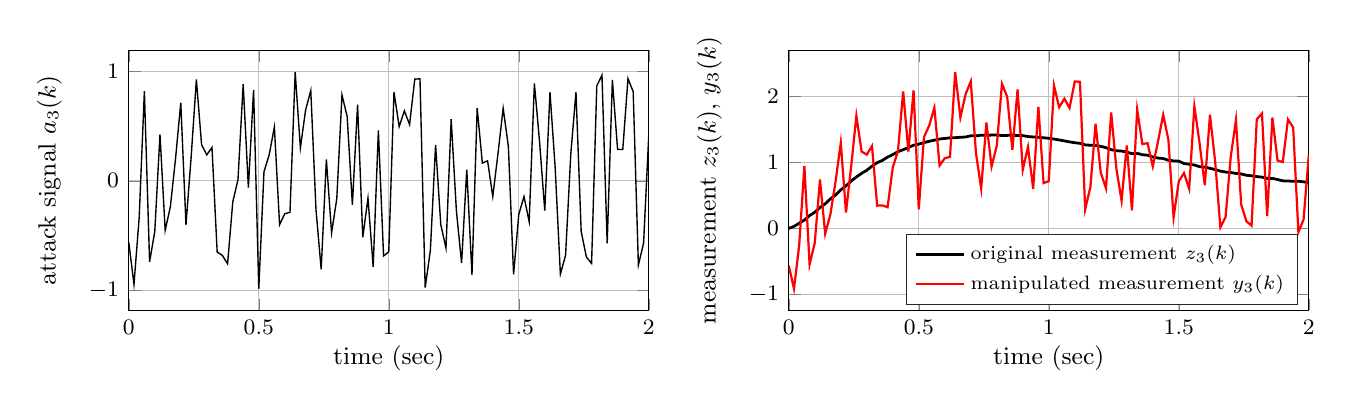
\begin{tikzpicture}
\begin{axis}
[	width=2.6in,
	height=1.3in,
	at={(0in,1.7in)},
	scale only axis,
	xmin=0,
	xmax=2.0,
	xlabel={\small time (sec)},
	ylabel={\small attack signal $a_3(k)$},
	x label style={at={(axis description cs:0.5,-0.1)},anchor=north},
	y label style={at={(axis description cs:-0.11,.5)},anchor=south},
	xticklabel style = {font=\footnotesize},
	yticklabel style = {font=\footnotesize},
	axis background/.style={fill=white},
	xmajorgrids,
	ymajorgrids,
	legend style={at={(0.98,0.02)}, anchor=south east, legend cell align=left, align=left, draw=white!15!black, font=\scriptsize}]
	 \addplot [color={black}, line width=0.5pt]
	table[row sep={\\}]
	{
0.0  -0.5625685225246384  \\
0.02  -0.946157670457147  \\
0.04  -0.3364104982135254  \\
0.06  0.8202072091057051  \\
0.08  -0.7416794304773182  \\
0.1  -0.4636695887925457  \\
0.12  0.4247375003814464  \\
0.14  -0.4529398288478932  \\
0.16  -0.23609426388419186  \\
0.18  0.20607156940463156  \\
0.2  0.7146776978338217  \\
0.22  -0.4031811551171538  \\
0.24  0.2206252826036046  \\
0.26  0.9264480578446211  \\
0.28  0.33016511715381247  \\
0.3  0.23718509653538966  \\
0.32  0.3053190945443012  \\
0.34  -0.6512496890635018  \\
0.36  -0.6822150171560071  \\
0.38  -0.7591862879712541  \\
0.4  -0.19280907417578508  \\
0.42  0.010038743472394973  \\
0.44  0.8827731819816345  \\
0.46  -0.06232326649906916  \\
0.48  0.8319345169225183  \\
0.5  -0.9872827034407057  \\
0.52  0.08252119515841416  \\
0.54  0.23761861917437788  \\
0.56  0.4911335147891096  \\
0.58  -0.40195620239799457  \\
0.6  -0.3007915416907321  \\
0.62  -0.2880389885558321  \\
0.64  0.9936238737504954  \\
0.66  0.301057855330896  \\
0.68  0.6458920116460922  \\
0.7  0.825439900787106  \\
0.72  -0.2620778554704919  \\
0.74  -0.8099631243406966  \\
0.76  0.19437015142373726  \\
0.78  -0.4755865591670845  \\
0.8  -0.16394509461018458  \\
0.82  0.7845865898376772  \\
0.84  0.5867174223091793  \\
0.86  -0.2193032349255386  \\
0.88  0.6958595916418464  \\
0.9  -0.5164339756771317  \\
0.92  -0.15836646301569557  \\
0.94  -0.7857843469695074  \\
0.96  0.46132582292170277  \\
0.98  -0.6869516269713491  \\
1.0  -0.6493852750653204  \\
1.02  0.8112005067738504  \\
1.04  0.49552013490097657  \\
1.06  0.6395260827687634  \\
1.08  0.5144317327991712  \\
1.1  0.9294456667948578  \\
1.12  0.9324288820292381  \\
1.14  -0.9769366346964161  \\
1.16  -0.6351510189600362  \\
1.18  0.32726158838108965  \\
1.2  -0.40098100760181365  \\
1.22  -0.6150064270922488  \\
1.24  0.5641016529988976  \\
1.26  -0.27231215515339535  \\
1.28  -0.752554332947537  \\
1.3  0.10187427646239922  \\
1.32  -0.8600011844841662  \\
1.34  0.6642700257000524  \\
1.36  0.16170120198315496  \\
1.38  0.1826664933681159  \\
1.4  -0.14334483866806247  \\
1.42  0.2486222622627241  \\
1.44  0.6622426969022284  \\
1.46  0.3136861979015393  \\
1.48  -0.8557620863445856  \\
1.5  -0.3070342555493415  \\
1.52  -0.14416760270375484  \\
1.54  -0.37368830515195883  \\
1.56  0.8911874844829586  \\
1.58  0.35518376316127453  \\
1.6  -0.27339031973850947  \\
1.62  0.8105521223144891  \\
1.64  0.11784059265095037  \\
1.66  -0.8529040350736259  \\
1.68  -0.6806944273502968  \\
1.7  0.24363510423789958  \\
1.72  0.8110402429453711  \\
1.74  -0.4624898957872765  \\
1.76  -0.6967699885218077  \\
1.78  -0.7555009870069109  \\
1.8  0.8677999951918474  \\
1.82  0.9651388566369782  \\
1.84  -0.572692343156155  \\
1.86  0.9214722802132305  \\
1.88  0.28714732919033314  \\
1.9  0.28600006541082534  \\
1.92  0.9336419255406856  \\
1.94  0.8153373412752746  \\
1.96  -0.771121795555112  \\
1.98  -0.5703813934558002  \\
2.0  0.4202296393480983  \\
	};
	

\end{axis}

\begin{axis}
[	width=2.6in,
height=1.3in,
at={(3.3in,1.7in)},
scale only axis,
xmin=0,
xmax=2.0,
xlabel={\small time (sec)},
ylabel={\small measurement $z_3(k)$, $y_3(k)$},
x label style={at={(axis description cs:0.5,-0.1)},anchor=north},
y label style={at={(axis description cs:-0.11,.5)},anchor=south},
xticklabel style = {font=\footnotesize},
yticklabel style = {font=\footnotesize},
axis background/.style={fill=white},
xmajorgrids,
ymajorgrids,
legend style={at={(0.98,0.02)}, anchor=south east, legend cell align=left, align=left, draw=white!15!black, font=\scriptsize}]
\addplot [color={black}, line width=1pt]
table[row sep={\\}]
{
	0.0  0.0005061476188890966  \\
	0.02  0.031676588671764164  \\
	0.04  0.07839140216717005  \\
	0.06  0.12705814413038907  \\
	0.08  0.19480431491342415  \\
	0.1  0.24606443660984756  \\
	0.12  0.3172084112413346  \\
	0.14  0.3736461521457517  \\
	0.16  0.44787503073264906  \\
	0.18  0.5069223027691104  \\
	0.2  0.5852364000596318  \\
	0.22  0.6450996948371481  \\
	0.24  0.719598187094292  \\
	0.26  0.7802246068858262  \\
	0.28  0.8352976511484314  \\
	0.3  0.8819249843701404  \\
	0.32  0.9438334235786126  \\
	0.34  0.9968137130862087  \\
	0.36  1.0315121996566714  \\
	0.38  1.081352724577131  \\
	0.4  1.1186852002911756  \\
	0.42  1.1641077812910212  \\
	0.44  1.1939659134273448  \\
	0.46  1.2272556361330376  \\
	0.48  1.261665715825486  \\
	0.5  1.2786078316998268  \\
	0.52  1.3011683448134117  \\
	0.54  1.321384821506629  \\
	0.56  1.338382036174266  \\
	0.58  1.355281400342649  \\
	0.6  1.3648091021791213  \\
	0.62  1.3732953101805965  \\
	0.64  1.3762112690389299  \\
	0.66  1.382112031788601  \\
	0.68  1.3860206445448202  \\
	0.7  1.4048404930230238  \\
	0.72  1.4039269899470739  \\
	0.74  1.4137690804441447  \\
	0.76  1.4113935296580151  \\
	0.78  1.415466288691426  \\
	0.8  1.4173504637099132  \\
	0.82  1.408216099780143  \\
	0.84  1.410853101252453  \\
	0.86  1.4122366732375526  \\
	0.88  1.4099148151176653  \\
	0.9  1.4068220459084428  \\
	0.92  1.3932771447410874  \\
	0.94  1.3869197810882306  \\
	0.96  1.3816719911696593  \\
	0.98  1.3746540193141819  \\
	1.0  1.3668281178807369  \\
	1.02  1.3552820898141782  \\
	1.04  1.3412950137254243  \\
	1.06  1.327392873379449  \\
	1.08  1.312190740537211  \\
	1.1  1.2995220178320626  \\
	1.12  1.290181413888831  \\
	1.14  1.2667219743156652  \\
	1.16  1.2612298991666215  \\
	1.18  1.2589715517767963  \\
	1.2  1.2447068247074753  \\
	1.22  1.2246558090903343  \\
	1.24  1.1947392767545253  \\
	1.26  1.178691587432372  \\
	1.28  1.1725210952749316  \\
	1.3  1.1574143114167688  \\
	1.32  1.1333554895621063  \\
	1.34  1.1379319746939296  \\
	1.36  1.1176217433173101  \\
	1.38  1.1102593716696092  \\
	1.4  1.0836873054208704  \\
	1.42  1.067036714947158  \\
	1.44  1.0605533729454986  \\
	1.46  1.0344992068703907  \\
	1.48  1.0243303238705184  \\
	1.5  1.020077500634661  \\
	1.52  0.9839768264319667  \\
	1.54  0.973260433229496  \\
	1.56  0.9617053886606732  \\
	1.58  0.936138032340902  \\
	1.6  0.9293793225658402  \\
	1.62  0.9117291638631297  \\
	1.64  0.8920858206651604  \\
	1.66  0.8695958676647998  \\
	1.68  0.8548008571060354  \\
	1.7  0.8475448183415518  \\
	1.72  0.8342039556123342  \\
	1.74  0.8264765990017806  \\
	1.76  0.806244182872368  \\
	1.78  0.798659029368042  \\
	1.8  0.7863949401958488  \\
	1.82  0.7781995154823723  \\
	1.84  0.7591860534071165  \\
	1.86  0.7588840404102928  \\
	1.88  0.7418834336133863  \\
	1.9  0.7215463501855689  \\
	1.92  0.7193921889269146  \\
	1.94  0.714570339094586  \\
	1.96  0.7160728188691623  \\
	1.98  0.7071802256678278  \\
	2.0  0.6911892058577479  \\
}
;\addlegendentry{original measurement $z_3(k)$}

\addplot [color={red}, line width=0.8pt]
table[row sep={\\}]
{
   0.0  -0.5620623749057493  \\
0.02  -0.9144810817853829  \\
0.04  -0.25801909604635537  \\
0.06  0.9472653532360942  \\
0.08  -0.546875115563894  \\
0.1  -0.21760515218269816  \\
0.12  0.741945911622781  \\
0.14  -0.07929367670214149  \\
0.16  0.2117807668484572  \\
0.18  0.712993872173742  \\
0.2  1.2999140978934536  \\
0.22  0.24191853971999433  \\
0.24  0.9402234696978966  \\
0.26  1.7066726647304473  \\
0.28  1.1654627683022438  \\
0.3  1.11911008090553  \\
0.32  1.2491525181229137  \\
0.34  0.3455640240227069  \\
0.36  0.3492971825006643  \\
0.38  0.32216643660587696  \\
0.4  0.9258761261153905  \\
0.42  1.1741465247634162  \\
0.44  2.0767390954089793  \\
0.46  1.1649323696339684  \\
0.48  2.0936002327480043  \\
0.5  0.29132512825912116  \\
0.52  1.3836895399718259  \\
0.54  1.559003440681007  \\
0.56  1.8295155509633756  \\
0.58  0.9533251979446544  \\
0.6  1.0640175604883892  \\
0.62  1.0852563216247644  \\
0.64  2.3698351427894253  \\
0.66  1.683169887119497  \\
0.68  2.0319126561909124  \\
0.7  2.23028039381013  \\
0.72  1.141849134476582  \\
0.74  0.6038059561034481  \\
0.76  1.6057636810817524  \\
0.78  0.9398797295243415  \\
0.8  1.2534053690997287  \\
0.82  2.19280268961782  \\
0.84  1.9975705235616323  \\
0.86  1.192933438312014  \\
0.88  2.1057744067595117  \\
0.9  0.8903880702313112  \\
0.92  1.2349106817253919  \\
0.94  0.6011354341187232  \\
0.96  1.842997814091362  \\
0.98  0.6877023923428327  \\
1.0  0.7174428428154165  \\
1.02  2.1664825965880286  \\
1.04  1.8368151486264008  \\
1.06  1.9669189561482123  \\
1.08  1.8266224733363823  \\
1.1  2.2289676846269204  \\
1.12  2.222610295918069  \\
1.14  0.2897853396192491  \\
1.16  0.6260788802065853  \\
1.18  1.586233140157886  \\
1.2  0.8437258171056616  \\
1.22  0.6096493819980855  \\
1.24  1.7588409297534229  \\
1.26  0.9063794322789767  \\
1.28  0.4199667623273946  \\
1.3  1.259288587879168  \\
1.32  0.2733543050779401  \\
1.34  1.802202000393982  \\
1.36  1.279322945300465  \\
1.38  1.292925865037725  \\
1.4  0.940342466752808  \\
1.42  1.3156589772098821  \\
1.44  1.722796069847727  \\
1.46  1.34818540477193  \\
1.48  0.16856823752593275  \\
1.5  0.7130432450853195  \\
1.52  0.8398092237282119  \\
1.54  0.5995721280775371  \\
1.56  1.8528928731436318  \\
1.58  1.2913217955021765  \\
1.6  0.6559890028273307  \\
1.62  1.7222812861776189  \\
1.64  1.0099264133161108  \\
1.66  0.016691832591173905  \\
1.68  0.17410642975573853  \\
1.7  1.0911799225794514  \\
1.72  1.6452441985577053  \\
1.74  0.3639867032145041  \\
1.76  0.10947419435056027  \\
1.78  0.04315804236113108  \\
1.8  1.6541949353876961  \\
1.82  1.7433383721193505  \\
1.84  0.1864937102509615  \\
1.86  1.6803563206235232  \\
1.88  1.0290307628037194  \\
1.9  1.0075464155963942  \\
1.92  1.6530341144676002  \\
1.94  1.5299076803698606  \\
1.96  -0.05504897668594966  \\
1.98  0.1367988322120276  \\
2.0  1.1114188452058462  \\
}
;\addlegendentry{{manipulated measurement $y_3(k)$}}


\end{axis}

%  	\begin{axis}
%	[	width=2.6in,
%	height=1.3in,
%	at={(0in,0in)},
%	scale only axis,
%	xmin=0,
%	xmax=2.0,
%%	ymin=-4,
%%	ymax=2,
%	xlabel={\small time (sec)},
%	ylabel={\small $x_3$ pendulumn angle},
%	x label style={at={(axis description cs:0.5,-0.1)},anchor=north},
%	y label style={at={(axis description cs:-0.11,.5)},anchor=south},
%	xticklabel style = {font=\footnotesize},
%	yticklabel style = {font=\footnotesize},
%	axis background/.style={fill=white},
%	xmajorgrids,
%	ymajorgrids,
%	legend style={at={(0.98,0.02)}, anchor=south east, legend cell align=left, align=left, draw=white!15!black, font=\scriptsize}]
%	\addplot [color={black}, line width=1pt]
%	table[row sep={\\}]
%	{
%0.0  0.0  \\
%0.02  0.00772853593415913  \\
%0.04  0.004801671416923327  \\
%0.06  -0.012528997431996048  \\
%0.08  -0.034478619332425936  \\
%0.1  -0.06220231524500317  \\
%0.12  -0.08812635048651297  \\
%0.14  -0.11408845091735348  \\
%0.16  -0.14488997218330013  \\
%0.18  -0.16947348245078697  \\
%0.2  -0.19501471373927462  \\
%0.22  -0.2166030568036244  \\
%0.24  -0.23694887645664164  \\
%0.26  -0.2534179553657174  \\
%0.28  -0.2659048131170473  \\
%0.3  -0.2814074322954603  \\
%0.32  -0.2947651384686937  \\
%0.34  -0.30280625979339526  \\
%0.36  -0.3110461733895194  \\
%0.38  -0.322599925444607  \\
%0.4  -0.3266601375700984  \\
%0.42  -0.32832183302190043  \\
%0.44  -0.33079378651792585  \\
%0.46  -0.33139999061403563  \\
%0.48  -0.33190912976035625  \\
%0.5  -0.32830514918189446  \\
%0.52  -0.3265624628054656  \\
%0.54  -0.3231032971609128  \\
%0.56  -0.31943423376946206  \\
%0.58  -0.31567219360956844  \\
%0.6  -0.3139459878003922  \\
%0.62  -0.30858429971742735  \\
%0.64  -0.302866065490615  \\
%0.66  -0.2975240107704187  \\
%0.68  -0.29156813130488785  \\
%0.7  -0.28705864201984305  \\
%0.72  -0.2800613967051828  \\
%0.74  -0.2721345042496352  \\
%0.76  -0.2675647476463787  \\
%0.78  -0.26004373544306775  \\
%0.8  -0.24895562242482422  \\
%0.82  -0.24469615255703123  \\
%0.84  -0.23679296240647962  \\
%0.86  -0.22526462977535064  \\
%0.88  -0.21530137387528134  \\
%0.9  -0.2019610820610649  \\
%0.92  -0.19283115640996426  \\
%0.94  -0.18404650174938508  \\
%0.96  -0.1761938176509628  \\
%0.98  -0.16952154188571567  \\
%1.0  -0.16068318494400077  \\
%1.02  -0.15115385465801076  \\
%1.04  -0.142077499764086  \\
%1.06  -0.13285231555738442  \\
%1.08  -0.12217488148841449  \\
%1.1  -0.11717625074624005  \\
%1.12  -0.11014342489808715  \\
%1.14  -0.10290962697247244  \\
%1.16  -0.09707223606283309  \\
%1.18  -0.08535583686102192  \\
%1.2  -0.07985586728850495  \\
%1.22  -0.07053290137389215  \\
%1.24  -0.0660756875734225  \\
%1.26  -0.05925950423578198  \\
%1.28  -0.04983238664926049  \\
%1.3  -0.046321730532286276  \\
%1.32  -0.04111947230774583  \\
%1.34  -0.03716014124124552  \\
%1.36  -0.026958173254637667  \\
%1.38  -0.02105479624823502  \\
%1.4  -0.013204082238369545  \\
%1.42  -0.007208612852129617  \\
%1.44  -0.005029793064317797  \\
%1.46  -0.0030365387904538444  \\
%1.48  -0.004685191023569348  \\
%1.5  -0.0013502134977833556  \\
%1.52  -0.0012637857934116841  \\
%1.54  -0.0012840803221537893  \\
%1.56  0.004161592495718868  \\
%1.58  0.007337270321035059  \\
%1.6  0.007873265952081725  \\
%1.62  0.007756595504494869  \\
%1.64  0.012948213825993315  \\
%1.66  0.01713997304166258  \\
%1.68  0.019303428528959714  \\
%1.7  0.021720664071569973  \\
%1.72  0.021496525088056485  \\
%1.74  0.02269954427453162  \\
%1.76  0.025127263635035712  \\
%1.78  0.025581388241573386  \\
%1.8  0.022956371536018347  \\
%1.82  0.020320909246699284  \\
%1.84  0.02325727363447171  \\
%1.86  0.022566429135964905  \\
%1.88  0.025410932971556357  \\
%1.9  0.025581397517493814  \\
%1.92  0.024133015365711413  \\
%1.94  0.024607306183292644  \\
%1.96  0.02686997993370564  \\
%1.98  0.028618584557972122  \\
%2.0  0.02949612536857937  \\
%	}
%	;\addlegendentry{state $x_3$}
%	\addplot [color={red},dashed, line width=1pt]
%	table[row sep={\\}]
%	{
%	 0.0  0.0  \\
%	0.02  0.00809402453328914  \\
%	0.04  0.002283710058266839  \\
%	0.06  -0.011924222353404363  \\
%	0.08  -0.03538807548199385  \\
%	0.1  -0.062495688561897404  \\
%	0.12  -0.08979727756857352  \\
%	0.14  -0.11596912737252132  \\
%	0.16  -0.14427298978459968  \\
%	0.18  -0.1699091880689923  \\
%	0.2  -0.19571409358693093  \\
%	0.22  -0.21710723871475957  \\
%	0.24  -0.23750518798723996  \\
%	0.26  -0.2523487237267693  \\
%	0.28  -0.26564551359739796  \\
%	0.3  -0.28113924184632594  \\
%	0.32  -0.29344313265186917  \\
%	0.34  -0.30387742299429843  \\
%	0.36  -0.31093266172634626  \\
%	0.38  -0.32032314034771303  \\
%	0.4  -0.32488432492231156  \\
%	0.42  -0.328256133800731  \\
%	0.44  -0.33170684466667966  \\
%	0.46  -0.33284554813223155  \\
%	0.48  -0.32934060251669267  \\
%	0.5  -0.32881415681358606  \\
%	0.52  -0.32672393145274836  \\
%	0.54  -0.3217023284966502  \\
%	0.56  -0.31920782046530927  \\
%	0.58  -0.3155857583713461  \\
%	0.6  -0.31200171978648444  \\
%	0.62  -0.30753884981430435  \\
%	0.64  -0.30328744734313084  \\
%	0.66  -0.298819639225292  \\
%	0.68  -0.2916263924411364  \\
%	0.7  -0.2838538399639527  \\
%	0.72  -0.27822533107121034  \\
%	0.74  -0.27214850374295424  \\
%	0.76  -0.2649862125224101  \\
%	0.78  -0.2581935349054245  \\
%	0.8  -0.24687375692743166  \\
%	0.82  -0.24215334598492766  \\
%	0.84  -0.23463968652823464  \\
%	0.86  -0.2266454648618093  \\
%	0.88  -0.21570653361944153  \\
%	0.9  -0.20378113555698663  \\
%	0.92  -0.1922094272504351  \\
%	0.94  -0.18193892229656553  \\
%	0.96  -0.17462306148804935  \\
%	0.98  -0.16857998362472904  \\
%	1.0  -0.1589098101915298  \\
%	1.02  -0.1502282447377052  \\
%	1.04  -0.14310208638808308  \\
%	1.06  -0.13391428982914821  \\
%	1.08  -0.12206666034954945  \\
%	1.1  -0.11753381580332939  \\
%	1.12  -0.11064111898353321  \\
%	1.14  -0.10215982660161821  \\
%	1.16  -0.096618902112179  \\
%	1.18  -0.08817640412095815  \\
%	1.2  -0.07931844432254224  \\
%	1.22  -0.0713170158403937  \\
%	1.24  -0.06598326032462205  \\
%	1.26  -0.05869782541506201  \\
%	1.28  -0.05244831403760163  \\
%	1.3  -0.04689123976106053  \\
%	1.32  -0.04325454089798624  \\
%	1.34  -0.03885220256504527  \\
%	1.36  -0.030517495413270805  \\
%	1.38  -0.024466342268987945  \\
%	1.4  -0.018729185184462  \\
%	1.42  -0.010157661361933055  \\
%	1.44  -0.005799650225733364  \\
%	1.46  -0.0017710381011364653  \\
%	1.48  -0.002224799382994183  \\
%	1.5  -0.0037629560253844437  \\
%	1.52  -0.00020440203585928116  \\
%	1.54  0.0012643359647233753  \\
%	1.56  0.003252784378121404  \\
%	1.58  0.005266412443152401  \\
%	1.6  0.006949937595322902  \\
%	1.62  0.008256452575278935  \\
%	1.64  0.012007453507124496  \\
%	1.66  0.01615310418726861  \\
%	1.68  0.019000666804788804  \\
%	1.7  0.022087371511188413  \\
%	1.72  0.022261092399250972  \\
%	1.74  0.02355749395802008  \\
%	1.76  0.023895346270558754  \\
%	1.78  0.026333022304786253  \\
%	1.8  0.02456626556539792  \\
%	1.82  0.021605386228436392  \\
%	1.84  0.023528349423668403  \\
%	1.86  0.023572743261476937  \\
%	1.88  0.025126899283551846  \\
%	1.9  0.025833933274513415  \\
%	1.92  0.02280935517999988  \\
%	1.94  0.025189469054832925  \\
%	1.96  0.02661138935665535  \\
%	1.98  0.02763011362829756  \\
%	2.0  0.027469141828147026  \\
%	}
%	;\addlegendentry{{ Kalman estimation $\hat{x}_3$}}
%	\addplot[densely dotted, color={blue}, line width=1pt]
%	table[row sep={\\}]
%	{
%    0.0  1.8153964737662312e-5  \\
%0.02  0.0066894619554046355  \\
%0.04  0.0018375871994040162  \\
%0.06  -0.011012697570773474  \\
%0.08  -0.03609804873935931  \\
%0.1  -0.06340645502442915  \\
%0.12  -0.0895457918792631  \\
%0.14  -0.11546107462068377  \\
%0.16  -0.14461477831571443  \\
%0.18  -0.17007154514361927  \\
%0.2  -0.1965051643232883  \\
%0.22  -0.2166340902306285  \\
%0.24  -0.23770039325448397  \\
%0.26  -0.2507335125541037  \\
%0.28  -0.2645156857629006  \\
%0.3  -0.28216527675191616  \\
%0.32  -0.2939902057265568  \\
%0.34  -0.30440857374041375  \\
%0.36  -0.31047444062583235  \\
%0.38  -0.32198495278139255  \\
%0.4  -0.3249118700086211  \\
%0.42  -0.32841640163734204  \\
%0.44  -0.33251010788936297  \\
%0.46  -0.3331188005365526  \\
%0.48  -0.32767165979082796  \\
%0.5  -0.3288637216034393  \\
%0.52  -0.3265504673964966  \\
%0.54  -0.3205275268798475  \\
%0.56  -0.3197884422608594  \\
%0.58  -0.3157679939079811  \\
%0.6  -0.31254421435944685  \\
%0.62  -0.30806083114358135  \\
%0.64  -0.3038352148338218  \\
%0.66  -0.2994116819525727  \\
%0.68  -0.29121889287466646  \\
%0.7  -0.2833617882231757  \\
%0.72  -0.27936861590095097  \\
%0.74  -0.27290542088826425  \\
%0.76  -0.2654318394097727  \\
%0.78  -0.25942935600796185  \\
%0.8  -0.2457658293296008  \\
%0.82  -0.24403414344605018  \\
%0.84  -0.2358616914531913  \\
%0.86  -0.2275077308550984  \\
%0.88  -0.21485981313066116  \\
%0.9  -0.20232178782749977  \\
%0.92  -0.19104608352709898  \\
%0.94  -0.18111885006671183  \\
%0.96  -0.1754534261052666  \\
%0.98  -0.17003134488456753  \\
%1.0  -0.15878283143959224  \\
%1.02  -0.15051065091807594  \\
%1.04  -0.1435009071579159  \\
%1.06  -0.13363074186982313  \\
%1.08  -0.12038778178826819  \\
%1.1  -0.11866338138681089  \\
%1.12  -0.110930248968576  \\
%1.14  -0.10181163345285733  \\
%1.16  -0.09751700179946482  \\
%1.18  -0.08758702035485068  \\
%1.2  -0.07785509840417323  \\
%1.22  -0.07050311362538186  \\
%1.24  -0.06601841440192815  \\
%1.26  -0.05793710743206526  \\
%1.28  -0.051999353311811235  \\
%1.3  -0.04693730475850037  \\
%1.32  -0.04389217870983184  \\
%1.34  -0.038972560152190514  \\
%1.36  -0.02865888152011623  \\
%1.38  -0.02353592133370778  \\
%1.4  -0.017640744192343967  \\
%1.42  -0.007667707763960579  \\
%1.44  -0.004952961222438092  \\
%1.46  -0.0008037137317556581  \\
%1.48  -0.003445327891030425  \\
%1.5  -0.005518722706033974  \\
%1.52  0.0004546477429451413  \\
%1.54  0.0010515168391628813  \\
%1.56  0.0032978681139044274  \\
%1.58  0.005456467908684386  \\
%1.6  0.007016058115342972  \\
%1.62  0.007992613905111441  \\
%1.64  0.013215471326015648  \\
%1.66  0.01730891328170967  \\
%1.68  0.01980891940823777  \\
%1.7  0.023250483613783467  \\
%1.72  0.02194819975361911  \\
%1.74  0.023940958356646756  \\
%1.76  0.023721571245686246  \\
%1.78  0.027350023652804832  \\
%1.8  0.023546924861985615  \\
%1.82  0.019857344070720775  \\
%1.84  0.023909886569047793  \\
%1.86  0.0231294380862511  \\
%1.88  0.02574352864188202  \\
%1.9  0.025842587721728108  \\
%1.92  0.02092146538831675  \\
%1.94  0.025931184643444655  \\
%1.96  0.027084411024922466  \\
%1.98  0.027575839585923738  \\
%2.0  0.026971498895954696  \\
%	}
%;\addlegendentry{{our estimation $\tilde{x}_3$}}
%
%
%\end{axis}
%
%\begin{axis}
%[	width=2.6in,
%height=1.3in,
%at={(3.3in,0in)},
%scale only axis,
%xmin=0,
%xmax=2.0,
%%ymin=-4,
%%ymax=2,
%xlabel={\small time (sec)},
%ylabel={\small $x_4$ pendulumn angle velocity},
%x label style={at={(axis description cs:0.5,-0.1)},anchor=north},
%y label style={at={(axis description cs:-0.11,.5)},anchor=south},
%xticklabel style = {font=\footnotesize},
%yticklabel style = {font=\footnotesize},
%axis background/.style={fill=white},
%xmajorgrids,
%ymajorgrids,
%legend style={at={(0.98,0.02)}, anchor=south east, legend cell align=left, align=left, draw=white!15!black, font=\scriptsize}]
%\addplot [color={black}, line width=1pt]
%table[row sep={\\}]
%{
%  0.0  1.0  \\
%0.02  0.05313305390126177  \\
%0.04  -0.5807597079886778  \\
%0.06  -0.9849649892184913  \\
%0.08  -1.2236616544745775  \\
%0.1  -1.3448708265564777  \\
%0.12  -1.3911973425235322  \\
%0.14  -1.3847017109780744  \\
%0.16  -1.3360588370385862  \\
%0.18  -1.2612956960549269  \\
%0.2  -1.1712121233640451  \\
%0.22  -1.071999578445813  \\
%0.24  -0.9674797110228057  \\
%0.26  -0.8680549183886634  \\
%0.28  -0.7699884280336178  \\
%0.3  -0.6746842796248621  \\
%0.32  -0.586875654761506  \\
%0.34  -0.4959299174041296  \\
%0.36  -0.40597661697079446  \\
%0.38  -0.32771095994654365  \\
%0.4  -0.253961547290701  \\
%0.42  -0.18263871652089975  \\
%0.44  -0.11573407741218594  \\
%0.46  -0.05911515161120641  \\
%0.48  0.0009801138197992887  \\
%0.5  0.04463813200237973  \\
%0.52  0.09038368590143643  \\
%0.54  0.12381466371390598  \\
%0.56  0.16193471899976158  \\
%0.58  0.19217803962499197  \\
%0.6  0.2284585486584002  \\
%0.62  0.27315223526991256  \\
%0.64  0.3029744279918313  \\
%0.66  0.3360381761463694  \\
%0.68  0.36405311581028843  \\
%0.7  0.3862145241118462  \\
%0.72  0.4052381391063923  \\
%0.74  0.40659407112164414  \\
%0.76  0.4016463115722345  \\
%0.78  0.39680426743202124  \\
%0.8  0.3921338510569967  \\
%0.82  0.3884591608505884  \\
%0.84  0.3897778445333768  \\
%0.86  0.3978434385510643  \\
%0.88  0.40888248291393214  \\
%0.9  0.40349125898703586  \\
%0.92  0.4043181979298124  \\
%0.94  0.4001713487291486  \\
%0.96  0.397537790317619  \\
%0.98  0.3906342747298136  \\
%1.0  0.377882856254513  \\
%1.02  0.3727858562415341  \\
%1.04  0.3579748382263377  \\
%1.06  0.34457979003538486  \\
%1.08  0.3274365776280705  \\
%1.1  0.31223393396172927  \\
%1.12  0.2972605478138003  \\
%1.14  0.28374482940224277  \\
%1.16  0.27808313315371463  \\
%1.18  0.2752540519763583  \\
%1.2  0.27226461109496636  \\
%1.22  0.27696110635321103  \\
%1.24  0.26990768271144283  \\
%1.26  0.26054532527838425  \\
%1.28  0.2504740216554849  \\
%1.3  0.24312004848395827  \\
%1.32  0.24828658502523776  \\
%1.34  0.2471687742404289  \\
%1.36  0.2483512476352048  \\
%1.38  0.2421106054905815  \\
%1.4  0.2281155213543221  \\
%1.42  0.2192043397969218  \\
%1.44  0.21813440821530206  \\
%1.46  0.215847499113375  \\
%1.48  0.21810640903792972  \\
%1.5  0.21793606071633792  \\
%1.52  0.21839791991053367  \\
%1.54  0.21094224607272868  \\
%1.56  0.20175648284456538  \\
%1.58  0.18577552098976302  \\
%1.6  0.17234252915874954  \\
%1.62  0.1667589628096436  \\
%1.64  0.16336600936391402  \\
%1.66  0.15026901018454916  \\
%1.68  0.1427360828668787  \\
%1.7  0.13367410170858618  \\
%1.72  0.12734499958354706  \\
%1.74  0.11405351681196844  \\
%1.76  0.10587244286568445  \\
%1.78  0.10156266429081387  \\
%1.8  0.0936679758808678  \\
%1.82  0.08822122445956102  \\
%1.84  0.07018133601995245  \\
%1.86  0.05094537909202273  \\
%1.88  0.04130087142500513  \\
%1.9  0.032313361980953  \\
%1.92  0.02866897811479254  \\
%1.94  0.030018199155337016  \\
%1.96  0.029179914657290675  \\
%1.98  0.029178093401201616  \\
%2.0  0.02640041419686011  \\
%}
%;\addlegendentry{state $x_4$}
%\addplot [color={red},dashed, line width=1pt]
%table[row sep={\\}]
%{
%0.0  1.0  \\
%0.02  0.05196229099537668  \\
%0.04  -0.5824313535988286  \\
%0.06  -0.9891377715191895  \\
%0.08  -1.225040556372666  \\
%0.1  -1.3474376677420603  \\
%0.12  -1.3927650448471267  \\
%0.14  -1.3853875418228592  \\
%0.16  -1.3385535189542455  \\
%0.18  -1.2616908106226903  \\
%0.2  -1.1733481356619362  \\
%0.22  -1.0733971982561636  \\
%0.24  -0.9709048883726853  \\
%0.26  -0.8734509930998627  \\
%0.28  -0.7737477786715035  \\
%0.3  -0.6814462079764667  \\
%0.32  -0.5930068323706987  \\
%0.34  -0.5011111690344067  \\
%0.36  -0.4117486708366517  \\
%0.38  -0.32787217975647187  \\
%0.4  -0.25500615240975977  \\
%0.42  -0.18223637558459482  \\
%0.44  -0.1136859116043202  \\
%0.46  -0.05435490540626656  \\
%0.48  0.001052155333388885  \\
%0.5  0.047862836014496535  \\
%0.52  0.09307612385402939  \\
%0.54  0.12661541422593295  \\
%0.56  0.16673898540858903  \\
%0.58  0.20040364092746082  \\
%0.6  0.2378257684031066  \\
%0.62  0.28092995786664526  \\
%0.64  0.30722850104675375  \\
%0.66  0.33988761950874746  \\
%0.68  0.3717014698259486  \\
%0.7  0.39114473419457757  \\
%0.72  0.41074056965705785  \\
%0.74  0.4157082365437478  \\
%0.76  0.4107206907578836  \\
%0.78  0.40479797621004415  \\
%0.8  0.4002479612239634  \\
%0.82  0.39670525295180864  \\
%0.84  0.402980720989716  \\
%0.86  0.40966660580558506  \\
%0.88  0.41939855229643713  \\
%0.9  0.4136774603389678  \\
%0.92  0.41337706589827294  \\
%0.94  0.4076360923733703  \\
%0.96  0.40419133912255345  \\
%0.98  0.39738214224816115  \\
%1.0  0.38613613596819135  \\
%1.02  0.37863833492291044  \\
%1.04  0.3613171630485197  \\
%1.06  0.34817084130208276  \\
%1.08  0.3337665386001098  \\
%1.1  0.322513876054837  \\
%1.12  0.30951293238535926  \\
%1.14  0.29822140789925367  \\
%1.16  0.2887209415996951  \\
%1.18  0.2855447198327156  \\
%1.2  0.2792019100681843  \\
%1.22  0.28259480121327957  \\
%1.24  0.27674766540821855  \\
%1.26  0.2679337895584435  \\
%1.28  0.25957147095312993  \\
%1.3  0.2512852868921737  \\
%1.32  0.25335034594023265  \\
%1.34  0.2517049563980485  \\
%1.36  0.24854241554762116  \\
%1.38  0.2437570887642059  \\
%1.4  0.232081337423728  \\
%1.42  0.2246763936573522  \\
%1.44  0.22593853025256636  \\
%1.46  0.22180580292165525  \\
%1.48  0.2201777881736648  \\
%1.5  0.21772174841998373  \\
%1.52  0.22039359761167476  \\
%1.54  0.21451665272588324  \\
%1.56  0.20671496543671092  \\
%1.58  0.19237907013470915  \\
%1.6  0.17849341727408496  \\
%1.62  0.1693669711801831  \\
%1.64  0.1654694365161853  \\
%1.66  0.15476608715270937  \\
%1.68  0.14644491458503275  \\
%1.7  0.1380087312073818  \\
%1.72  0.12999696162763208  \\
%1.74  0.11642996712779241  \\
%1.76  0.10651977489569771  \\
%1.78  0.09914327961373791  \\
%1.8  0.09326070775598083  \\
%1.82  0.08760116773835838  \\
%1.84  0.07441328030636729  \\
%1.86  0.0534154762075595  \\
%1.88  0.04537417203289343  \\
%1.9  0.03311477519912949  \\
%1.92  0.029386264188961075  \\
%1.94  0.031449452742925314  \\
%1.96  0.028203792066178256  \\
%1.98  0.026902194874244584  \\
%2.0  0.023968301890876745  \\
%}
%;\addlegendentry{{ Kalman estimation $\hat{x}_4$}}
%\addplot[densely dotted, color={blue}, line width=1pt]
%table[row sep={\\}]
%{
%   0.0  0.9999999995931783  \\
%0.02  0.053256438469400355  \\
%0.04  -0.5810558367590097  \\
%0.06  -0.9888797959421549  \\
%0.08  -1.223881505907738  \\
%0.1  -1.3453082018539748  \\
%0.12  -1.3891303460776288  \\
%0.14  -1.379673068887711  \\
%0.16  -1.3337025957314825  \\
%0.18  -1.253342000372752  \\
%0.2  -1.165825320019194  \\
%0.22  -1.0647406851480974  \\
%0.24  -0.962864368017885  \\
%0.26  -0.8669013996514804  \\
%0.28  -0.7648147896002787  \\
%0.3  -0.6716102653407486  \\
%0.32  -0.5837308230993299  \\
%0.34  -0.49443467840184724  \\
%0.36  -0.40249690841846597  \\
%0.38  -0.3131891235819798  \\
%0.4  -0.2447579085019484  \\
%0.42  -0.17249116699733316  \\
%0.44  -0.1030719454933759  \\
%0.46  -0.04285668755265462  \\
%0.48  0.0114903655938736  \\
%0.5  0.058227653678667265  \\
%0.52  0.10717166963032067  \\
%0.54  0.1384072775498972  \\
%0.56  0.18001465974339406  \\
%0.58  0.2133703433896741  \\
%0.6  0.2465157229825645  \\
%0.62  0.28971937610144716  \\
%0.64  0.3129481166649311  \\
%0.66  0.3450497044394353  \\
%0.68  0.37686103961345435  \\
%0.7  0.3936878232730471  \\
%0.72  0.4150532260957958  \\
%0.74  0.4233531164511129  \\
%0.76  0.4171875013483728  \\
%0.78  0.41134854117958397  \\
%0.8  0.4070401399420528  \\
%0.82  0.39934970941532405  \\
%0.84  0.4045038112026713  \\
%0.86  0.41167154833883346  \\
%0.88  0.42410157171426555  \\
%0.9  0.4146297227803898  \\
%0.92  0.4139524638829347  \\
%0.94  0.40661075476522757  \\
%0.96  0.4036843661018631  \\
%0.98  0.39802668389530804  \\
%1.0  0.38824401885059434  \\
%1.02  0.38239487320383886  \\
%1.04  0.3633355958402282  \\
%1.06  0.35065780164947047  \\
%1.08  0.33821632861934037  \\
%1.1  0.3269686985664032  \\
%1.12  0.31461866216272727  \\
%1.14  0.30171518500382105  \\
%1.16  0.28963383826350086  \\
%1.18  0.2873988907364934  \\
%1.2  0.27659891830676514  \\
%1.22  0.2815743584939091  \\
%1.24  0.2796811226753734  \\
%1.26  0.2697498149899335  \\
%1.28  0.26134056909419723  \\
%1.3  0.24959006217362836  \\
%1.32  0.2504781981325628  \\
%1.34  0.24593217671946835  \\
%1.36  0.2426440319644277  \\
%1.38  0.24079990072853516  \\
%1.4  0.22929989748022161  \\
%1.42  0.22198397772499973  \\
%1.44  0.22259088456441103  \\
%1.46  0.21489558149696208  \\
%1.48  0.21275644734565288  \\
%1.5  0.20717683010408106  \\
%1.52  0.21169927725858503  \\
%1.54  0.20412663702544515  \\
%1.56  0.19746398862601647  \\
%1.58  0.1869741075430982  \\
%1.6  0.173740420161395  \\
%1.62  0.1604900026037437  \\
%1.64  0.15756553133036336  \\
%1.66  0.1481590395148509  \\
%1.68  0.13805716699049428  \\
%1.7  0.13040946307195095  \\
%1.72  0.12253183558288747  \\
%1.74  0.10883203724797469  \\
%1.76  0.09907761486652333  \\
%1.78  0.09264569886581496  \\
%1.8  0.08851705283528442  \\
%1.82  0.08454416975622558  \\
%1.84  0.07506523004933284  \\
%1.86  0.053058346159098005  \\
%1.88  0.04567485530664184  \\
%1.9  0.031371123950315244  \\
%1.92  0.02706214943933832  \\
%1.94  0.02810347265390892  \\
%1.96  0.024086348522412558  \\
%1.98  0.02104640638710214  \\
%2.0  0.021127296064900145  \\
%}
%;\addlegendentry{{our estimation $\tilde{x}_4$}}
%
%
%\end{axis}

\end{tikzpicture}




}
  \end{figure}
  \vspace{-10pt}
  \small Attack signal and measurements of sensor 3. The attack signal is uniformly distributed in interval $(-1,1)$
  \vspace{-10pt}
  \begin{figure}[ht]
    \centering
    \scalebox{0.65}{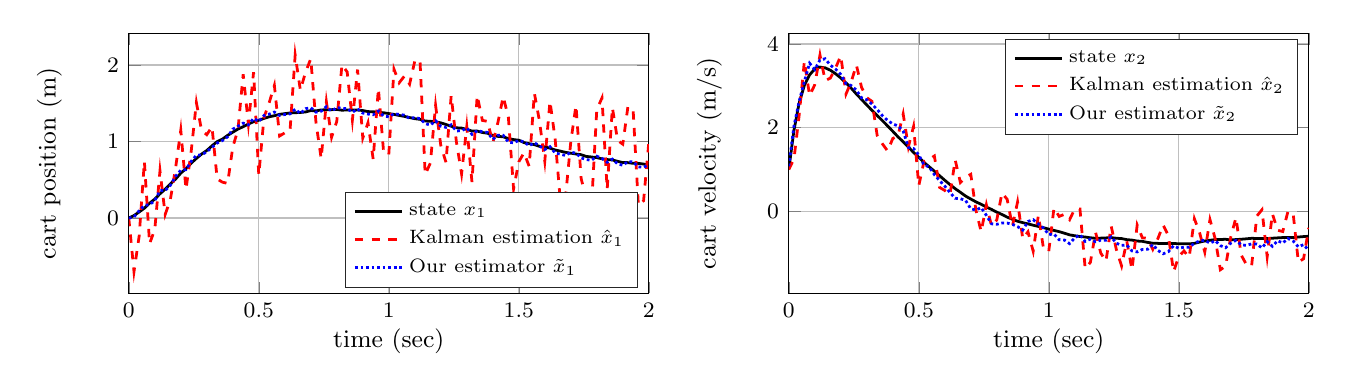
\begin{tikzpicture}
\begin{axis}
[	width=2.6in,
	height=1.3in,
	at={(0in,1.7in)},
	scale only axis,
	xmin=0,
	xmax=2.0,
	xlabel={\small time (sec)},
	ylabel={\small cart position (m)},
	x label style={at={(axis description cs:0.5,-0.1)},anchor=north},
	y label style={at={(axis description cs:-0.11,.5)},anchor=south},
	xticklabel style = {font=\footnotesize},
	yticklabel style = {font=\footnotesize},
	axis background/.style={fill=white},
	xmajorgrids,
	ymajorgrids,
	legend style={at={(0.98,0.02)}, anchor=south east, legend cell align=left, align=left, draw=white!15!black, font=\scriptsize}]
	 \addplot [color={black}, line width=1pt]
	table[row sep={\\}]
	{
0.0  0.0  \\
0.02  0.0312885282018752  \\
0.04  0.0788123875203588  \\
0.06  0.12783983276693056  \\
0.08  0.19302443002512482  \\
0.1  0.24691171369130704  \\
0.12  0.3161471924463811  \\
0.14  0.37655820357754827  \\
0.16  0.44574118653184464  \\
0.18  0.508717686134174  \\
0.2  0.5858944594685165  \\
0.22  0.6442080290694358  \\
0.24  0.7170003106288797  \\
0.26  0.7781390817476541  \\
0.28  0.8348607428170365  \\
0.3  0.8820850124163883  \\
0.32  0.9429843329186438  \\
0.34  0.9985281560618742  \\
0.36  1.0302635273555911  \\
0.38  1.0791321889652439  \\
0.4  1.121245022981027  \\
0.42  1.161891300602804  \\
0.44  1.192700117051156  \\
0.46  1.2287933108791957  \\
0.48  1.2579103583060975  \\
0.5  1.2769090558718827  \\
0.52  1.3010074939994656  \\
0.54  1.322606952127935  \\
0.56  1.3363739300408208  \\
0.58  1.3547060181087645  \\
0.6  1.3637156124358794  \\
0.62  1.372208147950066  \\
0.64  1.3758158415504202  \\
0.66  1.3789775570173455  \\
0.68  1.3858658992171147  \\
0.7  1.4038540774769968  \\
0.72  1.399388270372787  \\
0.74  1.4121158471937587  \\
0.76  1.413967536880243  \\
0.78  1.4159014376757404  \\
0.8  1.417828678620937  \\
0.82  1.408439121962671  \\
0.84  1.4119812043541529  \\
0.86  1.4115583441626582  \\
0.88  1.4107211138008886  \\
0.9  1.4043543531943106  \\
0.92  1.390269579268504  \\
0.94  1.388444098074998  \\
0.96  1.3811571553361286  \\
0.98  1.375136659753237  \\
1.0  1.3650405410205926  \\
1.02  1.3532746327113854  \\
1.04  1.3399687394128827  \\
1.06  1.3274222529638806  \\
1.08  1.312887237057181  \\
1.1  1.297953855938006  \\
1.12  1.2888243656725031  \\
1.14  1.2671580891040044  \\
1.16  1.2636596712198738  \\
1.18  1.2568123705161265  \\
1.2  1.2433534208208616  \\
1.22  1.222018058868546  \\
1.24  1.199082947901861  \\
1.26  1.1789132315105741  \\
1.28  1.1746923163614416  \\
1.3  1.1574829037716936  \\
1.32  1.1356654326585793  \\
1.34  1.1362230591177622  \\
1.36  1.1171876047888512  \\
1.38  1.1074990138885137  \\
1.4  1.078974551777622  \\
1.42  1.0661973181301283  \\
1.44  1.0609127088404313  \\
1.46  1.0372993334160026  \\
1.48  1.024440355201395  \\
1.5  1.016773165435164  \\
1.52  0.985372726177421  \\
1.54  0.9708403750356196  \\
1.56  0.9591509832628655  \\
1.58  0.9355856912687716  \\
1.6  0.9288408011304456  \\
1.62  0.9124527452153604  \\
1.64  0.888692309701688  \\
1.66  0.8736279796836832  \\
1.68  0.8576149131794482  \\
1.7  0.8467338065845937  \\
1.72  0.8357323419078908  \\
1.74  0.8271295129691318  \\
1.76  0.804168519172342  \\
1.78  0.7973787024419723  \\
1.8  0.7885831880803513  \\
1.82  0.7731913576797228  \\
1.84  0.7632841476573989  \\
1.86  0.7581919965043644  \\
1.88  0.7404424073275442  \\
1.9  0.7242330930938433  \\
1.92  0.7232652267292055  \\
1.94  0.7141451711559598  \\
1.96  0.7135626060421556  \\
1.98  0.7050839449630739  \\
2.0  0.6894219585423397  \\
	}
	;\addlegendentry{state $x_1$}
	
	\addplot [color={red},dashed, line width=1pt]
	table[row sep={\\}]
	{
 0.0  0.0  \\
0.02  -0.7016326820685982  \\
0.04  -0.23585571586261345  \\
0.06  0.7396609099297807  \\
0.08  -0.33621243440965815  \\
0.1  -0.15048791253219151  \\
0.12  0.6176826620511138  \\
0.14  0.04578213612712215  \\
0.16  0.24085153712000212  \\
0.18  0.6519749416537854  \\
0.2  1.1481340088757428  \\
0.22  0.3739654072288668  \\
0.24  0.8695195317551777  \\
0.26  1.5079986424406817  \\
0.28  1.1437489242746022  \\
0.3  1.0884297575593251  \\
0.32  1.192645206389877  \\
0.34  0.5096949773855692  \\
0.36  0.4682016134464051  \\
0.38  0.45158731684792996  \\
0.4  0.9245292733660191  \\
0.42  1.1563184823107087  \\
0.44  1.8782643853325425  \\
0.46  1.2286200415610418  \\
0.48  1.90560288844914  \\
0.5  0.5609048675886162  \\
0.52  1.314072432246385  \\
0.54  1.506294966924829  \\
0.56  1.732157136746129  \\
0.58  1.0713638460394828  \\
0.6  1.1124754014038012  \\
0.62  1.1325698189447386  \\
0.64  2.1299447613993494  \\
0.66  1.6694764974183034  \\
0.68  1.9074552913612985  \\
0.7  2.0802230570514464  \\
0.72  1.249075947340938  \\
0.74  0.7755524566336746  \\
0.76  1.5186582695973136  \\
0.78  1.053934096560571  \\
0.8  1.263845037327248  \\
0.82  2.004341804511319  \\
0.84  1.9076177543863433  \\
0.86  1.2791803217886837  \\
0.88  1.9388924541370987  \\
0.9  1.044856742034207  \\
0.92  1.2434718255294455  \\
0.94  0.7678933158489609  \\
0.96  1.6943045521016002  \\
0.98  0.8649726988503483  \\
1.0  0.826956736056349  \\
1.02  1.9441067890112704  \\
1.04  1.7671483990223398  \\
1.06  1.8537757329684719  \\
1.08  1.74869596272442  \\
1.1  2.050331385127062  \\
1.12  2.065323459242827  \\
1.14  0.5675645417737036  \\
1.16  0.7183137980272856  \\
1.18  1.4721749444770658  \\
1.2  0.9486696263681218  \\
1.22  0.7275878036994118  \\
1.24  1.5982571538598647  \\
1.26  0.9968108122528502  \\
1.28  0.5771790217717717  \\
1.3  1.1939220530371921  \\
1.32  0.4705513491038608  \\
1.34  1.6017654267607948  \\
1.36  1.2754776607476657  \\
1.38  1.2618686905389338  \\
1.4  0.9821092898946824  \\
1.42  1.2520370722954877  \\
1.44  1.5868463335267238  \\
1.46  1.315316213744334  \\
1.48  0.3809467176356255  \\
1.5  0.7343497684517054  \\
1.52  0.8525011066231617  \\
1.54  0.6747786775563649  \\
1.56  1.631306074588672  \\
1.58  1.259238093266994  \\
1.6  0.7406502576917274  \\
1.62  1.5270858735962223  \\
1.64  1.0273604220689518  \\
1.66  0.22013248694006454  \\
1.68  0.2814102904932267  \\
1.7  0.9937623709318437  \\
1.72  1.4722659204159319  \\
1.74  0.513230720725658  \\
1.76  0.24399096723995706  \\
1.78  0.17209686923052656  \\
1.8  1.414894962085707  \\
1.82  1.5689427180553022  \\
1.84  0.3738299073894682  \\
1.86  1.4432830585706296  \\
1.88  1.0146304626081781  \\
1.9  0.9646143450049791  \\
1.92  1.4599263074280486  \\
1.94  1.3992941378715475  \\
1.96  0.16577497949085318  \\
1.98  0.2250988953546872  \\
2.0  0.9813678260080361  \\
	}
	;\addlegendentry{{ Kalman estimation $\hat{x}_1$}}
    \addplot[densely dotted, color={blue}, line width=1pt]
        table[row sep={\\}]
        {
  0.0  -0.0016546478915138397  \\
0.02  0.012803800843751626  \\
0.04  0.09554688470489497  \\
0.06  0.16253616814154492  \\
0.08  0.1757155439630189  \\
0.1  0.22684144474391166  \\
0.12  0.3588610317373191  \\
0.14  0.3600565285670698  \\
0.16  0.4268314405275966  \\
0.18  0.5444687411092691  \\
0.2  0.6240844791843322  \\
0.22  0.6314795408897524  \\
0.24  0.7400311038559425  \\
0.26  0.8189832083536872  \\
0.28  0.8244024397244267  \\
0.3  0.8663905052304092  \\
0.32  0.922990301770209  \\
0.34  0.9798892619734936  \\
0.36  1.0117967230429303  \\
0.38  1.0599172908675325  \\
0.4  1.1603643852567949  \\
0.42  1.1990802015445396  \\
0.44  1.2395813207698205  \\
0.46  1.2165585171583397  \\
0.48  1.3013264919921557  \\
0.5  1.2609307571835484  \\
0.52  1.3386884784369582  \\
0.54  1.357083577925525  \\
0.56  1.3842326654411976  \\
0.58  1.3398267024517447  \\
0.6  1.3518845191939897  \\
0.62  1.3605004189076775  \\
0.64  1.4219380480003003  \\
0.66  1.3649203285273799  \\
0.68  1.4285890406210218  \\
0.7  1.4410836824050024  \\
0.72  1.3826840414912316  \\
0.74  1.3959236008102323  \\
0.76  1.4552823453620856  \\
0.78  1.3959039513270748  \\
0.8  1.4438071511837156  \\
0.82  1.432844078488602  \\
0.84  1.4299867320429205  \\
0.86  1.3813759762529558  \\
0.88  1.4265818351347233  \\
0.9  1.3709250480900586  \\
0.92  1.3579677545976403  \\
0.94  1.3487742263587437  \\
0.96  1.3975588490058366  \\
0.98  1.33454216140927  \\
1.0  1.3216205976334596  \\
1.02  1.3624960268492265  \\
1.04  1.353311126347017  \\
1.06  1.3439501738480442  \\
1.08  1.301369848305021  \\
1.1  1.3125870668179422  \\
1.12  1.2980724796332295  \\
1.14  1.2338677686687103  \\
1.16  1.2137553744273737  \\
1.18  1.2709021953976292  \\
1.2  1.1992025218793143  \\
1.22  1.183697398088326  \\
1.24  1.218570516572107  \\
1.26  1.137563007619231  \\
1.28  1.1405022675978889  \\
1.3  1.1765535132579692  \\
1.32  1.0928758663920797  \\
1.34  1.1414652285997844  \\
1.36  1.1271940964802922  \\
1.38  1.1178376669643972  \\
1.4  1.0277986083364172  \\
1.42  1.0805816091531892  \\
1.44  1.0807849167204544  \\
1.46  0.9920763178114405  \\
1.48  0.9817306703518764  \\
1.5  1.0134477693156418  \\
1.52  0.9951974251474277  \\
1.54  0.9442285914088713  \\
1.56  0.9833197436088972  \\
1.58  0.9409151710618642  \\
1.6  0.8946300833123895  \\
1.62  0.9316112622492073  \\
1.64  0.8489701821077618  \\
1.66  0.8339106994871763  \\
1.68  0.8161789446932478  \\
1.7  0.859266662119662  \\
1.72  0.8476876655078228  \\
1.74  0.7855933449829767  \\
1.76  0.7624117087703305  \\
1.78  0.7551194589099179  \\
1.8  0.8077894968082772  \\
1.82  0.7782348664563057  \\
1.84  0.7291031405864548  \\
1.86  0.7692963458943343  \\
1.88  0.7074919875254148  \\
1.9  0.6891930843264874  \\
1.92  0.7372792789114803  \\
1.94  0.7335083478070233  \\
1.96  0.668317016120237  \\
1.98  0.6637710011872  \\
2.0  0.6980071501144504  \\
        }
        ;\addlegendentry{{ Our estimator $\tilde{x}_1$}}
        
\end{axis}

\begin{axis}
[	width=2.6in,
height=1.3in,
at={(3.3in,1.7in)},
scale only axis,
xmin=0,
xmax=2.0,
xlabel={\small time (sec)},
ylabel={\small cart velocity (m/s)},
x label style={at={(axis description cs:0.5,-0.1)},anchor=north},
y label style={at={(axis description cs:-0.11,.5)},anchor=south},
xticklabel style = {font=\footnotesize},
yticklabel style = {font=\footnotesize},
axis background/.style={fill=white},
xmajorgrids,
ymajorgrids,
legend style={at={(0.98,0.98)}, anchor=north east, legend cell align=left, align=left, draw=white!15!black, font=\scriptsize}]
\addplot [color={black}, line width=1pt]
table[row sep={\\}]
{
0.0  1.0  \\
0.02  1.9391209237895848  \\
0.04  2.590989465213296  \\
0.06  3.0112038136322097  \\
0.08  3.262145933341507  \\
0.1  3.404055223712122  \\
0.12  3.448329465319425  \\
0.14  3.4304868325634814  \\
0.16  3.372844199991032  \\
0.18  3.289148790648013  \\
0.2  3.1885535486300065  \\
0.22  3.0692926604120068  \\
0.24  2.944939735179303  \\
0.26  2.8041012335303797  \\
0.28  2.6741250131880947  \\
0.3  2.542186317426113  \\
0.32  2.4133137843864088  \\
0.34  2.2902036362827154  \\
0.36  2.1676068541377513  \\
0.38  2.041575453393154  \\
0.4  1.912003547154351  \\
0.42  1.7805111075137916  \\
0.44  1.6613280032011057  \\
0.46  1.5367336043391617  \\
0.48  1.4056656658012763  \\
0.5  1.290973151946963  \\
0.52  1.1679927469559728  \\
0.54  1.0638319121527307  \\
0.56  0.9574423074532515  \\
0.58  0.8490799761838703  \\
0.6  0.7412336946439754  \\
0.62  0.6375781972725671  \\
0.64  0.5397855090185257  \\
0.66  0.4532142587467182  \\
0.68  0.36280368622739734  \\
0.7  0.2917937269950741  \\
0.72  0.22364279659665026  \\
0.74  0.16641956056250445  \\
0.76  0.09957734983786248  \\
0.78  0.04285943612658093  \\
0.8  -0.021996866697433476  \\
0.82  -0.07785062469992182  \\
0.84  -0.14179940204160668  \\
0.86  -0.192111834507433  \\
0.88  -0.2395799342971533  \\
0.9  -0.2731098299450826  \\
0.92  -0.3023493674467045  \\
0.94  -0.33494599088485866  \\
0.96  -0.3634837919419665  \\
0.98  -0.39429252436904916  \\
1.0  -0.427376069393288  \\
1.02  -0.45849247351460987  \\
1.04  -0.4886944820743368  \\
1.06  -0.5253851993311534  \\
1.08  -0.5650389302187308  \\
1.1  -0.5863884385696589  \\
1.12  -0.6038458947549443  \\
1.14  -0.6171167795918366  \\
1.16  -0.6349431570995152  \\
1.18  -0.6474517267585185  \\
1.2  -0.6434772685824866  \\
1.22  -0.6379941265376432  \\
1.24  -0.6322982024232  \\
1.26  -0.6458598128233805  \\
1.28  -0.654065958989119  \\
1.3  -0.679509056048515  \\
1.32  -0.6905768067028223  \\
1.34  -0.7130004889104322  \\
1.36  -0.7203615215047533  \\
1.38  -0.7454102026881453  \\
1.4  -0.7645886120566366  \\
1.42  -0.7688770436773459  \\
1.44  -0.7733996969520899  \\
1.46  -0.767714095270773  \\
1.48  -0.7704943594144114  \\
1.5  -0.7792436303557043  \\
1.52  -0.7763125311369948  \\
1.54  -0.7800818638691298  \\
1.56  -0.7683618200545922  \\
1.58  -0.7379645382430333  \\
1.6  -0.7120211968404369  \\
1.62  -0.6944313784107807  \\
1.64  -0.6788356905664363  \\
1.66  -0.6755209780869861  \\
1.68  -0.6713863855448137  \\
1.7  -0.6861143109771883  \\
1.72  -0.6777605242430396  \\
1.74  -0.67008745456601  \\
1.76  -0.6595296803854034  \\
1.78  -0.6480090140165278  \\
1.8  -0.651450136105128  \\
1.82  -0.6517143018493359  \\
1.84  -0.6525749963680775  \\
1.86  -0.6453041999310413  \\
1.88  -0.6373422062650471  \\
1.9  -0.630057062238385  \\
1.92  -0.6301433102561566  \\
1.94  -0.6297353309511714  \\
1.96  -0.616497720752044  \\
1.98  -0.6064299270620612  \\
2.0  -0.5981417131472986  \\
}
;\addlegendentry{state $x_2$}

\addplot [color={red},dashed, line width=1pt]
table[row sep={\\}]
{
   0.0  1.0  \\
0.02  1.2520375776998334  \\
0.04  2.300009604013391  \\
0.06  3.592060558953479  \\
0.08  2.7649250252416024  \\
0.1  3.0262809894865192  \\
0.12  3.737499294098212  \\
0.14  3.12110372825729  \\
0.16  3.1861891324106963  \\
0.18  3.4274138963467804  \\
0.2  3.7198764070873898  \\
0.22  2.803236665480386  \\
0.24  3.0913857467081614  \\
0.26  3.500316410919404  \\
0.28  2.961819884446753  \\
0.3  2.7158798761007077  \\
0.32  2.628985356939085  \\
0.34  1.812881338210877  \\
0.36  1.613351795096433  \\
0.38  1.4425020734693912  \\
0.4  1.7399265201110468  \\
0.42  1.8028149398680218  \\
0.44  2.326401112633281  \\
0.46  1.5423332185675656  \\
0.48  2.0287784649248946  \\
0.5  0.6102389896017371  \\
0.52  1.191268735603829  \\
0.54  1.237764042431899  \\
0.56  1.3224531999777234  \\
0.58  0.5704468281498346  \\
0.6  0.49673279383399516  \\
0.62  0.3981857887619049  \\
0.64  1.229096741477517  \\
0.66  0.6877935606365496  \\
0.68  0.8141279419565274  \\
0.7  0.8835958773833297  \\
0.72  0.020568475438498934  \\
0.74  -0.48943871844095244  \\
0.76  0.15514500137660914  \\
0.78  -0.35244027450211646  \\
0.8  -0.20815875770989178  \\
0.82  0.438027801028096  \\
0.84  0.2843113304577627  \\
0.86  -0.36055354865939027  \\
0.88  0.22295697043163942  \\
0.9  -0.6589673240118565  \\
0.92  -0.49078963983506707  \\
0.94  -0.9568518427371487  \\
0.96  -0.09412376172945769  \\
0.98  -0.9039459953155622  \\
1.0  -0.9563233110889232  \\
1.02  0.07966430313712625  \\
1.04  -0.12380509206160606  \\
1.06  -0.07402619999655324  \\
1.08  -0.2030130407085846  \\
1.1  0.056772989288457865  \\
1.12  0.052243394850999936  \\
1.14  -1.3723270099750198  \\
1.16  -1.223561027584351  \\
1.18  -0.5057712567390962  \\
1.2  -1.0011869394094126  \\
1.22  -1.1949065410616595  \\
1.24  -0.3549026777961153  \\
1.26  -0.9183435604352458  \\
1.28  -1.3080548317301632  \\
1.3  -0.7141746173316741  \\
1.32  -1.40188819595665  \\
1.34  -0.32959480344887826  \\
1.36  -0.6367413723090429  \\
1.38  -0.6468663524250073  \\
1.4  -0.9123046246791389  \\
1.42  -0.6493285146517109  \\
1.44  -0.3288712775744558  \\
1.46  -0.5838383248759282  \\
1.48  -1.4457255354947045  \\
1.5  -1.081487548739723  \\
1.52  -0.9510426624820778  \\
1.54  -1.1035250307171802  \\
1.56  -0.17920451360073142  \\
1.58  -0.5104956175392936  \\
1.6  -0.9774753425770938  \\
1.62  -0.20198433902106339  \\
1.64  -0.6568916513437502  \\
1.66  -1.400750886670715  \\
1.68  -1.3131253278757518  \\
1.7  -0.615670432340711  \\
1.72  -0.15068321641309024  \\
1.74  -1.046636962700916  \\
1.76  -1.2754309384409042  \\
1.78  -1.3185154829093082  \\
1.8  -0.11618707527794592  \\
1.82  0.03486447792739433  \\
1.84  -1.0885087582132544  \\
1.86  -0.05963010563322024  \\
1.88  -0.4554360354252778  \\
1.9  -0.48533050983918957  \\
1.92  -0.004104539990258171  \\
1.94  -0.05907869157379575  \\
1.96  -1.2193817306049763  \\
1.98  -1.1368577322583464  \\
2.0  -0.39764266241265944  \\
}
;\addlegendentry{{ Kalman estimation $\hat{x}_2$}}
\addplot[densely dotted, color={blue}, line width=1pt]
table[row sep={\\}]
{
 0.0  1.0766943557990734  \\
0.02  2.0402360299618394  \\
0.04  2.6309454758292494  \\
0.06  3.1068675196902764  \\
0.08  3.54080134552669  \\
0.1  3.390423831584909  \\
0.12  3.6176773435075993  \\
0.14  3.6483302835825806  \\
0.16  3.4940837403221066  \\
0.18  3.400518174132703  \\
0.2  3.272179041445286  \\
0.22  3.051182580312056  \\
0.24  3.007136640276949  \\
0.26  2.89668735820574  \\
0.28  2.713233393415006  \\
0.3  2.666081620611238  \\
0.32  2.562083551484879  \\
0.34  2.434075387513464  \\
0.36  2.286871848307895  \\
0.38  2.1725112918581857  \\
0.4  2.0891911107037067  \\
0.42  2.0406855463131692  \\
0.44  1.9222977654197195  \\
0.46  1.5257739757194784  \\
0.48  1.4989888926426562  \\
0.5  1.3473304530955497  \\
0.52  1.109572133570126  \\
0.54  1.0592201977960447  \\
0.56  0.8758454837144379  \\
0.58  0.7337559238480325  \\
0.6  0.6004573856743581  \\
0.62  0.44824465603343244  \\
0.64  0.3101689801671155  \\
0.66  0.2987946638154928  \\
0.68  0.2600433017728896  \\
0.7  0.05672463712827543  \\
0.72  0.030413094277216744  \\
0.74  0.08555028416184272  \\
0.76  -0.09971583953501285  \\
0.78  -0.3017142438245463  \\
0.8  -0.3122042796770449  \\
0.82  -0.2827534315188673  \\
0.84  -0.2829505347667381  \\
0.86  -0.31444525280989494  \\
0.88  -0.3679083896574561  \\
0.9  -0.4523096410930004  \\
0.92  -0.24528076875533894  \\
0.94  -0.2012204257573242  \\
0.96  -0.30459353150941115  \\
0.98  -0.4034606060932498  \\
1.0  -0.5579468081734421  \\
1.02  -0.5456885041145905  \\
1.04  -0.6834788869342028  \\
1.06  -0.6876029558751029  \\
1.08  -0.7754242277751354  \\
1.1  -0.6357568393571198  \\
1.12  -0.5647630895137999  \\
1.14  -0.722224950479285  \\
1.16  -0.6672023210232  \\
1.18  -0.730160044324085  \\
1.2  -0.6932767721446531  \\
1.22  -0.6955416637290003  \\
1.24  -0.6148744413228993  \\
1.26  -0.7646738905171426  \\
1.28  -0.8174879195874942  \\
1.3  -0.8086440314412106  \\
1.32  -0.9489524673668117  \\
1.34  -0.9731834368682155  \\
1.36  -0.9134270631253525  \\
1.38  -0.9095082237264895  \\
1.4  -0.7968292615369957  \\
1.42  -0.9388984989978707  \\
1.44  -1.0175358467975835  \\
1.46  -0.9680022103203125  \\
1.48  -0.8260065615129651  \\
1.5  -0.886260333768104  \\
1.52  -0.8603670806734103  \\
1.54  -0.8640190493688218  \\
1.56  -0.7640364116753472  \\
1.58  -0.7120111509452782  \\
1.6  -0.6936300126424111  \\
1.62  -0.764741414382075  \\
1.64  -0.7033854196176764  \\
1.66  -0.8226871876980503  \\
1.68  -0.8731757555208807  \\
1.7  -0.7626857480875107  \\
1.72  -0.6967479415177407  \\
1.74  -0.8031387793448946  \\
1.76  -0.8170700823758712  \\
1.78  -0.7816777307010934  \\
1.8  -0.7845261659077962  \\
1.82  -0.8770371475311388  \\
1.84  -0.7264585052225073  \\
1.86  -0.8394900475907195  \\
1.88  -0.705278834141262  \\
1.9  -0.760571799602993  \\
1.92  -0.650966035713089  \\
1.94  -0.7135157071013508  \\
1.96  -0.8527263663135067  \\
1.98  -0.7989930114769055  \\
2.0  -0.9373767100494399  \\
}
;\addlegendentry{{ Our estimator $\tilde{x}_2$}}

\end{axis}

%  	\begin{axis}
%	[	width=2.6in,
%	height=1.3in,
%	at={(0in,0in)},
%	scale only axis,
%	xmin=0,
%	xmax=2.0,
%%	ymin=-4,
%%	ymax=2,
%	xlabel={\small time (sec)},
%	ylabel={\small $x_3$ pendulumn angle},
%	x label style={at={(axis description cs:0.5,-0.1)},anchor=north},
%	y label style={at={(axis description cs:-0.11,.5)},anchor=south},
%	xticklabel style = {font=\footnotesize},
%	yticklabel style = {font=\footnotesize},
%	axis background/.style={fill=white},
%	xmajorgrids,
%	ymajorgrids,
%	legend style={at={(0.98,0.02)}, anchor=south east, legend cell align=left, align=left, draw=white!15!black, font=\scriptsize}]
%	\addplot [color={black}, line width=1pt]
%	table[row sep={\\}]
%	{
%0.0  0.0  \\
%0.02  0.00772853593415913  \\
%0.04  0.004801671416923327  \\
%0.06  -0.012528997431996048  \\
%0.08  -0.034478619332425936  \\
%0.1  -0.06220231524500317  \\
%0.12  -0.08812635048651297  \\
%0.14  -0.11408845091735348  \\
%0.16  -0.14488997218330013  \\
%0.18  -0.16947348245078697  \\
%0.2  -0.19501471373927462  \\
%0.22  -0.2166030568036244  \\
%0.24  -0.23694887645664164  \\
%0.26  -0.2534179553657174  \\
%0.28  -0.2659048131170473  \\
%0.3  -0.2814074322954603  \\
%0.32  -0.2947651384686937  \\
%0.34  -0.30280625979339526  \\
%0.36  -0.3110461733895194  \\
%0.38  -0.322599925444607  \\
%0.4  -0.3266601375700984  \\
%0.42  -0.32832183302190043  \\
%0.44  -0.33079378651792585  \\
%0.46  -0.33139999061403563  \\
%0.48  -0.33190912976035625  \\
%0.5  -0.32830514918189446  \\
%0.52  -0.3265624628054656  \\
%0.54  -0.3231032971609128  \\
%0.56  -0.31943423376946206  \\
%0.58  -0.31567219360956844  \\
%0.6  -0.3139459878003922  \\
%0.62  -0.30858429971742735  \\
%0.64  -0.302866065490615  \\
%0.66  -0.2975240107704187  \\
%0.68  -0.29156813130488785  \\
%0.7  -0.28705864201984305  \\
%0.72  -0.2800613967051828  \\
%0.74  -0.2721345042496352  \\
%0.76  -0.2675647476463787  \\
%0.78  -0.26004373544306775  \\
%0.8  -0.24895562242482422  \\
%0.82  -0.24469615255703123  \\
%0.84  -0.23679296240647962  \\
%0.86  -0.22526462977535064  \\
%0.88  -0.21530137387528134  \\
%0.9  -0.2019610820610649  \\
%0.92  -0.19283115640996426  \\
%0.94  -0.18404650174938508  \\
%0.96  -0.1761938176509628  \\
%0.98  -0.16952154188571567  \\
%1.0  -0.16068318494400077  \\
%1.02  -0.15115385465801076  \\
%1.04  -0.142077499764086  \\
%1.06  -0.13285231555738442  \\
%1.08  -0.12217488148841449  \\
%1.1  -0.11717625074624005  \\
%1.12  -0.11014342489808715  \\
%1.14  -0.10290962697247244  \\
%1.16  -0.09707223606283309  \\
%1.18  -0.08535583686102192  \\
%1.2  -0.07985586728850495  \\
%1.22  -0.07053290137389215  \\
%1.24  -0.0660756875734225  \\
%1.26  -0.05925950423578198  \\
%1.28  -0.04983238664926049  \\
%1.3  -0.046321730532286276  \\
%1.32  -0.04111947230774583  \\
%1.34  -0.03716014124124552  \\
%1.36  -0.026958173254637667  \\
%1.38  -0.02105479624823502  \\
%1.4  -0.013204082238369545  \\
%1.42  -0.007208612852129617  \\
%1.44  -0.005029793064317797  \\
%1.46  -0.0030365387904538444  \\
%1.48  -0.004685191023569348  \\
%1.5  -0.0013502134977833556  \\
%1.52  -0.0012637857934116841  \\
%1.54  -0.0012840803221537893  \\
%1.56  0.004161592495718868  \\
%1.58  0.007337270321035059  \\
%1.6  0.007873265952081725  \\
%1.62  0.007756595504494869  \\
%1.64  0.012948213825993315  \\
%1.66  0.01713997304166258  \\
%1.68  0.019303428528959714  \\
%1.7  0.021720664071569973  \\
%1.72  0.021496525088056485  \\
%1.74  0.02269954427453162  \\
%1.76  0.025127263635035712  \\
%1.78  0.025581388241573386  \\
%1.8  0.022956371536018347  \\
%1.82  0.020320909246699284  \\
%1.84  0.02325727363447171  \\
%1.86  0.022566429135964905  \\
%1.88  0.025410932971556357  \\
%1.9  0.025581397517493814  \\
%1.92  0.024133015365711413  \\
%1.94  0.024607306183292644  \\
%1.96  0.02686997993370564  \\
%1.98  0.028618584557972122  \\
%2.0  0.02949612536857937  \\
%	}
%	;\addlegendentry{state $x_3$}
%	\addplot [color={red},dashed, line width=1pt]
%	table[row sep={\\}]
%	{
%	 0.0  0.0  \\
%	0.02  0.00809402453328914  \\
%	0.04  0.002283710058266839  \\
%	0.06  -0.011924222353404363  \\
%	0.08  -0.03538807548199385  \\
%	0.1  -0.062495688561897404  \\
%	0.12  -0.08979727756857352  \\
%	0.14  -0.11596912737252132  \\
%	0.16  -0.14427298978459968  \\
%	0.18  -0.1699091880689923  \\
%	0.2  -0.19571409358693093  \\
%	0.22  -0.21710723871475957  \\
%	0.24  -0.23750518798723996  \\
%	0.26  -0.2523487237267693  \\
%	0.28  -0.26564551359739796  \\
%	0.3  -0.28113924184632594  \\
%	0.32  -0.29344313265186917  \\
%	0.34  -0.30387742299429843  \\
%	0.36  -0.31093266172634626  \\
%	0.38  -0.32032314034771303  \\
%	0.4  -0.32488432492231156  \\
%	0.42  -0.328256133800731  \\
%	0.44  -0.33170684466667966  \\
%	0.46  -0.33284554813223155  \\
%	0.48  -0.32934060251669267  \\
%	0.5  -0.32881415681358606  \\
%	0.52  -0.32672393145274836  \\
%	0.54  -0.3217023284966502  \\
%	0.56  -0.31920782046530927  \\
%	0.58  -0.3155857583713461  \\
%	0.6  -0.31200171978648444  \\
%	0.62  -0.30753884981430435  \\
%	0.64  -0.30328744734313084  \\
%	0.66  -0.298819639225292  \\
%	0.68  -0.2916263924411364  \\
%	0.7  -0.2838538399639527  \\
%	0.72  -0.27822533107121034  \\
%	0.74  -0.27214850374295424  \\
%	0.76  -0.2649862125224101  \\
%	0.78  -0.2581935349054245  \\
%	0.8  -0.24687375692743166  \\
%	0.82  -0.24215334598492766  \\
%	0.84  -0.23463968652823464  \\
%	0.86  -0.2266454648618093  \\
%	0.88  -0.21570653361944153  \\
%	0.9  -0.20378113555698663  \\
%	0.92  -0.1922094272504351  \\
%	0.94  -0.18193892229656553  \\
%	0.96  -0.17462306148804935  \\
%	0.98  -0.16857998362472904  \\
%	1.0  -0.1589098101915298  \\
%	1.02  -0.1502282447377052  \\
%	1.04  -0.14310208638808308  \\
%	1.06  -0.13391428982914821  \\
%	1.08  -0.12206666034954945  \\
%	1.1  -0.11753381580332939  \\
%	1.12  -0.11064111898353321  \\
%	1.14  -0.10215982660161821  \\
%	1.16  -0.096618902112179  \\
%	1.18  -0.08817640412095815  \\
%	1.2  -0.07931844432254224  \\
%	1.22  -0.0713170158403937  \\
%	1.24  -0.06598326032462205  \\
%	1.26  -0.05869782541506201  \\
%	1.28  -0.05244831403760163  \\
%	1.3  -0.04689123976106053  \\
%	1.32  -0.04325454089798624  \\
%	1.34  -0.03885220256504527  \\
%	1.36  -0.030517495413270805  \\
%	1.38  -0.024466342268987945  \\
%	1.4  -0.018729185184462  \\
%	1.42  -0.010157661361933055  \\
%	1.44  -0.005799650225733364  \\
%	1.46  -0.0017710381011364653  \\
%	1.48  -0.002224799382994183  \\
%	1.5  -0.0037629560253844437  \\
%	1.52  -0.00020440203585928116  \\
%	1.54  0.0012643359647233753  \\
%	1.56  0.003252784378121404  \\
%	1.58  0.005266412443152401  \\
%	1.6  0.006949937595322902  \\
%	1.62  0.008256452575278935  \\
%	1.64  0.012007453507124496  \\
%	1.66  0.01615310418726861  \\
%	1.68  0.019000666804788804  \\
%	1.7  0.022087371511188413  \\
%	1.72  0.022261092399250972  \\
%	1.74  0.02355749395802008  \\
%	1.76  0.023895346270558754  \\
%	1.78  0.026333022304786253  \\
%	1.8  0.02456626556539792  \\
%	1.82  0.021605386228436392  \\
%	1.84  0.023528349423668403  \\
%	1.86  0.023572743261476937  \\
%	1.88  0.025126899283551846  \\
%	1.9  0.025833933274513415  \\
%	1.92  0.02280935517999988  \\
%	1.94  0.025189469054832925  \\
%	1.96  0.02661138935665535  \\
%	1.98  0.02763011362829756  \\
%	2.0  0.027469141828147026  \\
%	}
%	;\addlegendentry{{ Kalman estimation $\hat{x}_3$}}
%	\addplot[densely dotted, color={blue}, line width=1pt]
%	table[row sep={\\}]
%	{
%    0.0  1.8153964737662312e-5  \\
%0.02  0.0066894619554046355  \\
%0.04  0.0018375871994040162  \\
%0.06  -0.011012697570773474  \\
%0.08  -0.03609804873935931  \\
%0.1  -0.06340645502442915  \\
%0.12  -0.0895457918792631  \\
%0.14  -0.11546107462068377  \\
%0.16  -0.14461477831571443  \\
%0.18  -0.17007154514361927  \\
%0.2  -0.1965051643232883  \\
%0.22  -0.2166340902306285  \\
%0.24  -0.23770039325448397  \\
%0.26  -0.2507335125541037  \\
%0.28  -0.2645156857629006  \\
%0.3  -0.28216527675191616  \\
%0.32  -0.2939902057265568  \\
%0.34  -0.30440857374041375  \\
%0.36  -0.31047444062583235  \\
%0.38  -0.32198495278139255  \\
%0.4  -0.3249118700086211  \\
%0.42  -0.32841640163734204  \\
%0.44  -0.33251010788936297  \\
%0.46  -0.3331188005365526  \\
%0.48  -0.32767165979082796  \\
%0.5  -0.3288637216034393  \\
%0.52  -0.3265504673964966  \\
%0.54  -0.3205275268798475  \\
%0.56  -0.3197884422608594  \\
%0.58  -0.3157679939079811  \\
%0.6  -0.31254421435944685  \\
%0.62  -0.30806083114358135  \\
%0.64  -0.3038352148338218  \\
%0.66  -0.2994116819525727  \\
%0.68  -0.29121889287466646  \\
%0.7  -0.2833617882231757  \\
%0.72  -0.27936861590095097  \\
%0.74  -0.27290542088826425  \\
%0.76  -0.2654318394097727  \\
%0.78  -0.25942935600796185  \\
%0.8  -0.2457658293296008  \\
%0.82  -0.24403414344605018  \\
%0.84  -0.2358616914531913  \\
%0.86  -0.2275077308550984  \\
%0.88  -0.21485981313066116  \\
%0.9  -0.20232178782749977  \\
%0.92  -0.19104608352709898  \\
%0.94  -0.18111885006671183  \\
%0.96  -0.1754534261052666  \\
%0.98  -0.17003134488456753  \\
%1.0  -0.15878283143959224  \\
%1.02  -0.15051065091807594  \\
%1.04  -0.1435009071579159  \\
%1.06  -0.13363074186982313  \\
%1.08  -0.12038778178826819  \\
%1.1  -0.11866338138681089  \\
%1.12  -0.110930248968576  \\
%1.14  -0.10181163345285733  \\
%1.16  -0.09751700179946482  \\
%1.18  -0.08758702035485068  \\
%1.2  -0.07785509840417323  \\
%1.22  -0.07050311362538186  \\
%1.24  -0.06601841440192815  \\
%1.26  -0.05793710743206526  \\
%1.28  -0.051999353311811235  \\
%1.3  -0.04693730475850037  \\
%1.32  -0.04389217870983184  \\
%1.34  -0.038972560152190514  \\
%1.36  -0.02865888152011623  \\
%1.38  -0.02353592133370778  \\
%1.4  -0.017640744192343967  \\
%1.42  -0.007667707763960579  \\
%1.44  -0.004952961222438092  \\
%1.46  -0.0008037137317556581  \\
%1.48  -0.003445327891030425  \\
%1.5  -0.005518722706033974  \\
%1.52  0.0004546477429451413  \\
%1.54  0.0010515168391628813  \\
%1.56  0.0032978681139044274  \\
%1.58  0.005456467908684386  \\
%1.6  0.007016058115342972  \\
%1.62  0.007992613905111441  \\
%1.64  0.013215471326015648  \\
%1.66  0.01730891328170967  \\
%1.68  0.01980891940823777  \\
%1.7  0.023250483613783467  \\
%1.72  0.02194819975361911  \\
%1.74  0.023940958356646756  \\
%1.76  0.023721571245686246  \\
%1.78  0.027350023652804832  \\
%1.8  0.023546924861985615  \\
%1.82  0.019857344070720775  \\
%1.84  0.023909886569047793  \\
%1.86  0.0231294380862511  \\
%1.88  0.02574352864188202  \\
%1.9  0.025842587721728108  \\
%1.92  0.02092146538831675  \\
%1.94  0.025931184643444655  \\
%1.96  0.027084411024922466  \\
%1.98  0.027575839585923738  \\
%2.0  0.026971498895954696  \\
%	}
%;\addlegendentry{{our estimation $\tilde{x}_3$}}
%
%
%\end{axis}
%
%\begin{axis}
%[	width=2.6in,
%height=1.3in,
%at={(3.3in,0in)},
%scale only axis,
%xmin=0,
%xmax=2.0,
%%ymin=-4,
%%ymax=2,
%xlabel={\small time (sec)},
%ylabel={\small $x_4$ pendulumn angle velocity},
%x label style={at={(axis description cs:0.5,-0.1)},anchor=north},
%y label style={at={(axis description cs:-0.11,.5)},anchor=south},
%xticklabel style = {font=\footnotesize},
%yticklabel style = {font=\footnotesize},
%axis background/.style={fill=white},
%xmajorgrids,
%ymajorgrids,
%legend style={at={(0.98,0.02)}, anchor=south east, legend cell align=left, align=left, draw=white!15!black, font=\scriptsize}]
%\addplot [color={black}, line width=1pt]
%table[row sep={\\}]
%{
%  0.0  1.0  \\
%0.02  0.05313305390126177  \\
%0.04  -0.5807597079886778  \\
%0.06  -0.9849649892184913  \\
%0.08  -1.2236616544745775  \\
%0.1  -1.3448708265564777  \\
%0.12  -1.3911973425235322  \\
%0.14  -1.3847017109780744  \\
%0.16  -1.3360588370385862  \\
%0.18  -1.2612956960549269  \\
%0.2  -1.1712121233640451  \\
%0.22  -1.071999578445813  \\
%0.24  -0.9674797110228057  \\
%0.26  -0.8680549183886634  \\
%0.28  -0.7699884280336178  \\
%0.3  -0.6746842796248621  \\
%0.32  -0.586875654761506  \\
%0.34  -0.4959299174041296  \\
%0.36  -0.40597661697079446  \\
%0.38  -0.32771095994654365  \\
%0.4  -0.253961547290701  \\
%0.42  -0.18263871652089975  \\
%0.44  -0.11573407741218594  \\
%0.46  -0.05911515161120641  \\
%0.48  0.0009801138197992887  \\
%0.5  0.04463813200237973  \\
%0.52  0.09038368590143643  \\
%0.54  0.12381466371390598  \\
%0.56  0.16193471899976158  \\
%0.58  0.19217803962499197  \\
%0.6  0.2284585486584002  \\
%0.62  0.27315223526991256  \\
%0.64  0.3029744279918313  \\
%0.66  0.3360381761463694  \\
%0.68  0.36405311581028843  \\
%0.7  0.3862145241118462  \\
%0.72  0.4052381391063923  \\
%0.74  0.40659407112164414  \\
%0.76  0.4016463115722345  \\
%0.78  0.39680426743202124  \\
%0.8  0.3921338510569967  \\
%0.82  0.3884591608505884  \\
%0.84  0.3897778445333768  \\
%0.86  0.3978434385510643  \\
%0.88  0.40888248291393214  \\
%0.9  0.40349125898703586  \\
%0.92  0.4043181979298124  \\
%0.94  0.4001713487291486  \\
%0.96  0.397537790317619  \\
%0.98  0.3906342747298136  \\
%1.0  0.377882856254513  \\
%1.02  0.3727858562415341  \\
%1.04  0.3579748382263377  \\
%1.06  0.34457979003538486  \\
%1.08  0.3274365776280705  \\
%1.1  0.31223393396172927  \\
%1.12  0.2972605478138003  \\
%1.14  0.28374482940224277  \\
%1.16  0.27808313315371463  \\
%1.18  0.2752540519763583  \\
%1.2  0.27226461109496636  \\
%1.22  0.27696110635321103  \\
%1.24  0.26990768271144283  \\
%1.26  0.26054532527838425  \\
%1.28  0.2504740216554849  \\
%1.3  0.24312004848395827  \\
%1.32  0.24828658502523776  \\
%1.34  0.2471687742404289  \\
%1.36  0.2483512476352048  \\
%1.38  0.2421106054905815  \\
%1.4  0.2281155213543221  \\
%1.42  0.2192043397969218  \\
%1.44  0.21813440821530206  \\
%1.46  0.215847499113375  \\
%1.48  0.21810640903792972  \\
%1.5  0.21793606071633792  \\
%1.52  0.21839791991053367  \\
%1.54  0.21094224607272868  \\
%1.56  0.20175648284456538  \\
%1.58  0.18577552098976302  \\
%1.6  0.17234252915874954  \\
%1.62  0.1667589628096436  \\
%1.64  0.16336600936391402  \\
%1.66  0.15026901018454916  \\
%1.68  0.1427360828668787  \\
%1.7  0.13367410170858618  \\
%1.72  0.12734499958354706  \\
%1.74  0.11405351681196844  \\
%1.76  0.10587244286568445  \\
%1.78  0.10156266429081387  \\
%1.8  0.0936679758808678  \\
%1.82  0.08822122445956102  \\
%1.84  0.07018133601995245  \\
%1.86  0.05094537909202273  \\
%1.88  0.04130087142500513  \\
%1.9  0.032313361980953  \\
%1.92  0.02866897811479254  \\
%1.94  0.030018199155337016  \\
%1.96  0.029179914657290675  \\
%1.98  0.029178093401201616  \\
%2.0  0.02640041419686011  \\
%}
%;\addlegendentry{state $x_4$}
%\addplot [color={red},dashed, line width=1pt]
%table[row sep={\\}]
%{
%0.0  1.0  \\
%0.02  0.05196229099537668  \\
%0.04  -0.5824313535988286  \\
%0.06  -0.9891377715191895  \\
%0.08  -1.225040556372666  \\
%0.1  -1.3474376677420603  \\
%0.12  -1.3927650448471267  \\
%0.14  -1.3853875418228592  \\
%0.16  -1.3385535189542455  \\
%0.18  -1.2616908106226903  \\
%0.2  -1.1733481356619362  \\
%0.22  -1.0733971982561636  \\
%0.24  -0.9709048883726853  \\
%0.26  -0.8734509930998627  \\
%0.28  -0.7737477786715035  \\
%0.3  -0.6814462079764667  \\
%0.32  -0.5930068323706987  \\
%0.34  -0.5011111690344067  \\
%0.36  -0.4117486708366517  \\
%0.38  -0.32787217975647187  \\
%0.4  -0.25500615240975977  \\
%0.42  -0.18223637558459482  \\
%0.44  -0.1136859116043202  \\
%0.46  -0.05435490540626656  \\
%0.48  0.001052155333388885  \\
%0.5  0.047862836014496535  \\
%0.52  0.09307612385402939  \\
%0.54  0.12661541422593295  \\
%0.56  0.16673898540858903  \\
%0.58  0.20040364092746082  \\
%0.6  0.2378257684031066  \\
%0.62  0.28092995786664526  \\
%0.64  0.30722850104675375  \\
%0.66  0.33988761950874746  \\
%0.68  0.3717014698259486  \\
%0.7  0.39114473419457757  \\
%0.72  0.41074056965705785  \\
%0.74  0.4157082365437478  \\
%0.76  0.4107206907578836  \\
%0.78  0.40479797621004415  \\
%0.8  0.4002479612239634  \\
%0.82  0.39670525295180864  \\
%0.84  0.402980720989716  \\
%0.86  0.40966660580558506  \\
%0.88  0.41939855229643713  \\
%0.9  0.4136774603389678  \\
%0.92  0.41337706589827294  \\
%0.94  0.4076360923733703  \\
%0.96  0.40419133912255345  \\
%0.98  0.39738214224816115  \\
%1.0  0.38613613596819135  \\
%1.02  0.37863833492291044  \\
%1.04  0.3613171630485197  \\
%1.06  0.34817084130208276  \\
%1.08  0.3337665386001098  \\
%1.1  0.322513876054837  \\
%1.12  0.30951293238535926  \\
%1.14  0.29822140789925367  \\
%1.16  0.2887209415996951  \\
%1.18  0.2855447198327156  \\
%1.2  0.2792019100681843  \\
%1.22  0.28259480121327957  \\
%1.24  0.27674766540821855  \\
%1.26  0.2679337895584435  \\
%1.28  0.25957147095312993  \\
%1.3  0.2512852868921737  \\
%1.32  0.25335034594023265  \\
%1.34  0.2517049563980485  \\
%1.36  0.24854241554762116  \\
%1.38  0.2437570887642059  \\
%1.4  0.232081337423728  \\
%1.42  0.2246763936573522  \\
%1.44  0.22593853025256636  \\
%1.46  0.22180580292165525  \\
%1.48  0.2201777881736648  \\
%1.5  0.21772174841998373  \\
%1.52  0.22039359761167476  \\
%1.54  0.21451665272588324  \\
%1.56  0.20671496543671092  \\
%1.58  0.19237907013470915  \\
%1.6  0.17849341727408496  \\
%1.62  0.1693669711801831  \\
%1.64  0.1654694365161853  \\
%1.66  0.15476608715270937  \\
%1.68  0.14644491458503275  \\
%1.7  0.1380087312073818  \\
%1.72  0.12999696162763208  \\
%1.74  0.11642996712779241  \\
%1.76  0.10651977489569771  \\
%1.78  0.09914327961373791  \\
%1.8  0.09326070775598083  \\
%1.82  0.08760116773835838  \\
%1.84  0.07441328030636729  \\
%1.86  0.0534154762075595  \\
%1.88  0.04537417203289343  \\
%1.9  0.03311477519912949  \\
%1.92  0.029386264188961075  \\
%1.94  0.031449452742925314  \\
%1.96  0.028203792066178256  \\
%1.98  0.026902194874244584  \\
%2.0  0.023968301890876745  \\
%}
%;\addlegendentry{{ Kalman estimation $\hat{x}_4$}}
%\addplot[densely dotted, color={blue}, line width=1pt]
%table[row sep={\\}]
%{
%   0.0  0.9999999995931783  \\
%0.02  0.053256438469400355  \\
%0.04  -0.5810558367590097  \\
%0.06  -0.9888797959421549  \\
%0.08  -1.223881505907738  \\
%0.1  -1.3453082018539748  \\
%0.12  -1.3891303460776288  \\
%0.14  -1.379673068887711  \\
%0.16  -1.3337025957314825  \\
%0.18  -1.253342000372752  \\
%0.2  -1.165825320019194  \\
%0.22  -1.0647406851480974  \\
%0.24  -0.962864368017885  \\
%0.26  -0.8669013996514804  \\
%0.28  -0.7648147896002787  \\
%0.3  -0.6716102653407486  \\
%0.32  -0.5837308230993299  \\
%0.34  -0.49443467840184724  \\
%0.36  -0.40249690841846597  \\
%0.38  -0.3131891235819798  \\
%0.4  -0.2447579085019484  \\
%0.42  -0.17249116699733316  \\
%0.44  -0.1030719454933759  \\
%0.46  -0.04285668755265462  \\
%0.48  0.0114903655938736  \\
%0.5  0.058227653678667265  \\
%0.52  0.10717166963032067  \\
%0.54  0.1384072775498972  \\
%0.56  0.18001465974339406  \\
%0.58  0.2133703433896741  \\
%0.6  0.2465157229825645  \\
%0.62  0.28971937610144716  \\
%0.64  0.3129481166649311  \\
%0.66  0.3450497044394353  \\
%0.68  0.37686103961345435  \\
%0.7  0.3936878232730471  \\
%0.72  0.4150532260957958  \\
%0.74  0.4233531164511129  \\
%0.76  0.4171875013483728  \\
%0.78  0.41134854117958397  \\
%0.8  0.4070401399420528  \\
%0.82  0.39934970941532405  \\
%0.84  0.4045038112026713  \\
%0.86  0.41167154833883346  \\
%0.88  0.42410157171426555  \\
%0.9  0.4146297227803898  \\
%0.92  0.4139524638829347  \\
%0.94  0.40661075476522757  \\
%0.96  0.4036843661018631  \\
%0.98  0.39802668389530804  \\
%1.0  0.38824401885059434  \\
%1.02  0.38239487320383886  \\
%1.04  0.3633355958402282  \\
%1.06  0.35065780164947047  \\
%1.08  0.33821632861934037  \\
%1.1  0.3269686985664032  \\
%1.12  0.31461866216272727  \\
%1.14  0.30171518500382105  \\
%1.16  0.28963383826350086  \\
%1.18  0.2873988907364934  \\
%1.2  0.27659891830676514  \\
%1.22  0.2815743584939091  \\
%1.24  0.2796811226753734  \\
%1.26  0.2697498149899335  \\
%1.28  0.26134056909419723  \\
%1.3  0.24959006217362836  \\
%1.32  0.2504781981325628  \\
%1.34  0.24593217671946835  \\
%1.36  0.2426440319644277  \\
%1.38  0.24079990072853516  \\
%1.4  0.22929989748022161  \\
%1.42  0.22198397772499973  \\
%1.44  0.22259088456441103  \\
%1.46  0.21489558149696208  \\
%1.48  0.21275644734565288  \\
%1.5  0.20717683010408106  \\
%1.52  0.21169927725858503  \\
%1.54  0.20412663702544515  \\
%1.56  0.19746398862601647  \\
%1.58  0.1869741075430982  \\
%1.6  0.173740420161395  \\
%1.62  0.1604900026037437  \\
%1.64  0.15756553133036336  \\
%1.66  0.1481590395148509  \\
%1.68  0.13805716699049428  \\
%1.7  0.13040946307195095  \\
%1.72  0.12253183558288747  \\
%1.74  0.10883203724797469  \\
%1.76  0.09907761486652333  \\
%1.78  0.09264569886581496  \\
%1.8  0.08851705283528442  \\
%1.82  0.08454416975622558  \\
%1.84  0.07506523004933284  \\
%1.86  0.053058346159098005  \\
%1.88  0.04567485530664184  \\
%1.9  0.031371123950315244  \\
%1.92  0.02706214943933832  \\
%1.94  0.02810347265390892  \\
%1.96  0.024086348522412558  \\
%1.98  0.02104640638710214  \\
%2.0  0.021127296064900145  \\
%}
%;\addlegendentry{{our estimation $\tilde{x}_4$}}
%
%
%\end{axis}

\end{tikzpicture}




}
  \end{figure}
  \vspace{-10pt}
  Estimation of states under attack on sensor 3.
\end{frame}


\begin{frame}{Secure Control of Autonomous Vehicle}
  \begin{figure}[ht]
    \centering
    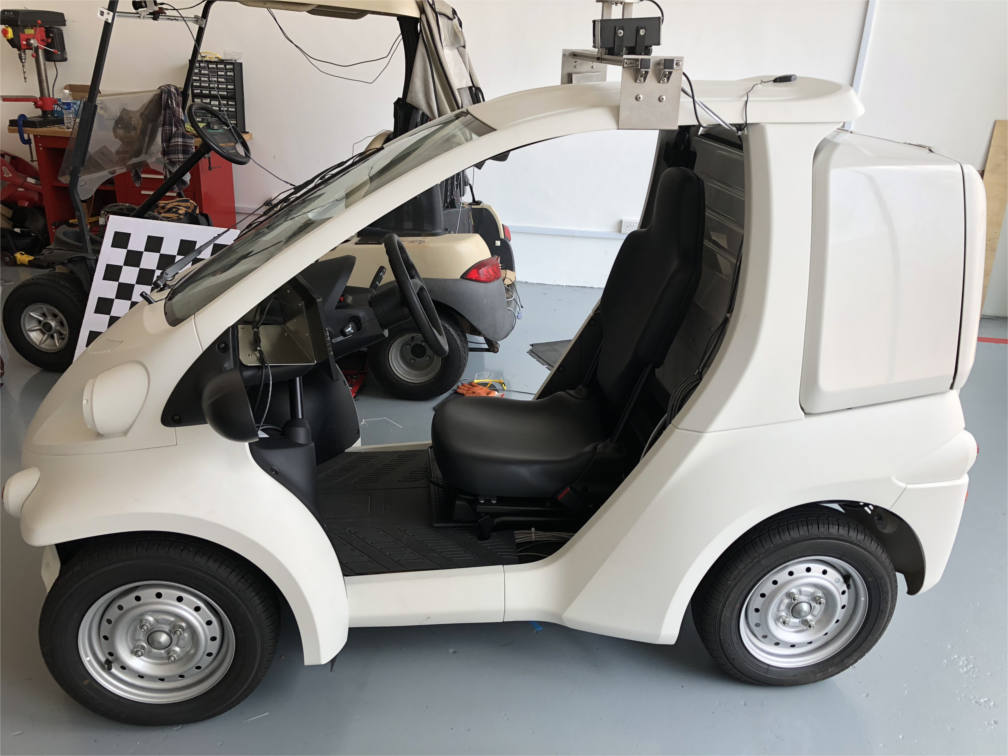
\includegraphics[width=0.8\textwidth]{singpilot.jpg}
  \end{figure}

\end{frame}

\begin{frame}{Localization of Autonomous Vehicles via Secure Sensor Fusion}
  \begin{columns}
    \begin{column}{0.48\textwidth}
      \begin{figure}
	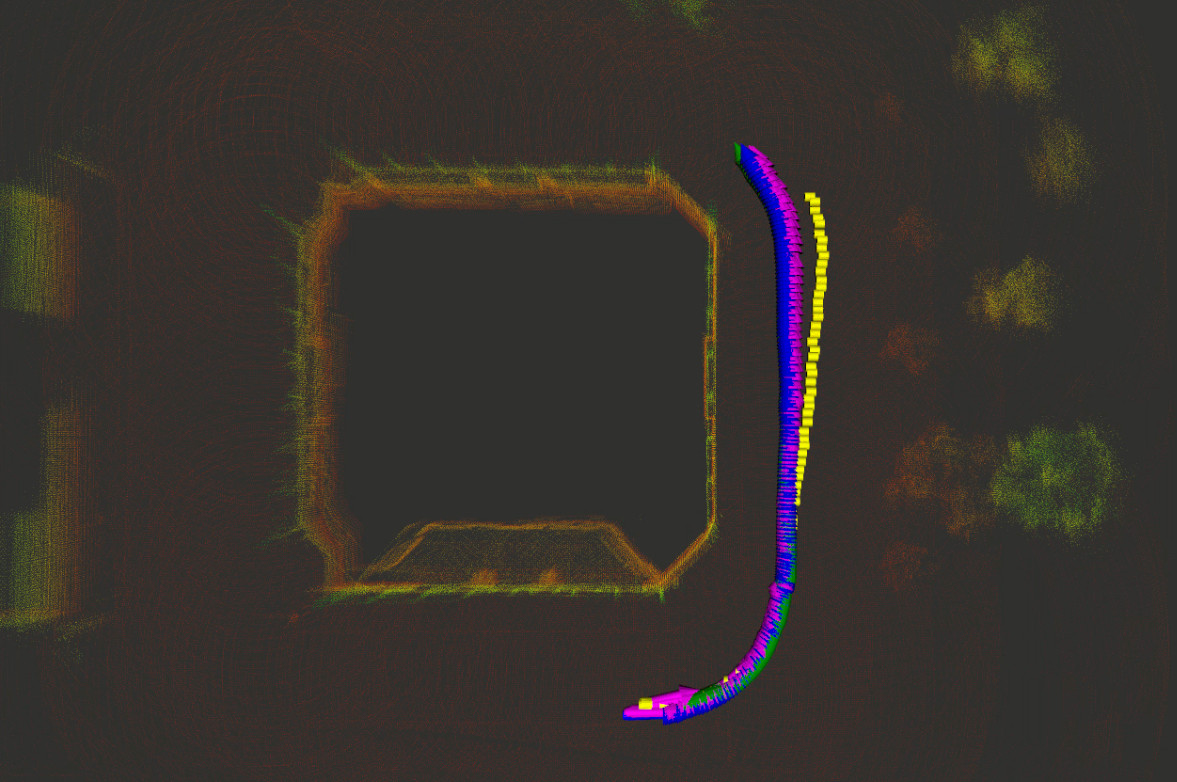
\includegraphics[width=\textwidth]{gnssdrift.jpg}
	\caption{EKF}
      \end{figure}
    \end{column}
    \begin{column}{0.48\textwidth} 		
      \begin{figure}
	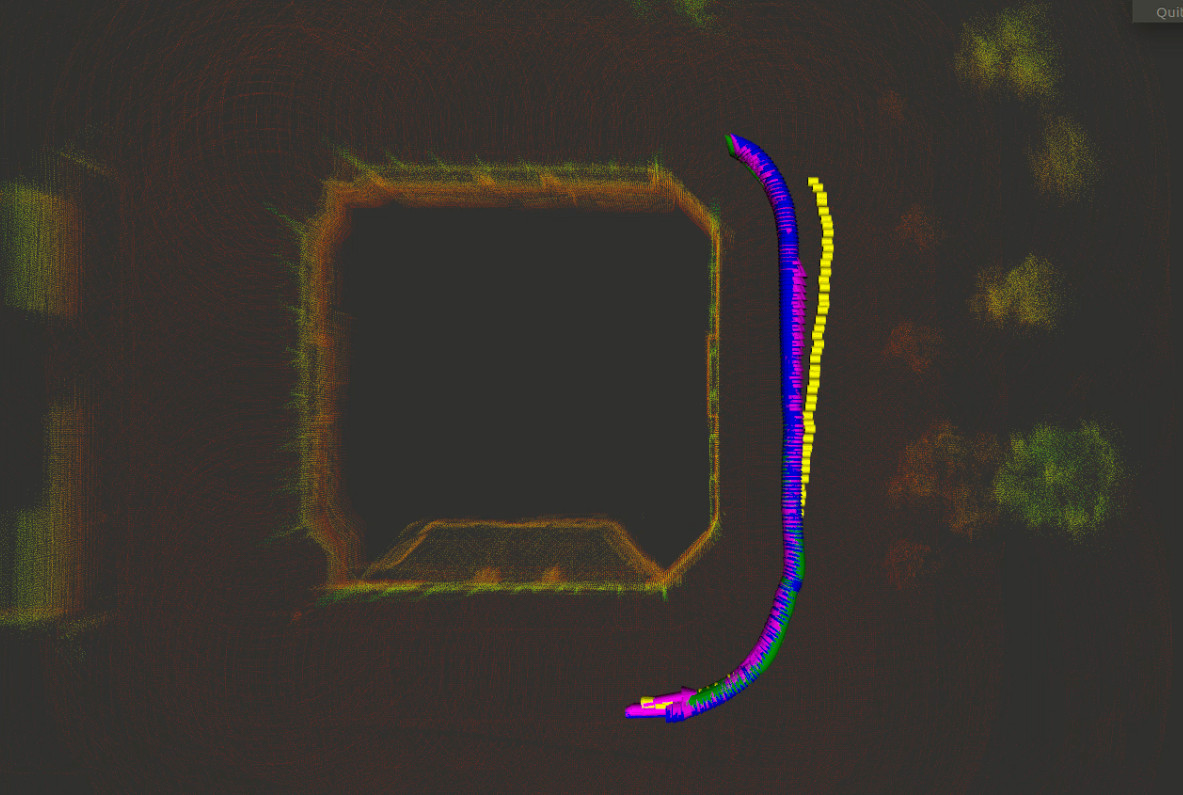
\includegraphics[width=\textwidth]{gnssdriftsafe.jpg}
	\caption{Secure EKF}
      \end{figure}
    \end{column}
  \end{columns}
\end{frame}


\section{Conclusion}

%\begin{frame}{Towards a Science of CPS Security}
%  \begin{itemize}
%    \item We consider both the static and dynamic state estimation problem in adversarial environment 
%    \item For static estimation, we propose a convex optimization based estimator and derive necessary and sufficient condition for its stability
%    \item For dynamic estimation, we propose a local filter + global fusion design:
%      \begin{enumerate}
%	\item In the absence of the attack, we recover the optimal Kalman filter with certain probabiliy
%	\item In the presence of the attack, we provide a sufficient condition for stability
%	\item For $A$ matrix whose unstable eigenvalues have geometric multiplicity of 1, the filter also achieves optimal security 
%      \end{enumerate}
%    \item Future directions: How to combine information security with system theory to provide defense in depth?
%  \end{itemize}
%\end{frame}
%
%\begin{frame}{Acknowledgement}
%  \begin{itemize}
%    \item Duo Han, Xinghua Liu, Zishuo Li
%    \item Lihua Xie, Emanuele Garone 
%    \item NTU Autonomous Driving Group: Danwei Wang, Jakub Tomasek, Qipeng Liu, Ehsan Mihankhah, Xiaoqiang Ren, Xiaoyu Mo 
%  \end{itemize}
%\end{frame}


\begin{frame}{Towards a Science of CPS Security}
  \begin{itemize}
  \item We consider intrusion detection problem in adversarial environment and propose an active detection scheme.
    \item We consider both the static and dynamic state estimation problem in adversarial environment 
    \item For static estimation, we propose a convex optimization based estimator and derive necessary and sufficient condition for its stability
  \item How to systematically design secure algorithms?
  \item How to combine information security with system theory to provide defense in depth?
  \end{itemize}
\end{frame}

\begin{frame}{Acknowledgement}
  \begin{itemize}
  \item Rohan Chabukswar, Sean Weerakkody, Hanxiao Liu, Jiaqi Yan, Zishuo Li
  \item Bruno Sinopoli, Lihua Xie, Karl H. Johansson
  \end{itemize}
\end{frame}

%\begin{frame}[allowframebreaks]
%     \printbibliography
%\end{frame} 

\begin{frame}[standout]
  感谢聆听!请各位老师批评指正
\end{frame}

\end{document}
